%---------------------------------------------------------------------------%
%-                                                                         -%
%-                           LaTeX Template                                -%
%-                                                                         -%
%---------------------------------------------------------------------------%
%- Copyright (C) Huangrui Mo <huangrui.mo@gmail.com>
%- This is free software: you can redistribute it and/or modify it
%- under the terms of the GNU General Public License as published by
%- the Free Software Foundation, either version 3 of the License, or
%- (at your option) any later version.
%---------------------------------------------------------------------------%
%->> Document class declaration
%---------------------------------------------------------------------------%

\documentclass[doublesided]{Style/ucasthesis}%
%- Multiple optional arguments:
%- [<singlesided|doublesided|printcopy>]% set one or two sided eprint or print
%- [draftversion]% show draft version information
%- [fontset=<fandol|...>]% specify font set to replace automatic detection
%- [scheme=plain]% thesis writing of international students
%- [standard options for ctex book class: draft|paper size|font size|...]%
%---------------------------------------------------------------------------%
%->> Document settings
%---------------------------------------------------------------------------%
\usepackage[super,myhdr,list]{Style/artratex}% document settings
%- usage: \usepackage[option1,option2,...,optionN]{artratex}
%- Multiple optional arguments:
%- [bibtex|biber]% set bibliography processor and package
%- [<numbers|super|authoryear|alpha>]% set citation and reference style
%- <numbers>: textual: Jones [1]; parenthetical: [1]
%- <super>: textual: Jones superscript [1]; parenthetical: superscript [1]
%- <authoryear>: textual: Jones (1995); parenthetical: (Jones, 1995)
%- <alpha>: textual: not available; parenthetical: [Jon95]
%- [geometry]% reconfigure page layout via geometry package
%- [lscape]% provide landscape layout environment
%- [myhdr]% enable header and footer via fancyhdr package
%- [color]% provide color support via xcolor package
%- [background]% enable page background
%- [tikz]% provide complex diagrams via tikz package
%- [table]% provide complex tables via ctable package
%- [list]% provide enhanced list environments for algorithm and coding
%- [math]% enable some extra math packages
\usepackage{Style/artracom}% user defined commands
%---------------------------------------------------------------------------%
%->> Document inclusion
%---------------------------------------------------------------------------%
%\includeonly{Tex/Chap_1,...,Tex/Chap_N}% selected files compilation
%---------------------------------------------------------------------------%
%->> Document content
%---------------------------------------------------------------------------%
\newcommand*{\noaddvspace}{\renewcommand*{\addvspace}[1]{}}
\addtocontents{lof}{\protect\noaddvspace}
\addtocontents{lot}{\protect\noaddvspace}

\begin{document}
%-
%-> Frontmatter: title page, abstract, content list, symbol list, preface
%-
\frontmatter% initialize the environment
%---------------------------------------------------------------------------%
%->> 封面信息及生成
%---------------------------------------------------------------------------%
%-
%-> 中文封面信息
%-
\confidential{}% 密级:只有涉密论文才填写
\schoollogo{scale=0.5}{nwu_logo}% 校徽
\title{低分辨率环境下的微表情识别}% 论文中文题目
\author{李桂锋}% 论文作者
\advisor{\hspace{+3.0em}彭进业~教授~西北大学}% 指导教师:姓名 专业技术职务 工作单位
%\advisorsec{}% 指导老师附加信息 或 第二指导老师信息
\degree{硕士}% 学位:学士、硕士、博士
\degreetype{工学}% 学位类别:理学、工学、工程、医学等
\major{电子与通信工程}% 二级学科专业名称
\institute{信息科学与技术学院}% 院系名称
\chinesedate{2019~年~6~月}% 毕业日期:夏季为6月、冬季为12月
%-
%-> 英文封面信息
%-
\englishtitle{Micro-expression Recognition\\Under Low-resolution Case}% 论文英文题目
\englishauthor{Li Guifeng}% 论文作者
\englishadvisor{Supervisor: Peng Jinye Professor}% 指导教师
\englishdegree{Master}% 学位:Bachelor, Master, Doctor。封面格式将根据英文学位名称自动切换,请确保拼写准确无误
\englishdegreetype{Engineering}% 学位类别:Philosophy, Natural Science, Engineering, Economics, Agriculture 等
\englishthesistype{thesis}% 论文类型: thesis, dissertation
\englishmajor{Electronics and Communication Engineering}% 二级学科专业名称
\englishinstitute{ }% 院系名称
\englishdate{June 2019}% 毕业日期:夏季为June、冬季为December
%-
%-> 生成封面
%-
\maketitle% 生成中文封面
\makeenglishtitle% 生成英文封面
%-
%-> 作者声明
%-
\makedeclaration% 生成声明页
%-
%-> 中文摘要
%-
\chapter{摘\quad 要}\chaptermark{摘\quad 要}% 摘要标题
\setcounter{page}{1}% 开始页码
\pagenumbering{Roman}% 页码符号

人脸表情在我们的社交互动中发挥着重要作用,因为它传达了丰富的信息。我们可以从一张人脸图像中阅读很多内容,但是如果没有特殊设备,我们也无法感知到这些信息。本文采用计算机视觉方法分析肉眼难以察觉的两种微妙的面部信息:微表情和心率。
微表情是快速、不自主的面部表情,揭示了人们不打算表达的情感。人们很难感知微表情,因为它们太快和微妙,因此自动微表情分析是很有价值的工作,具有重大的应用前景。本文综述了微表情研究的进展,并分四部分工作进行描述。 1)我们介绍了第一个自发的微表情数据库—SMIC。缺乏数据阻碍了微表情的分析研究,因为很难收集自发的微表情。引入用于诱导和注释SMIC的协议以帮助未来的微表情收集。 2)引入了包括三个特征和视频放大过程的框架用于微表情识别,其优于两个微表情数据库上的其他最先进的方法。 3)描述了一种基于特征差异分析的微表情定位方法,该方法可以从自发的长视频中发现为微表情。 4)提出了一种自动微表情分析系统(MESR),用于发现并识别微表情。
心率是我们健康和情绪状态的重要指标。传统的心率测量需要皮肤接触,不能远程应用。我们提出了一种方法,可以对抗照明变化和头部运动,并从彩色面部视频远程测量心率。我们还应用该方法来解决面部反欺骗问题。我们展示了基于脉冲的特征比传统的基于纹理的特征更能够抵抗看不见的掩模欺骗。我们还表明,所提出的基于脉冲的特征可以与其他特征相结合,以构建用于检测多种类型的攻击的级联系统。
最后,我们总结了工作的贡献,并基于当前工作的局限性提出了关于微表情和心率研究的未来计划。还计划将微表情和心率(可能还有来自面部的其他微妙信号)结合起来构建用于情感状态分析的多模式系统。

微表达是一种基本的非言语行为,它能忠实地表达人类隐藏的情感。它在国家安全、计算机辅助诊断等领域有着广泛的应用,促使我们对自动微表情识别进行研究。但从监控视频中获取的图像容易出现质量问题,导致实际应用困难。由于捕获的图像质量较低,现有的算法无法达到预期的效果。为了解决这个问题,我们进行了全面的研究

\keywords{微表情识别,监控视频,低分辨率,超分辨率,Fast LBP-TOP}% 中文关键词
%-
%-> 英文摘要
%-

\chapter{ABSTRACT}\chaptermark{ABSTRACT}% 摘要标题

\noindent
The face plays an important role in our social interactions as it conveys rich sources of information. We can read a lot from one face image, but there is also information we cannot perceive without special devices. The thesis concerns using computer vision methodologies to analyse two kinds of subtle facial information that can hardly be perceived by naked eyes: the micro-expression (ME), and the heart rate (HR\\
\\
MEs are rapid, involuntary facial expressions which reveal emotions people do not intend to show. It is difficult for people to perceive MEs as they are too fast and subtle, thus automatic ME analysis is valuable work which may lead to important applications. In the thesis, the progresses of ME studies are reviewed, and four parts of work are described. 1) We introduce the first spontaneous ME database, the SMIC. The lacking of data is hindering ME analysis research, as it is difficult to collect spontaneous MEs. The protocol for inducing and annotating SMIC is introduced to help future ME collections. 2) A framework including three features and a video magnification process is introduced for ME recognition, which outperforms other state-of-the-art methods on two ME databases. 3) An ME spotting method based on feature difference analysis is described, which can spot MEs from spontaneous long videos. 4) An automatic ME analysis system (MESR) was proposed for firstly spotting and then recognising MEs\\
\\
The HR is an important indicator of our health and emotional status. Traditional HR measurements require skin-contact which cannot be applied remotely. We propose a method which can counter for illumination changes and head motions and measure HR remotely from color facial videos. We also apply the method for solving the face anti-spoofing problem. We show that the pulse-based feature is more robust than traditional texture-based features against unseen mask spoofs. We also show that the proposed pulse-based feature can be combined with other features to build a cascade system for detecting multiple types of attacks.\\
\\
At last, we summarize the contributions of the work, and propose future plans about ME and HR studies based on limitations of the current work. It is also planned to combine the ME and HR (maybe also other subtle signals from face) to build a multimodal system for affective status analysis.\\
\\
Micro-expression is an essential non-verbal behavior that can faithfully express the human's hidden emotions. It has a wide range of applications in the national security and computer aided diagnosis, which encourages us to conduct the research of automatic micro-expression recognition. However, the images captured from surveillance video easily suffer from the low-quality problem, which causes the difficulty in real applications. Due to the low quality of captured images, the existing algorithms are not able to perform as well as expected. For addressing this problem, we conduct a comprehensive study about the micro-expression recognition problem under low-resolution cases with face hallucination method. The experimental results show that the proposed framework obtains promising results on micro-expression recognition under low-resolution cases.

\englishkeywords{Micro-expression recognition, Surveillance video, Low-resolution, Super-resolution, Fast LBP-TOP}% 英文关键词
%---------------------------------------------------------------------------%
% title page, abstract, dedication
% \chapter{插图索引}
\chaptermark{插图索引}

\listoffigures
% list of symbols
% \chapter{表格索引}
\chaptermark{表格索引}

\listoftables
% list of abbr
{% content list region
\noindent
\linespread{1.2}% local line space
%\intotoc{\contentsname}% add link to contents table and bookmark
\let\oldnumberline\numberline%
\renewcommand{\numberline}{\figurename~\oldnumberline}%
\intotoc{\listfigurename}% add link to contents table and bookmark
\listoffigures% figures catalog
\renewcommand{\numberline}{\tablename~\oldnumberline}%
\intotoc{\listtablename}% add link to contents table and bookmark
\listoftables% tables catalog
\chapter{符号对照表}
\chaptermark{符号对照表}

\nomenclatureitem{符号}{\hfill \makebox[0.4\textwidth]{符号名称}}
\nomenclatureitem{$\bigotimes$}{\hfill \makebox[0.4\textwidth]{哈达玛积}}
\nomenclatureitem{$\boldsymbol{\lambda}$}{\hfill \makebox[0.4\textwidth]{惩罚系数}}
\nomenclatureitem{$\boldsymbol{\phi (\cdot )}$}{\hfill \makebox[0.4\textwidth]{从原始空间到无限维再生核希尔伯特空间的映射}}
\nomenclatureitem{$\boldsymbol{\omega}$}{\hfill \makebox[0.4\textwidth]{结合系数}}
\nomenclatureitem{$\boldsymbol{\eta }$}{\hfill \makebox[0.4\textwidth]{基于像素的正则项系数}}
\nomenclatureitem{$\boldsymbol{\alpha}$}{\hfill \makebox[0.4\textwidth]{基于块的正则项系数}}
\nomenclatureitem{$\boldsymbol{\sigma}$}{\hfill \makebox[0.4\textwidth]{均方误差系数}}
% list of symbols
\chapter{缩略语对照表}
\chaptermark{缩略语对照表}

\nomenclatureitem[\textbf{中文对照}]{\textbf{缩略语}}{\textbf{英文全称}}
\nomenclatureitem[微表情]{ME}{Micro Expression}
\nomenclatureitem[时间插值模型]{TIM}{Time In Model}
\nomenclatureitem[微表情识别标准测验]{BART}{Brief Affect Recognition Test}
\nomenclatureitem[面部动作编码系统]{FACS}{Facial Action Coding System}
\nomenclatureitem[动作单元]{AU}{Action Unit}
\nomenclatureitem[微表情训练工具]{METT}{Micro Expression Training Tool}
\nomenclatureitem[特征差异]{FD}{Feature Difference}
\nomenclatureitem[峰值检测]{PD}{Peak Detection}
\nomenclatureitem[留一法]{LOSO}{Leave One Subject Out}
% list of abbr
}
{% content list region
\noindent
\linespread{1.2}% local line space
\tableofcontents% contents catalog
}

%\intotoc{\contentsname}% add link to contents table and bookmark
%-
%-> Mainmatter
%-
\mainmatter% initialize the environment
%---------------------------------------------------------------------------%
%->> Main content
%---------------------------------------------------------------------------%
\chapter{绪论}\label{chap:introduction}

微表情(Micro Expressions),心理学名词,心理应激微反应的一部分,是人类表达自身情感信息的重要非语言性行为。微表情从人类本能出发,在大多数情况下,不受思想的控制,无法掩饰,也不能伪装\citep{Haggard1966}。因为它无法伪装的特性起初被人们用来作为鉴谎的辅助工具,随着人们对其不断深入的研究发现它在临床诊断、司法系统等有着很高的应用价值。近几年来随着计算机技术的不断发展,人们利用计算机视觉对微表情识别研究有了突飞猛进的成果,但就目前而言,还没有团队在低分辨率环境下对微表情做任何研究。本文从实际应用的角度出发,分析实际场景中面临的各种低质量问题,分别使用传统机器学习方法和深度学习方法对微表情识别。

本章主要阐述微表情识别研究的意义和低分辨率环境下微表情识别的重要性,国内外对微表情识别相关的研究和发展趋势,最后概述了文章的内容和结构分配。

\section{研究背景与意义}

达尔文在1872年出版了《The Expression of Emotions in Man and Animals》,从此拉开了人类对面部表情的系统性研究。时至今日,人类对面部表情的研究已经非常丰富与成熟,但主要关注的是显而易见的宏观表情(Macro Expressions),虽然在1966年Haggard和Isaacs首次提出了微表情现象(Micro-momentary Facial Expressions),但当时并未引起人们的普遍重视。直到三年后(1969年),Ekman和Friesen在临床发现了微表情,这一发现奠定了微表情在临床辅助治疗上的重要地位\citep{ekman1969nonverbal},也开启了微表情的研究热潮。

本节将从微表情研究的意义和计算机视觉对微表情研究的意义两方面分析。

\subsection{微表情研究的意义}

加利福尼亚大学洛杉矶分校的心理学教授Albert Mehrabian在上世纪六十年代发现了人际交流中的“55384”原则,他提出有效的沟通技巧应该包含三大要素:身体语言、声音和谈话内容\citep{Mehrabian1967Inference}。其中谈话内容传递的信息量是总信息量的7\%,声音(包括交谈时的语气、音调和音量)传递的信息量占总信息量的38\%,剩下的55\%来自身体语言(包括谈话期间身体姿势、肢体动作、面部表情、眼神和目光等),也就是说身体语言比谈话内容能传达更多有价值的信息。论文中阐明,出现这种情况的主要原因是谈话内容(口头语言)可以有意识地被控制,而身体语言这种非语言行为是无意识的举动,人类的主观意识很难控制动作语言行为。身体语言由三部分构成:表情语言、动作语言和空间语言。表情语言指的是通过面部肌肉运动和眼睛神态所传递出来的思想感情,动作语言指人类通过身体各个部位的动作或姿态来传递感情,空间语言主要指由个体与个体之间所保持的间距所形成的一种信息表达方式。在这三种身体语言中最容易被观察到的就是表情语言,艾伯特教授的这项发现说明了表情语言的重要性。

神经学家Paul Donald MacLean于上世纪五十年代提出了“大脑三位一体”理论(The Triune Brain),他认为人类颅腔内的脑并非只有一个,而是三个,这三个脑作为人类不同进化阶段的产物,按照出现顺序依次覆盖在已有的脑层之上,如同考古遗址一样\citep{Brain1999Kazlev}。根据在进化史上出现的先后顺序,他将人脑分成“爬行动物脑”(Reptilian brain)、“古哺乳动物脑”(Paleomammalian Brain)和“新哺乳动物脑”(Neomammalian Brain)三大部分,它们分别对应人脑的脑干(Archipallium)、边缘系统(Limbic System)和新皮质(Neocortex),它们共同控制着人类的身体行为。新皮质被称作“爱说谎的大脑”,经常会因为当事人的某种需要而出现说谎的现象。语言等由新皮质大脑控制的行为是不可信的,欺骗的嫌疑很大,想要得知对方内心的真实感受,必须观察对方边缘系统所控制的表情或肢体动作。边缘系统是控制人类情感的中心,管理着人类的非语言行为表达,因此是分析身体语言的重点。让人不加思索的产生本能反应是它的一大特点,它反映出了一个人最真实的一面,这很难被控制和掩饰。比如,当听到刺耳的噪音时你会不自主地捂住耳朵、手碰到高温或极寒物体时会马上缩回等。所以边缘系统的行为是诚实可信的行为,是人类的思想、感觉和意图的真实反应,也是人类生存、本能的反应,它属于微反应中除微语言以外的非语言行为反应,它包括了微动作(Micro Action)、微表情。

从上述例子可以看出,有关微表情的研究在心理学和神经学两大学科都有着充分的理论依据。Ekman等人在临床上发现微表情是来自于观看一位有自杀倾向的精神病患者的视频,视频中患者在回答医生问题时表现的很开心,没有任何想要自杀的异常迹象,但在随后的二次会谈中患者向医生承认其状况并未好转,而且她曾隐藏了自杀的计划。Ekman和 Friesen在逐帧慢放视频时发现确实存在两帧和绝望有关的负面表情,这与患者的二次会谈内容相吻合,但只持续了1/12 s。之后的几十年里Ekman和他的同事继续研究微表情,在不断的实践中量化并定义了微表情,这也引起了越来越多学术界和商业界人士的兴趣,目前微表情已经被应用到了众多领域,比如国家安全、司法系统、政治选举、临床诊断、公共管理和教育领域等\citep{Chiu2014The}。

\subsection{计算机视觉对微表情研究的意义}

我们人类是优秀的“人脸识别专家”,我们已经习惯甚至并没有意识到这一点。与其他类型的物种相比,我们人类为应对复杂的社交交互问题,大脑已经开发了特殊的识别脸部信息的功能模块,以便我们更好地从人脸中获取更丰富的信息,所谓“察言观色”就是很好的佐证。当然,人脸也是丰富的视觉信息的来源之处,我们可以从人脸中读取很多信息。比如眼前之人如果是著名人士,我们可以立即认出他或她,如果是陌生人,我们可以对这个人的性别、年龄、种族等做出基本正确的猜测,同时如果该人脸存在表情,我们也可以大致感知他或她的情绪状态。然而尽管我们是人脸识别专家,但这并不意味着我们已经解析出了全部的人脸信息,因为仍然存在部分无法用肉眼读取的深层次信息。

与其他感官(例如听觉和嗅觉)相比,我们的视觉认知功能在我们的大脑中更加精巧地被构建。然而,我们获取视觉信息的能力仍然受到生理机制的限制。超出我们感知范围的视觉变化(在空间域中太微妙或在时域中太快)将被我们的眼睛忽略。比如我们很难从人脸上观察到某个微表情,因为微表情会短暂且快速地发生,所涉及的肌肉运动强度也非常微弱,甚至表情发出者和观察者都察觉不到,尤其在高风险条件下微表情出现的机率更高,被察觉的可能性也更低。研究人员经过严密的统计,发现微表情持续时间最长为1/2秒而最短只有1/25秒,所涉及的肌肉运动强度更是微乎其微,而正常的表情(宏观表情)一般持续时间在1/2秒到5秒之间,有一个起承转合的过程。\citep{Yan2013How, matsumoto2011evidence, Porter2008Reading}。

由于微表情识别务实的使用价值,其提出者Ekman从2005年开始对英国情报机构、美国中央情报局等各国机构进行微表情识别培训,而那时他已经71岁高龄了\citep{Lie2010to}。他教辩护律师、健康专家、扑克选手,甚至对配偶心怀猜疑的人识破谎言,并且制作了网络课程。但他坦言人类对于微表情的识别能力终归是有限的,不仅要花费大量的人力和物力培训微表情识别专家,而且准确度不高,同时还伴有影响正常生活的风险\citep{Ekman2010A}。Ekman曾说自己的识谎能力影响到了日常生活,他从不试图去识破周围朋友、亲戚的微表情,“去揭露每个人的微表情,揭穿每个人的谎言,这只会让自己的生活痛苦万分”。

同时当前对微表情研究的研究中,需要使用FACS(Facial Action Coding System)对包含被试微表情的视频进行逐帧的编码\citep{ekman1978facial}。但是,不仅FACS编码的训练比较费时,编码者一般都需要接受100小时的训练才能达到初步熟练的程度;而且使用FACS进行编码也很费时,编码1分钟的视频平均需要2个小时\citep{Maja2009Machine}。为了更快地对基本表情编码,在FACS基础上,研究者发展出了一套附加的编码系统EMFACS(Emotion Facial Action Coding System),但人工对视频进行逐帧编码依然费时费力,这极大地限制了目前的微表情研究。因此,有效的微表情自动分析工具是开展微表情表达研究需要解决的一个重要问题。

计算机的发明是为了帮助人类更好地处理人类不想去处理的任务,而识别人脸微表情这种会影响到日常生活的任务就是计算机存在的价值所在。而且当通过摄像机和计算机系统对待分析者分析时,不仅采集到的表情真实可靠(采集中采集对象并不知情,不存在任何干扰)而且通过计算机算法可以发现细微的人类无法察觉的表情变化,并且已经有大量的实验证明计算机的识别能力确实高于人类\citep{Li2017Towards}。我们可以更好更快的训练计算机完成人类能够完成的任务,如人脸检测、人脸识别,同时我们还可以训练计算机执行我们无法完成的任务,如捕获肉眼难以察觉的细微信息\citep{Doctoral2017Li}。

\section{国内外研究现状}\label{sec:system}

\subsection{人工微表情识别训练工具研究}

早期研究中,研究人员注重于测量或训练个体的微表情识别能力。Ekman 和Friesen在1974年制定了第一个微表情识别标准测验机制——BART(Brief Affect Recognition Test),但当时的微表情识别标准测验有着很大的缺陷,它所呈现的微表情是孤立的呈现,这与现实生活中微表情的动态呈现方式完全不相符,这样的测验没有任何生态效度\citep{Ekman1974Detecting, 殷明2016微表情}。1978年,Ekman发布了面部动作编码系统FACS,他们将人脸部的肌肉划分为43块,将它们随机组合获得了1万多种表情,但其中只有3000种具有情感意义,Ekman等人又根据人脸解剖学特点,将这43块肌肉划分成相互独立又相互联系的运动单元(Action Unit,AU),分析这些运动单元的运动特征和其所控制的主要区域,将这些信息与相关的表情匹配就能得出面部表情的标准运动。为了克服BART的缺陷, Matsumoto等人在2000年开发了更完善的微表情识别测量工具(Japanese and Caucasian Brief Affect Recognition Test,JACBART),该测验具有很好的可信度和严密的实验过程\citep{Matsumoto2000A}。Ekman等人在2002年根据日本人与高加索人短暂表情识别测验开发出了一个新的微表情识别训练工具METT(Micro Expression Training Tool),该训练工具有7种基本情绪的微表情,包括悲伤、恐惧、愤怒、厌恶、轻蔑、惊讶和高兴,METT 被应用在多种人群和领域,且对微表情受训者的识别能力有明显的提升\citep{ekman2003mett}。

\subsection{自动微表情识别研究}

除上述通过训练提升人工识别能力外自动地微表情识别系统也在如火如荼的发展中,研究者们已经开发出很多相关的算法,甚至在某些数据集的准确度可达90\%以上,但这些数据集有个明显的缺点,所有的微表情均为摆拍(Posed),这一缺点有其产生的必然性,但也严重违背了微表情的定义。为了解决这一问题,国内外的研究团队相继发表了自发微表情数据集,如中科院心理所分别在2013年和2014年发布了CASME\citep{Yan2013CASME}和CAMSE II\citep{Yan2014CASME}两个版本的数据集,后者比前者有着更高的时空分辨率和更多的数据量,但参与者全部为蒙古利亚人种(中国人),在数据的多样性上有一定的不足;芬兰奥卢大学的CMVS团队在2013年发布了SMIC数据集\citep{Li2013A},包括8名高加索人种和8名蒙古利亚人种,同时数据集中包含了高速视频数据(High speed video,HS)、近红外视频数据(Near infrared videos,NIR)和普通彩色视频数据(Normal color video,VIS);英国曼彻斯特城市大学在2017年发布了SAMM数据集\citep{Davison2018SAMM},是目前发表最新的数据集,包括了几乎全部的人种(蒙古利亚人种、高加索人种、尼格罗人种和大洋洲人种)和均衡的性别比,但其数据集只包含了高速灰度视频数据(见表~\ref{tab1})。优秀的数据集提供了良好的实验基础,自动微表情识别系统的研究主要集中在微表情检测(Micro-expression Spotting)和微表情识别(Micro-expression Recognition)。

微表情的检测指在一个图像序列(视频帧)中检测微表情发生的起始时间点。有许多研究致力于类似的任务,如检测普通的人脸表情、眨眼和人脸AU\citep{zeng2006spontaneous,Kr2012Eye, Liwicki2012Incremental},以及各种有效的算法被提出,与微表情识别研究相比,微表情检测的研究较少。由于缺乏自发的微表达数据,大多数早期的微表达检测研究多采用摆拍的微表情数据。Shreve等首次先提出了一种基于应变的光流方法来识别视频中的宏表情(普通人脸表情,微表情的反义词)和微表情,在USF-HD数据集(摆拍的数据集)中进行了测试,同时他们还对从在线视频中收集的28个微表情进行了测试,但是这个数据集很小,没有发表\citep{shreve2009towards, Shreve2011Macro}。在另一组研究中,Polikovsky等人提出了一种新的微表情检测方法,他们使用三维梯度直方图作为特征描述符,对中性面部微表情帧进行不同阶段(起始、顶峰和终止)分类\citep{Polikovsky2009Facial, Polikovsky2013Facial}。在他们的研究中,将微表情检测任务作为分类任务,并训练模型根据所涉及动作的阶段将视频片段分为四类。关于Polikovsky的研究,有一点很好,那就是作者试图在一个精细的层面上构建微表情的时间范围。这可能适用于摆拍的微表情片段,因为它们具有相似的时间结构,但不适用于自发的微表情,因为在真实场景中,微表情在其时间范围上存在显著差异。分类任务需要对视频预分割,这在实际应用中也是一个问题。Wu等人提出利用Gabor滤波器构建微表情识别系统进行微表情检测\citep{Qi2011The}。该方法在METT训练数据上进行了测试,取得了良好的效果。但有一点需要说明的是,METT训练样本完全是合成的视频片段(在一系列相同的中性人脸图像中间插入一张有情感的人脸图像)。在这些视频片段中,表情的“开始”和“结束”非常的尖锐和突然,上下文界线也非常清晰,所以它们根本不能代表计算机真正的微表情检测问题。

虽然上述研究可能会为微表情检测提供潜在的贡献,但一个主要的缺点是,它们仅在摆拍的(或METT等合成的)微表达数据集上进行了测试。与自发微表情相比,提出的数据更容易完成微表情的检测任务。摆拍或合成的微表情数据通常具有相似的时间范围结构,即人为控制的起止时间点,这与自发微表情之间存在显著差异。考虑到视频的上下文,摆拍的微表情片段通常在视频中会禁止无关的动作,所以摆拍的微表情片段通常具有更清晰的上下文。自发微表情视频的情况更加复杂,由于普通人脸表情(包含相同或相反的情绪价\citep{Warren2009Detecting})、眨眼和其他头部动作也可能发生,并且还可能与自然情绪相互重叠。这些在自发微表达数据中遇到的挑战,在以往的研究中利用摆拍的微表情数据都无法解决,因此利用自发微表情数据进行微表情检测还需要更多的工作。
论文\citepns{pfister2011recognising}和其他几项研究使用了一种更简单的方法,即微表达“探测”来解决这个问题\citep{ruiz2013encoding, Davison2014Micro, Yao2014Micro}。在这些研究中,微表情检测被视为二分类问题,一组带标签的微表达片段与另一组非微表达片段进行分类。这些研究都是在自发微表情数据集中测试的,这是一个很大的优点。但是对于分类任务,训练和测试视频都需要进行适当的分割,这在实际应用中可能会遇到困难。二分类方法与直接从长视频中提取自发微表情的实际应用目标仍有较大差异。Li等人提出了一种将特征差异(Feature Difference,FD)比较和峰值检测(Peak Detection,PD)相结合的微表情识别框架,这种方法是第一个用于真实微表情数据集检测微表情且行之有效的方法\citep{pfister2011recognising}。在最近的另一篇文章中作者提出了一种基于概率框架的随机游走模型(Random walk model)来检测微表情,通过几何变形建模从视频片段中识别自发微表情片段,该方法被证明对SMIC和CASMEII都是有效的\citep{Xia2016Spontaneous}。

微表情识别的任务类似于普通人脸表情识别,差异处在于微表情片段(包含微弱面部运动的起始到终止的帧序列)的标签,具体是指根据表达的情感内容训练一个分类器将其分类为两个或两个以上的类别(例如快乐、悲伤等)。在众多已发表的文献中微表情识别的研究比微表情检测的研究更为突出,在摆拍和自发的数据集上提出并测试了很多算法。早期的工作都是从摆拍的微表情数据开始的。Polikovsky和Kameda等人采用三维梯度描述符对AU标记的微表情进行识别,将提出的方法在自己采集的摆拍微表情数据上进行了测试\citep{Polikovsky2013Facial}。Wu等人将Gentleboost和支持向量机(Support Vector Machine,SVM)分类器结合,在METT训练工具中识别合成的微表达样本。随着自发微表达数据库的出现,利用自发微表达数据库进行微表达识别的研究也越来越多。2011年,论文\citepns{pfister2011recognising}提出了第一个微表情识别方法,并在第一版的SMIC数据集上取得了很好的效果(第一版的SMIC数据集包含77个自发的微表情样本)。该方法采用时间插值模型(temporal interpolation model,TIM)对微表情计算帧数,将其与和多核学习(Multiple Kernel Learning,MKL)结合捕获图像序列的主要变化,使用三正交平面的局部二值模型(Local Binary Patterns on Three Orthogonal Planes,LBP-TOP)特征作为描述符提取动态纹理作为微表情识别的特征,再用随机森林(Random forest,RF)作为分类器分类。这是首次尝试构建一个可行的方法来识别这些细微的面部行为,并在77个微表情样本上取得了很好的效果(二分类准确度为71.4\%)。同样的方法在新版本的SMIC数据集上进行了测试,在包含164个微表情的SMIC-HS数据集上得到了48.78\%(三分类)的识别结果。此后,论文\citepns{pfister2011recognising}的研究结果被许多其他研究人员引用为微表情识别研究的基准。Ruiz-Hernandez和Pietikäinen等人利用二阶高斯流的再参数化来生成更鲁棒的直方图,在第一版SMIC数据库上得到了比论文\citepns{pfister2011recognising}更好的识别结果\citep{ruiz2013encoding}。Huang等人通过在时空域中的积分投影获得被试者(目标)的形状属性,将形状属性与时空域上的纹理信息结合组成新的特征,提出了时空局部量化模式(SpatioTemporal Completed Local Quantization Patterns,STCLQP)作为微表情识别的特征,在SMIC上实现了64.02\%的精度\citep{Huang2015Facial}。

几个其他的微表情识别研究使用了CASMEII微表情数据库。Wang等人从张量独立颜色空间(非普通的RGB颜色空间,Tensor independent color space,TICS)中提取LBP-TOP进行微表情识别,并在CASMEII数据集进行测试\citep{wang2014micro2}。Wang等人在其另一篇论文中,将局部时空方向特征与鲁棒主成分分析(Principal Component Analysis,PCA)的稀疏部分相结合一起用于微表情识别,在CASMEII上实现了65.4\%的准确率\citep{wang2014micro}。Wang等人提出利用6个交叉点的局部二值模式(LBP-Six Intersection Points,LBP-SIP)进行微表情识别,并在CASMEII和SMIC上进行了测试,该方法是减少了LBP-TOP中的冗余信息\citep{wang2014lbp}。Huang等人为了提高微表情的辨别力,提出一种新的基于Laplacian的特征选择方法,在已发表的数据集中得到了很好的识别效果\citep{xiaohua2017discriminative}。Wang等人提出了一种紧实的LBP-TOP描述符(Super-compact LBP-Three Mean Orthogonal Planes,MOP),MOP所描述的紧实鲁棒形式不仅保留了基本模式而且减少了影响编码特征判别的冗余\citep{wang2015efficient}。Hong等人为提高LBP-TOP在时空信息上的计算效率,引入了张量的概念,这加速从三维空间到二维空间的实现过程\citep{FLBPTOP_2016}。

除LBP及其变体外,部分研究人员致力于对光流特性的研究。如Liu等人提出利用主方向平均光流特征(Main direction Mean opticflow,MDMO)进行微表情识别,同时还考虑了局部统计运动和空间位置信息,在SMIC和CASMEII数据库上都取得了良好的性能,但是他们只使用了SMIC的第一个版本,而不是SMIC的完整版\citep{liu2016mainl}。Liong等人从光学应变量值得到一个时间段内人脸的细微相对位移量,并对局部特征赋予不同的权重,形成新的特征\citep{liong2014subtle}。Xu等人利用光流估计对微表情图像序列选择的粒度进行像素级对齐,得到主光流方向,将其作为精细的面部动态特征描述符\citep{xu2017microexpression}。

近年来,对微表情识别的研究十分活跃。到目前为止,大多数提出的方法都考虑使用基于纹理的特性来完成任务。时空纹理特征是描述面部运动的合适选择,但单独使用它们可能不足以进行微表情识别,识别性能仍有很大的提升空间。Li等人将低强度的微表情视频经过欧拉视频放大,在三个正交平面上利用不同的特征提取符提取特征对微表情进行识别。随后Li等人基于LBP-TOP的思想在三个正交平面上扩展了梯度方向直方图(HOG)和图像梯度方向直方图(HIGO)提出了HOG-TOP和HIGO-TOP。Song等人通过从面部和身体微弱运动中学习的稀疏编码来识别情绪,他们的微表情定义更加广泛,将身体部位(脸部除外)的姿势包括在内\citep{Song2013Learning}。Ngo等人提出了一种用于微表情图像序列预处理的选择性转移机(Selective Transfer Machine,STM),用于解决数据库中不平衡和不同面部形态的问题\citep{le2014spontaneous}。Lu等人发现微表情的图像序列在时空域中基于Delaunay三角归一化,提出了基于Delaunay的时间编码模型(Delaunay-based temporal coding model,DTCM)\citep{lu2014delaunay}。Oh等人通过Riesz小波变换获得多尺度单原信号,提取其幅值、相位、方向特征组成新的特征描述符进行微表情识别\citep{oh2015monogenic}。He等人提出了一种多任务的中层特征学习方法进行特征提取,该方法能够获得更具识别能力和泛化能力的中层特征\citep{he2017multi}。由于深度学习模型需要大量的数据进行训练,而现有的微表情数据还远远不够,但最近,Patel等人提出了一种利用深度学习模型解决微表情识别问题的方法\citep{Patel2016Selective}。作者建议选择性使用基于普通人脸表情数据库训练的卷积神经网络(Convolutional Neural Networks,CNN)模型的深度特征,但效果并不理想。Li等人发现微表情的峰值帧能够表达更丰富的情感,他们提出了一种在峰值帧应用深度神经网络的方法检识别表情,在CASME II上取得了不错的成果\citep{canYan18}。表~\ref{tab2}对目前提出的大多数方法做了列举。

\begin{table}[!htbp]
\centering
\caption{微表情的研究方法}
\label{tab2}
\footnotesize% fontsize
\setlength{\tabcolsep}{4pt}% column separation
\renewcommand{\arraystretch}{1.2}%row space
\begin{tabular}{c|c|c|c}
\hline
\multicolumn{2}{c|}{摆拍微表情数据集(Posed)} & \multicolumn{2}{c}{自发微表情数据集(Spontaneous)} \\ \hline
微表情检测 & 微表情识别 & 微表情检测 & 微表情识别 \\ \hline
\multirow{3}{*}{3D梯度} & \multirow{6}{*}{Gentleboost和SVM} & \multirow{6}{*}{特征差异与峰值检测} & TIM+MKL+LBP-TOP+RF \\
 &  &  & 二阶高斯射流的再参数化 \\
 &  &  & 从张量独立色彩空间中提取LBP-TOP \\
\multirow{4}{*}{Gabor滤波器} &  &  & 局部时空方向特征+鲁棒PCA \\
 &  &  & 低强度的微表情视频经过欧拉视频放大 \\
 &  &  & 基于普通表情的迁移学习 \\
 & \multirow{5}{*}{人脸与身体微弱运动结合} & \multirow{5}{*}{基于概率的随机游走模型} & LBP-SIP、STM、MOP、STCLQP、DTCM \\
\multirow{4}{*}{应变的光流方法} &  &  & Riesz小波变换、光流估计 \\
 &  &  & 引入张量概念的Fast LBP-TOP \\
 &  &  & MDMO+局部运动+空间位置 \\
 &  &  & HOG/HIGO-TOP \\ \hline
\end{tabular}
\end{table}

\section{本文的研究内容}

本文简单介绍了微表情识别的研究现状和基本方法,以及其不容小觑的应用价值。然而,目前的微表情研究都是基于高质量数据集的基础上展开的,例如SMIC数据集的人脸分辨率为$190\times230$像素,最新发布的SAMM数据集的人脸分辨率达到$400\times400$像素之高,但在实际应用中由于图像采集设备的机能限制,难免会遇到低像素的视频数据,这严重影响了几乎所有的微表情识别算法的性能,为了解决这一问题,本文提出了专门针对低分辨率环境下的微表情识别方法:按照常规方法对视频做预处理,然后再使用超分辨重建技术从低维图像中近似的重建出高维图像,对重建出的高维图像进行微表情识别,最后比较重建后的微表情识别效率与未重建前的低维图像的识别效率,同时分别从传统机器学习和深度学习两个角度介绍了系统框架和识别结果。

本文共分为六章,内容具体安排如下:

第一章:绪论。阐述了微表情研究的背景及意义,概括了国内外最新的微表情研究现状,最后对文章的整体结构做出安排;

第二章:相关工作。简单介绍了微表情的概念和微表情数据集,总结了微表情识别在传统方法和深度学习方法的进展,阐述了低分辨率微表情的识别的意义和最新进展;

第三章:基于传统方法的低分辨率环境下微表情识别的研究。主要介绍了人脸对齐与分割,其中包括对单一目标检测中主动形状模型(Active Shape Model,ASM)准确度的算法改进,图像序列的超分辨重建,LBP-TOP和SVM;

第四章:基于深度学习的低分辨率环境下微表情识别的研究。主要介绍了伪3D残差网络(Pseudo-3D Residual Networks,P3D ResNet),数据增强以及实验分析;

第五章:低分辨率环境下微表情识别可视系统。通过对需求分析设计出系统的时序图和功能图,最后设计出功能完善的可视化系统;

第六章:总结与展望。总结全文的工作,分析不足和展望未来前景。

\chapter{相关工作}\label{chap:relate}

本章的主要内容分为三个部分,第一部分主要介绍微表情研究中使用的数据集以及微表情和常见的宏表情之间的差异,第二部分介绍近几年微表情研究中所使用的特征提取的几种方法,第三部分介绍本文将在第四章中使用的相关深度网络的基础知识。

\section{宏表情和微表情}

普通的人脸表情可以是自然产生的,也可以是根据需要人为的摆拍出来。摆拍的人脸表情是有意表现出某种情绪,而自然产生的人脸表情是在表达自己的真实情感。所以在人脸宏表情(普通人脸表情)的研究中,既有自然产生的表情数据,也有摆拍的表情数据,微表情研究也存在类似的问题。在微表情研究领域用“自发”这个词来强调微表情的产生(或被诱导)是自然的,因为参与者的内心存在实际的情感。

所以根据表情的产生方式将微表情分为“自发”产生的真实微表情和“摆拍”的微表情。目前摆拍的数据集主要有USF-HD数据集和Polikovsky数据集,自然状态下诱发产生的自发数据集,主要包括SMIC、SMIC2、CASME、CASME II和SAMM等数据集,本节将简单介绍几种数据集的产生方式和优缺点,同时列举典型的宏表情数据集做对比,明确微表情的概念。。

\subsection{宏表情数据集}

随着图像识别和表情研究的深入,宏表情数据集的建立越来越完备。目前常用的人脸宏表情数据集有日本女性表情库(The Japanese female facial expression,JAFFE)\citep{Lyons2002Coding}、Yale表情数据集\citep{Belhumeur2002Eigenfaces}和CK+人脸表情数据集\citep{Lucey2010The}等。本文提出的算法中没有用到宏表情,此处以最常用的CK+数据集举例只为说明宏表情和微表情之间的差异。

CK+数据集是在Cohn-Kanade Dataset的基础上扩展来的,发布于2010年。2000年,Cohn-Kanade(CK)数据集发布,目的是促进人脸面部表情的自动检测研究。从那时起,CK数据集成为算法开发和评估中使用最广泛的测试平台之一。在此期间,产生了三个明显的局限性:1)虽然AU编码经过了很好的验证,但是情感标签是错误的,因为标定的标签是被要求的,而不是实际产生的;2)对新算法的评估缺乏一个通用的性能指标;3)不包含常见数据集的标准协议。因此,CK数据集被用于AU和情感检测时缺少与基准算法的比较,并且使用原始数据集的随机子集使得对元数据的分析变得困难。为了解决这些问题,发布了扩展版的Cohn-Kanade数据集CK+。CK+数据集中的表情分为三类,包括了摆拍和自发的表情以及其他类型的元数据(Metadata)。对于摆拍的表情,序列的数量比第一版的增加了22\%,参与者的数量增加了27\%。与初始版本一样,每个序列的目标表情都是完整的FACS编码,情感标签也经过了修改和验证。此外,元数据中还添加了经过验证的情感标签。数据集中还包含使用主动外观模型(Active Appearance Models,AAMs)和线性支持向量机分类器给出的基线结果,使用留一法交叉验证对摆拍的数据进行AU和情绪检测。

CK+数据集包括123个参与者,593个图像序列,每个图像序列的最后一张帧有AU标签,而在这593个图像序列中,有327个序列有情感标签。CK+数据集是人脸表情识别中比较流行的一个数据集,该数据集将情感分为8类,包括中性,厌恶,愤怒,蔑视,恐惧,高兴,悲伤,惊讶。图~\ref{fig1}给出了该数据集中的样本图片。综合来说,CK+是目前较为理想的表情数据集。

\begin{figure}[!htbp]
    \centering
    \begin{subfigure}[b]{0.22\textwidth}
      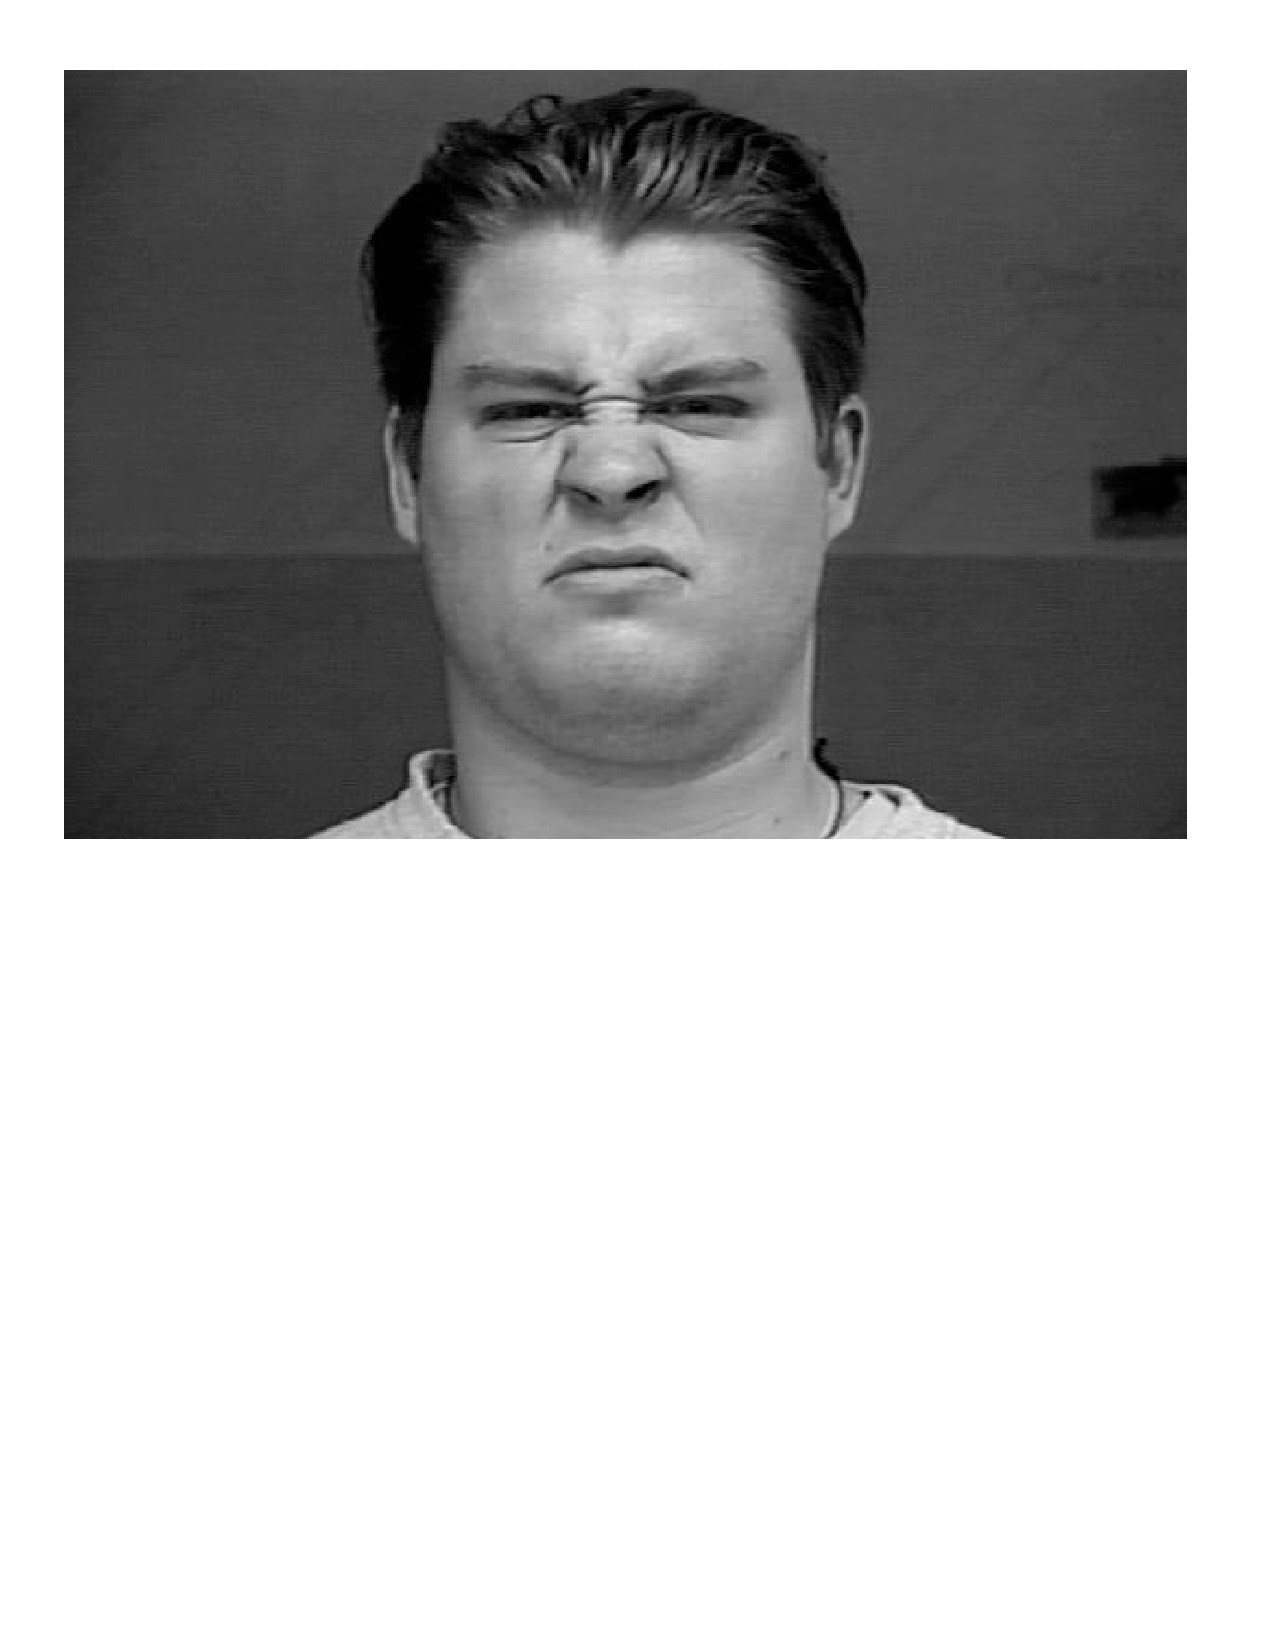
\includegraphics[width=\textwidth]{ME31}
      \caption{}
    \end{subfigure}%
    ~%add desired spacing
    \begin{subfigure}[b]{0.22\textwidth}
      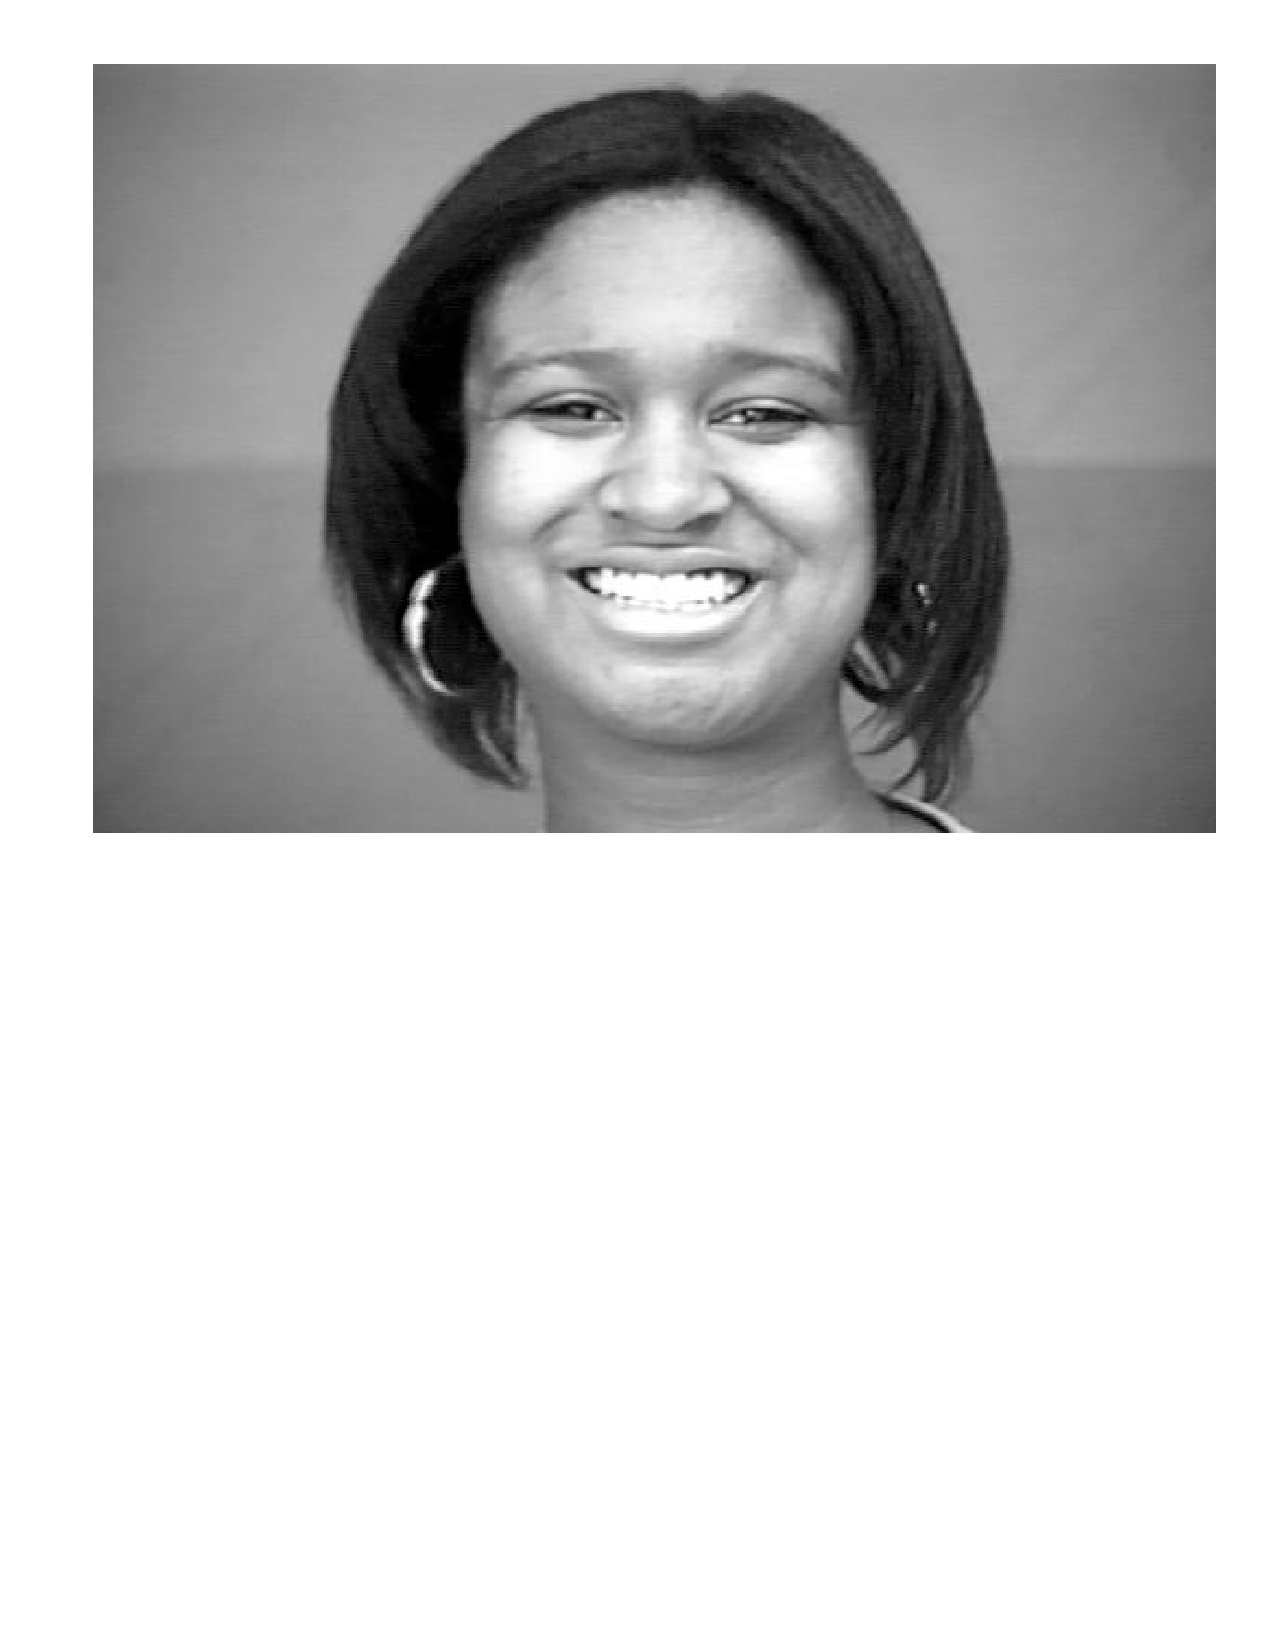
\includegraphics[width=\textwidth]{ME32}
      \caption{}
    \end{subfigure}
    \begin{subfigure}[b]{0.22\textwidth}
      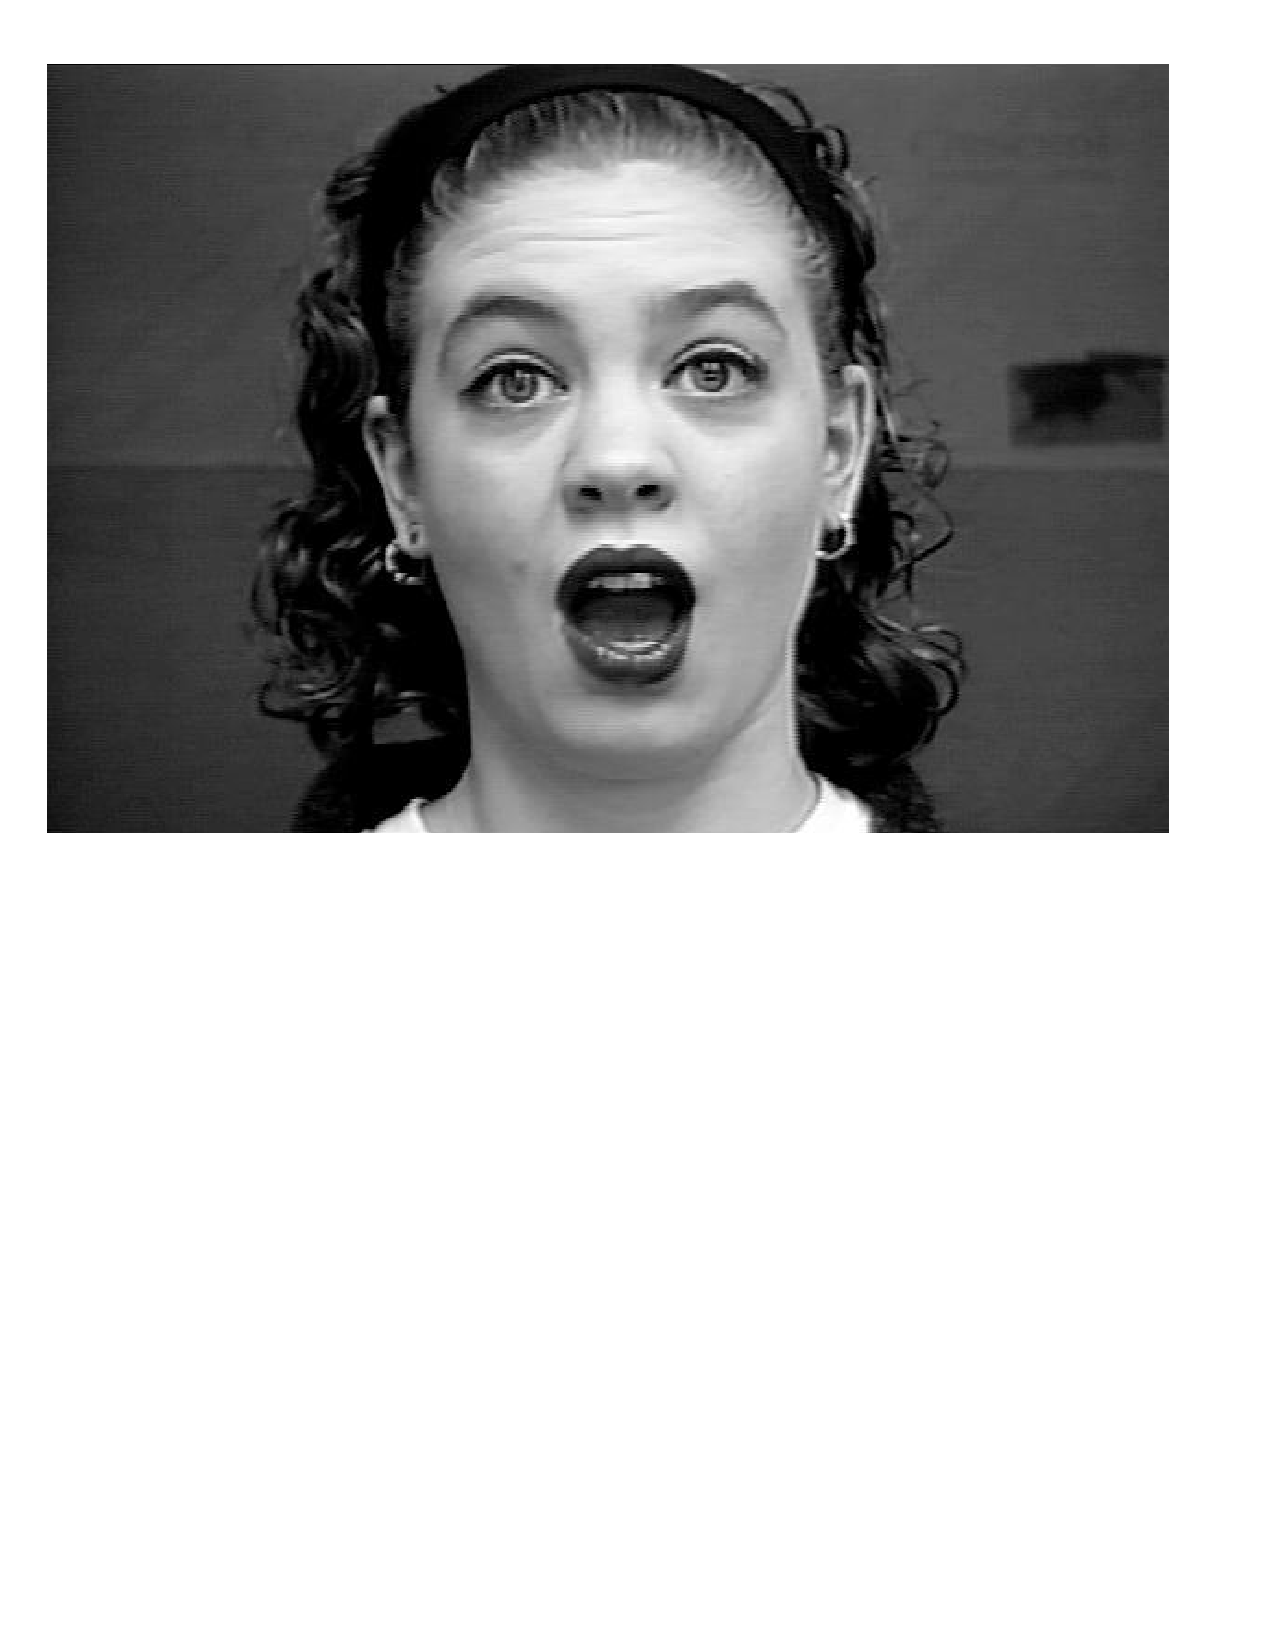
\includegraphics[width=\textwidth]{ME33}
      \caption{}
    \end{subfigure}%
    ~%add desired spacing
    \begin{subfigure}[b]{0.22\textwidth}
      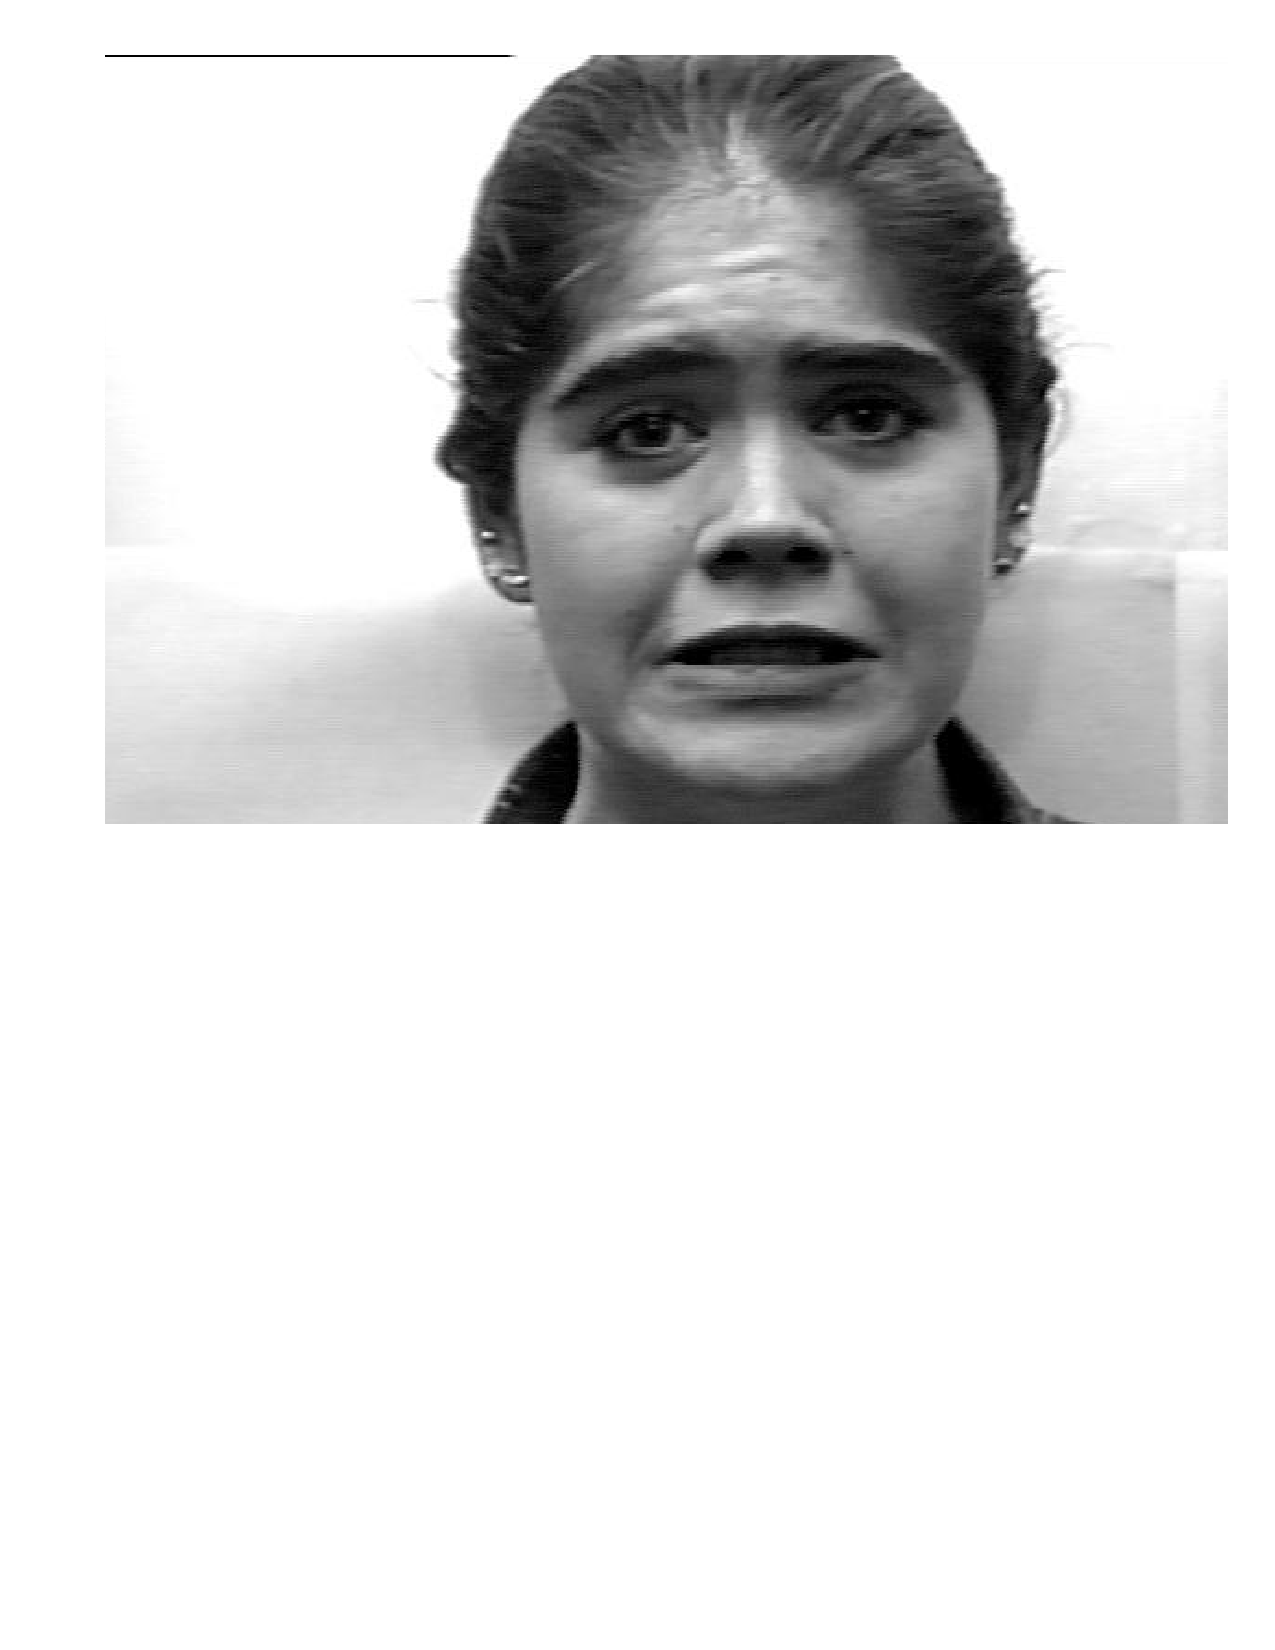
\includegraphics[width=\textwidth]{ME34}
      \caption{}
    \end{subfigure}
    \begin{subfigure}[b]{0.22\textwidth}
      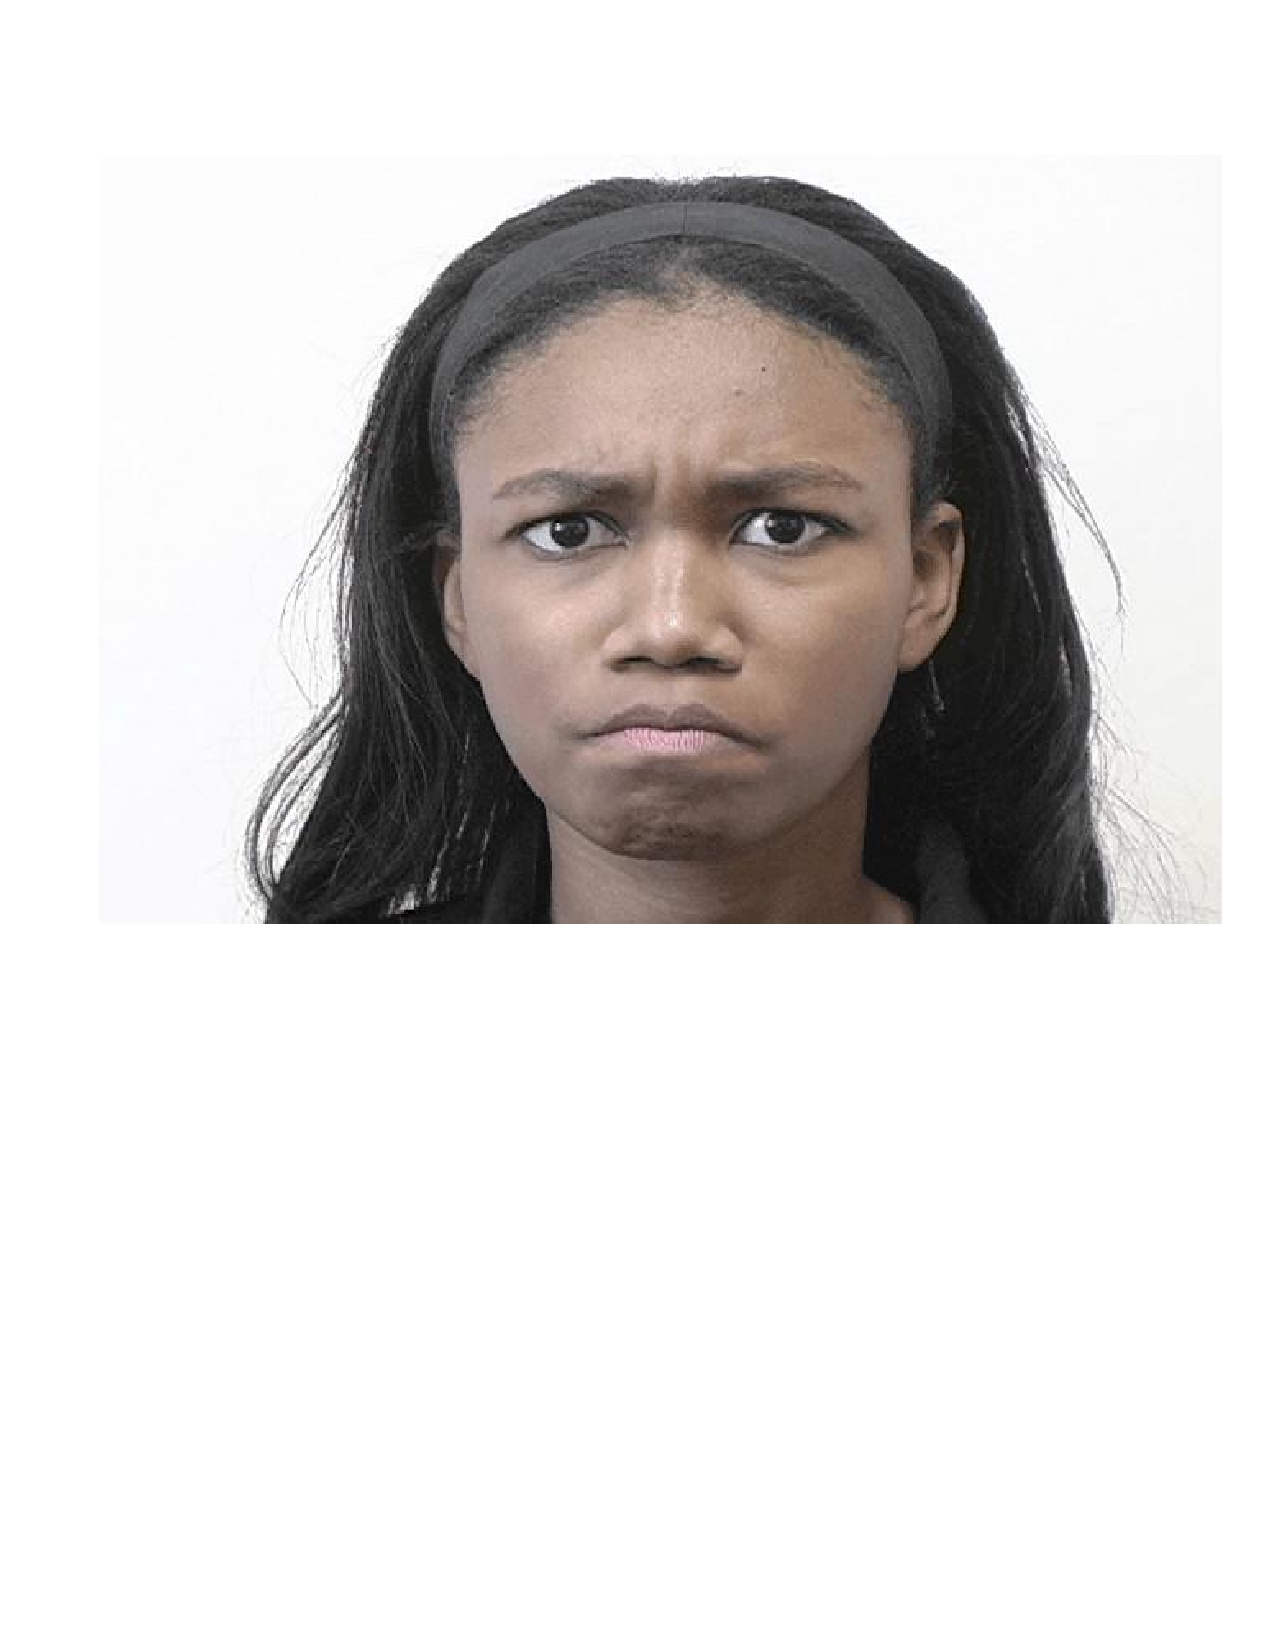
\includegraphics[width=\textwidth]{ME35}
      \caption{}
    \end{subfigure}
    \begin{subfigure}[b]{0.22\textwidth}
      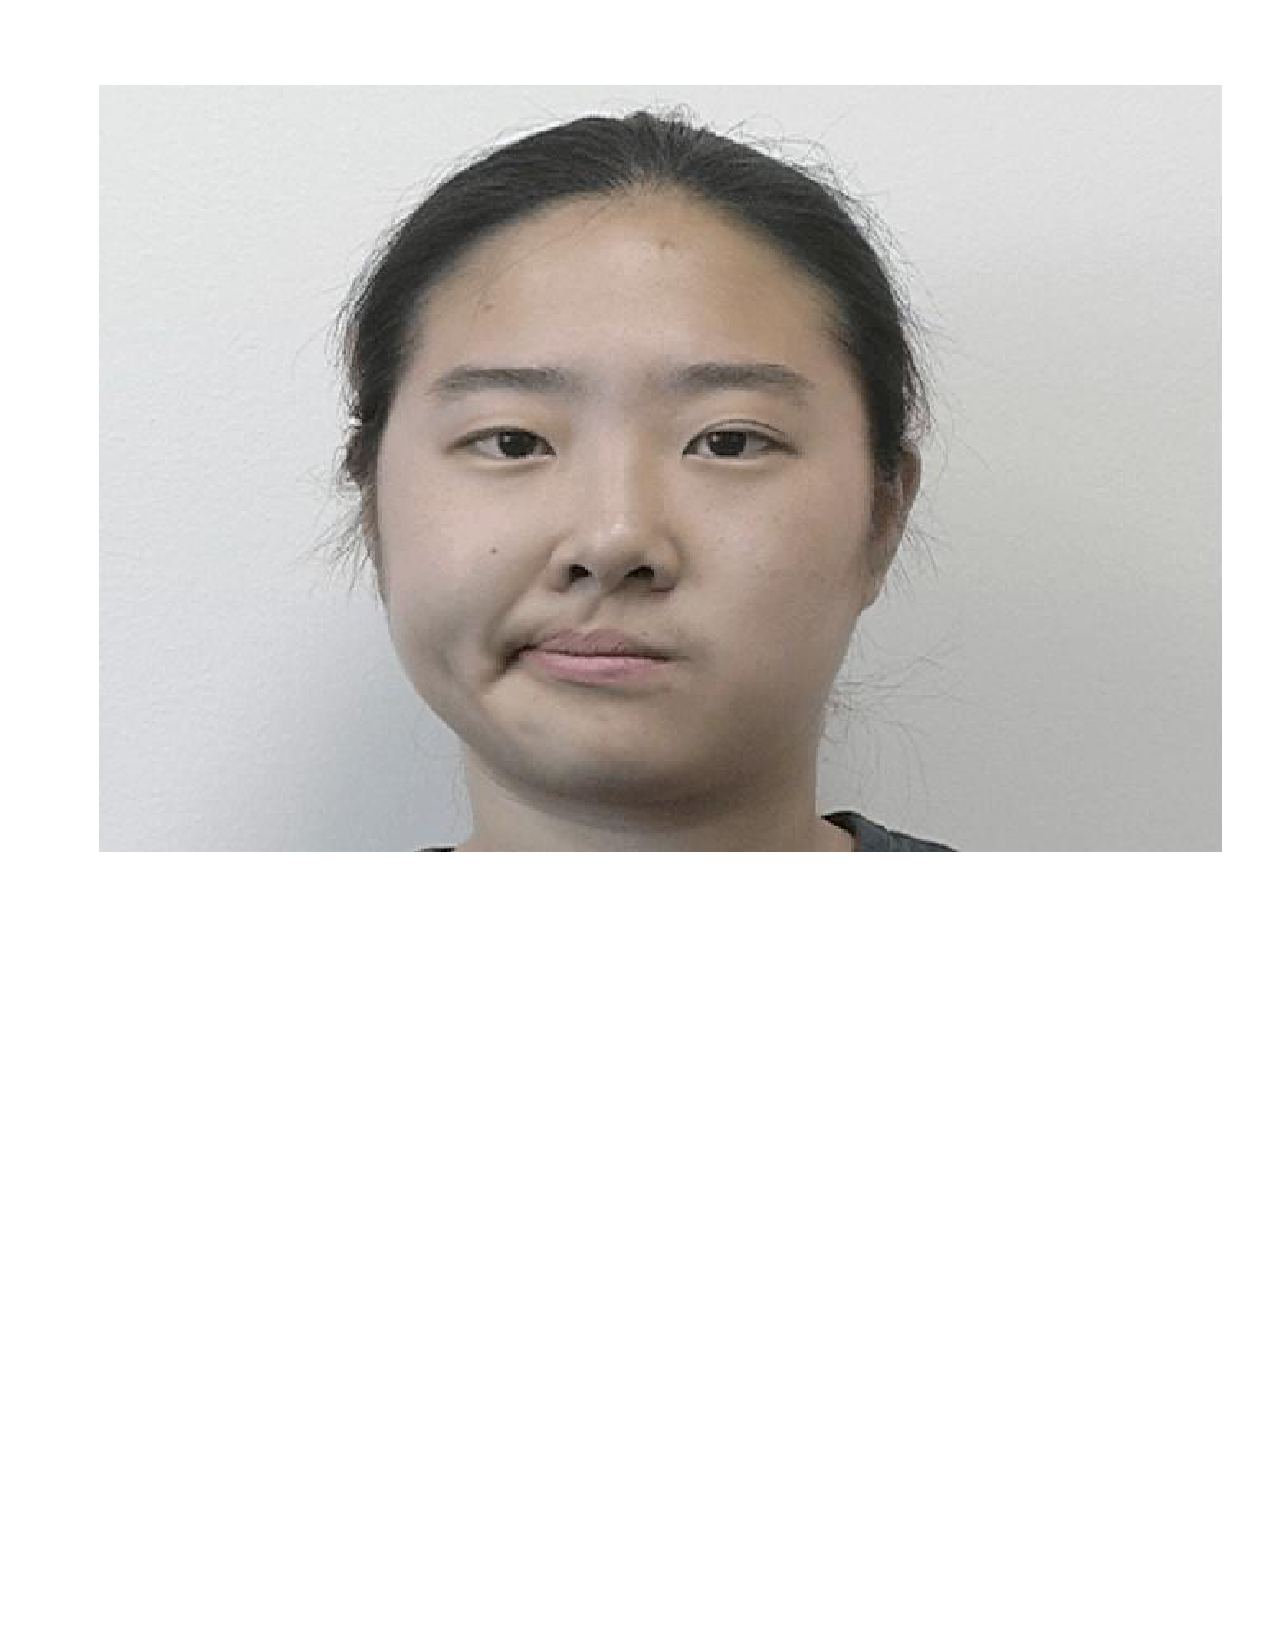
\includegraphics[width=\textwidth]{ME36}
      \caption{}
    \end{subfigure}
    \begin{subfigure}[b]{0.22\textwidth}
      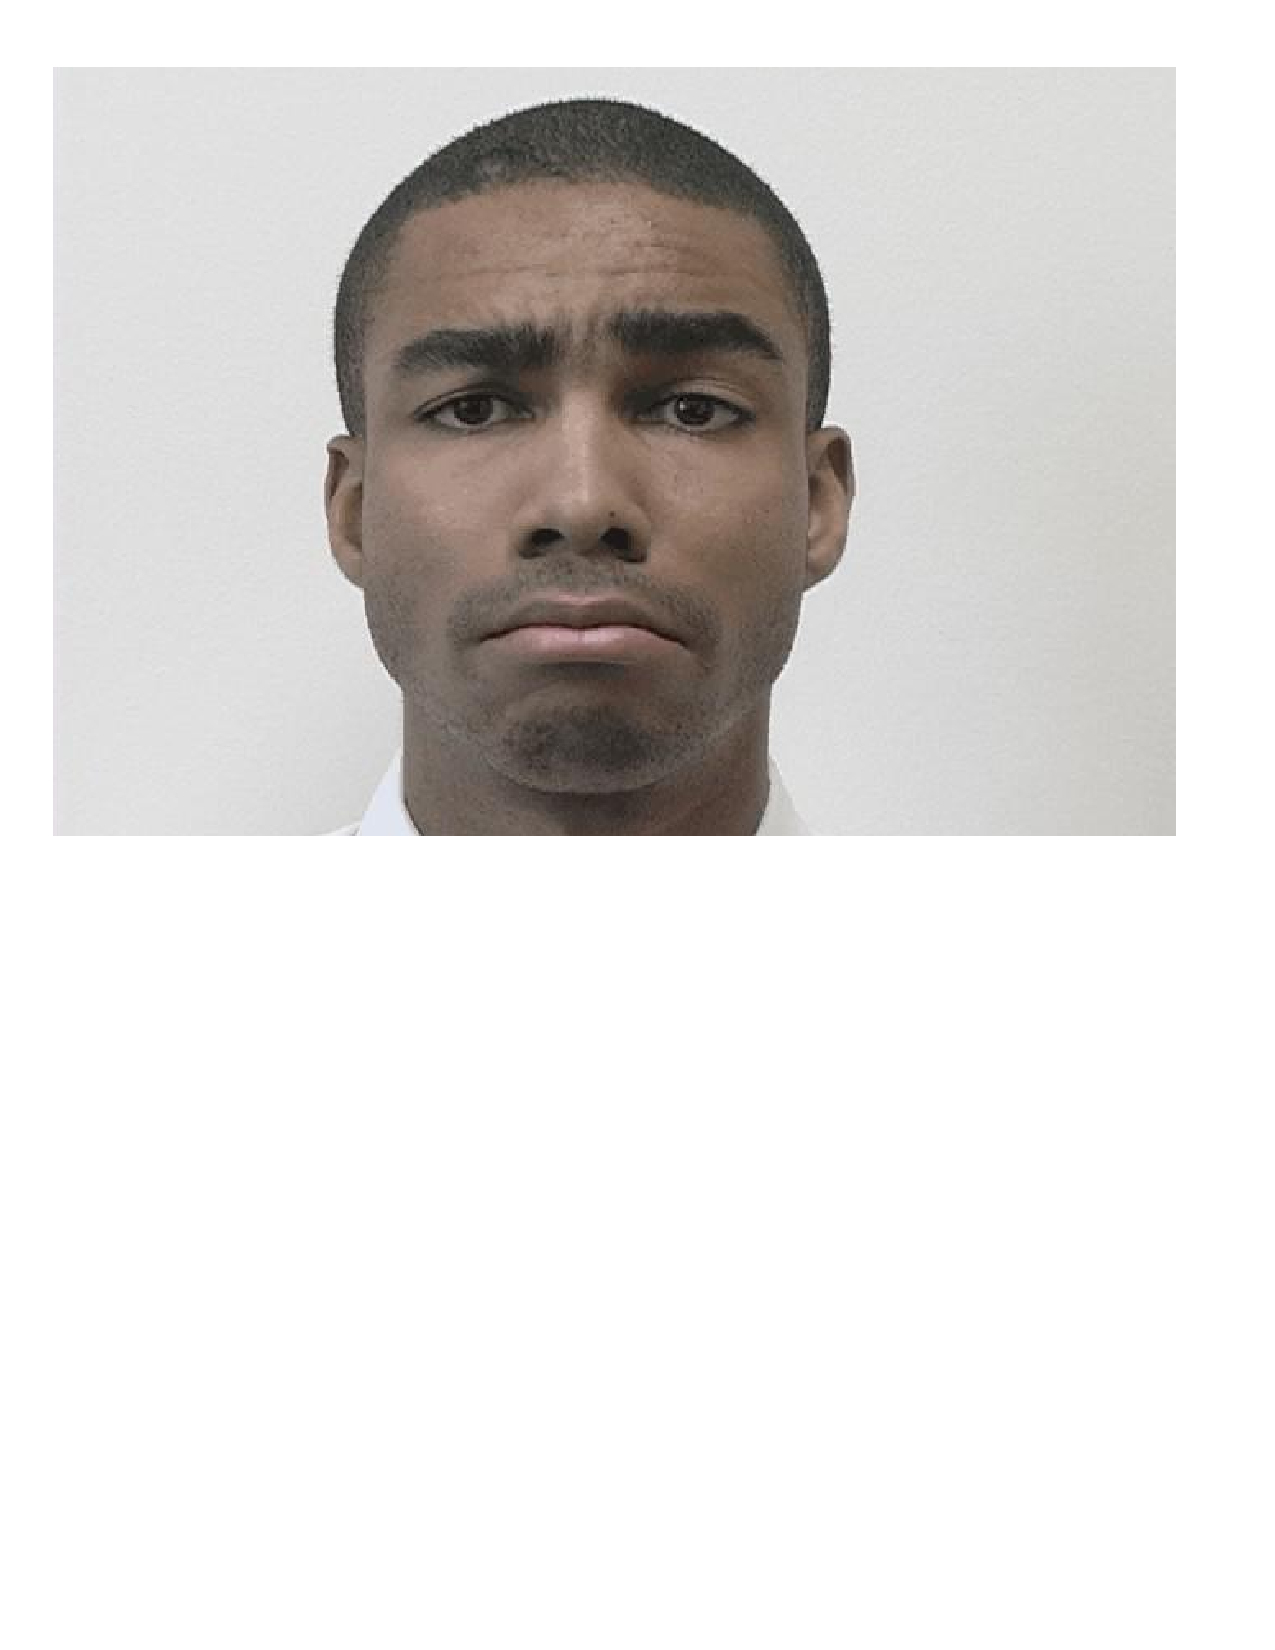
\includegraphics[width=\textwidth]{ME37}
      \caption{}
    \end{subfigure}
    \begin{subfigure}[b]{0.22\textwidth}
      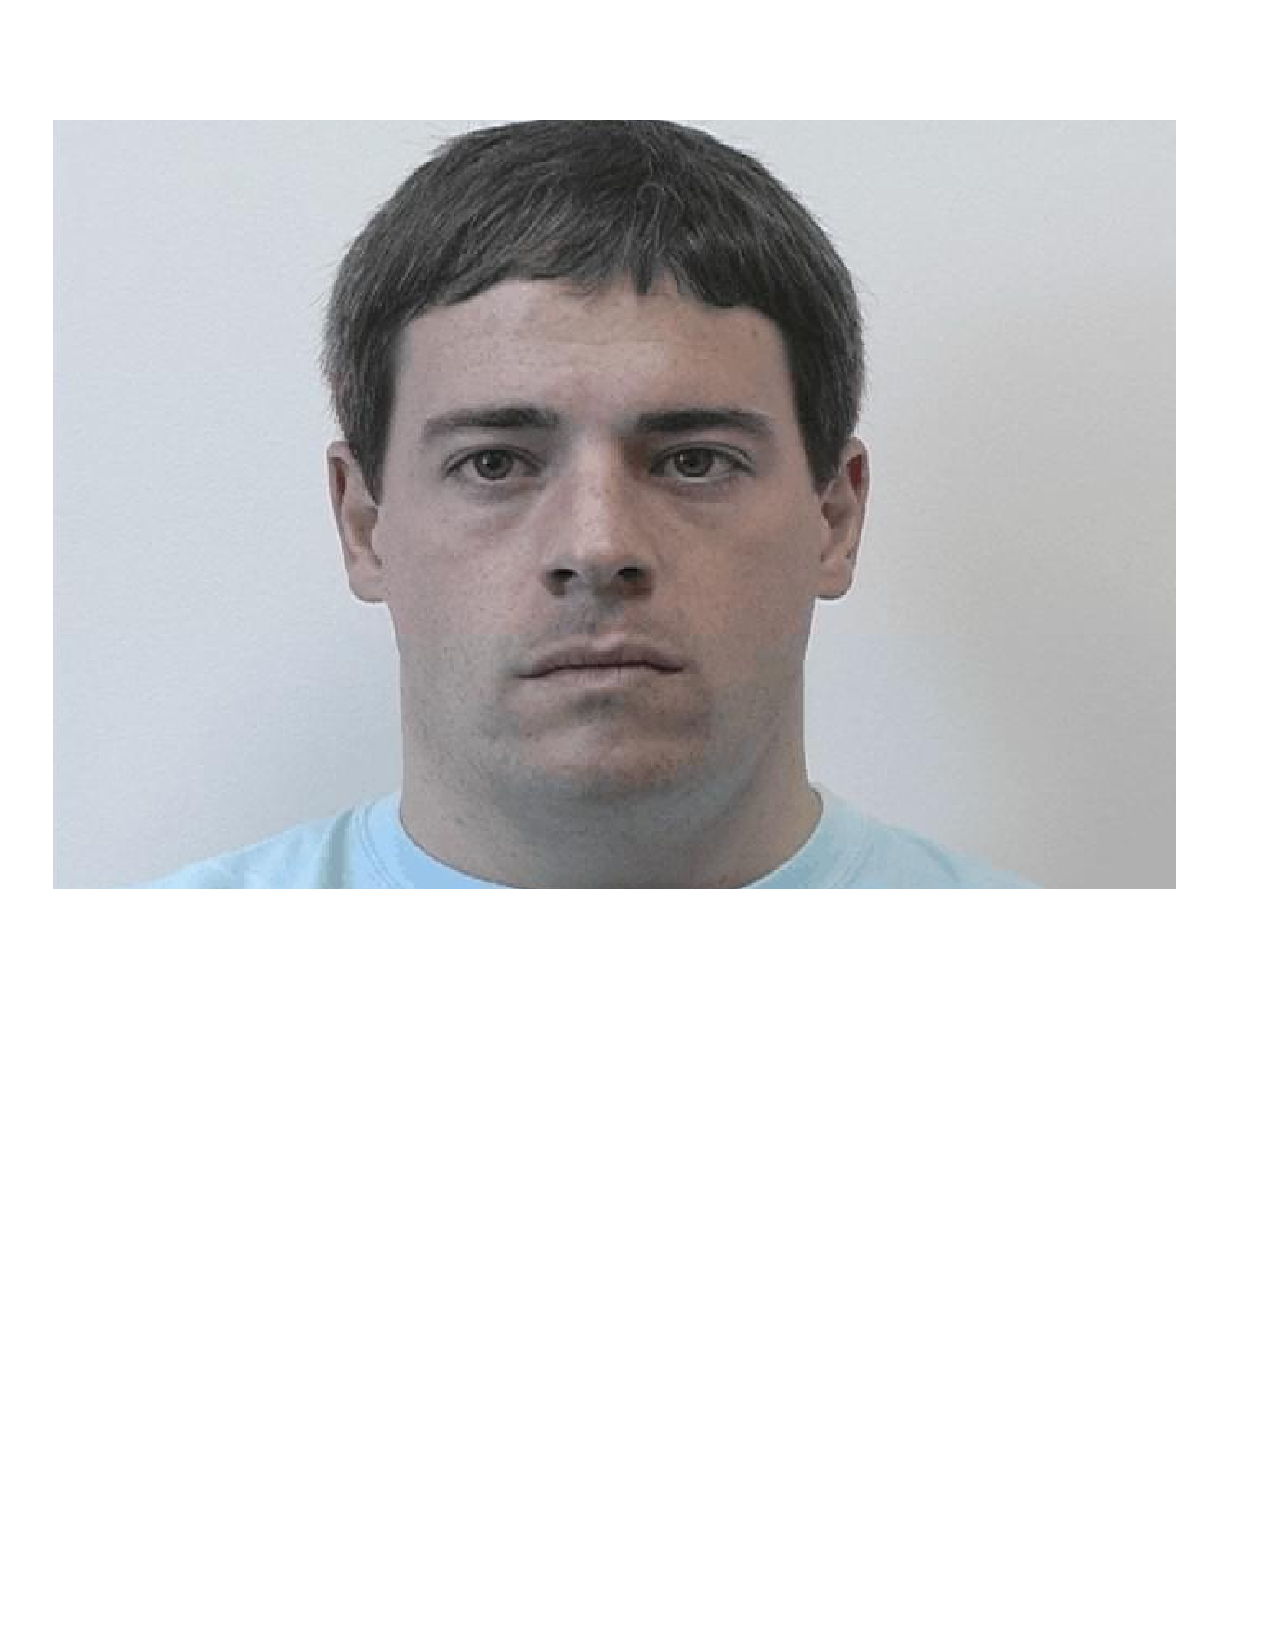
\includegraphics[width=\textwidth]{ME38}
      \caption{}
    \end{subfigure}
    \caption{人脸宏表情样本示例\\ \footnotesize \textmd{(a)厌恶、(b)快乐、 (c)惊讶、(d)恐惧、(e)愤怒、(f)轻蔑、(g)沮丧、(h)中性表情}}
    % \caption{人脸宏表情样本示例(CK+数据集)\\ \footnotesize \textmd {}(a)厌恶、(b)快乐、 (c)惊讶、(d)恐惧、(e)愤怒、(f)轻蔑、(g)沮丧、(h)中性表情}}
    % \caption{\footnotesize \textmd{(a)厌恶、(b)快乐、 (c)惊讶、(d)恐惧、(e)愤怒、(f)轻蔑、(g)沮丧、(h)中性表情}}
    \label{fig1}
\end{figure}

\subsection{早期微表情数据集}

由于微表情在镜头下很难产生,所以微表情数据的缺乏是微表情研究的第一障碍。虽然微表情已经被心理学家研究了很长一段时间,但网络上广泛传播的微表情样本仅仅只有片段,并没有发现任何心理学研究小组分享的大数据集。作者认为第一个原因是心理学研究更关注微表情本身的性质,比如什么时候出现或者看起来是什么样子,所以他们不需要像使用计算机研究那样需要大量的微表情数据。其次,在某些情况即使涉及到大量的微表情数据,但由于保密性限制,数据无法公开共享,例如患者的病历或司法讯问记录等。

以2009年为时间点,在此以前属于微表情的早期研究阶段,一些研究人员在他们的研究中使用了摆拍的微表情数据,这些数据避免了自发微表情数据获取时的困难,作为早期自动微表情识别研究的尝试,使用摆拍的数据是一次历史性的突破。例如Shreve等人收集了一个名为USF-HD的数据集,其中包含100个摆拍的微表情片段,视频长度平均在1分钟左右,最长2分钟,最短20秒。研究人员要求参与者模仿屏幕上显示的微表情样本作为数据的来源,同时在他们的文章中明确写到可以通过要求参与者尽可能快地模仿来收集一个摆拍的微表情数据集。Polikovsky等人也收集了一个摆拍的微表情数据集,要求受试者在低强度下表演七种基本情绪,并尽快回到中性表情,数据由一台每秒200帧的高速摄像机记录。表~\ref{tab3}列出了摆拍的微表情数据集的详细属性。

\begin{table}[!htbp]
\centering
\caption{摆拍微表情数据集}
\label{tab3}
\footnotesize% fontsize
\setlength{\tabcolsep}{5pt}% column separation
\renewcommand{\arraystretch}{1.2}%row space
\begin{tabular}{c|cc}
\hline
 & USF-HD & Polikovsky \\ \hline
微表情片段 & 100 & N/A \\
参与者 & N/A & 10 \\
分辨率 & $720\times1280$ & $480\times640$ \\
FPS & 29.7 & 200 \\
FACS & NO & YES \\
表情类 & N/A & 7 \\
人种 & N/A & 3 \\ \hline
\end{tabular}
\end{table}

值得注意的是摆拍的微表情数据不可以代替或与自发的微表情数据一起使用,因为这两种数据是不同性质的。例如在研究微表情的起始点时,由于两者是在不同的机制下产生的,所以摆拍的微表情在时空特性上与自发的微表情存在很大的差异,其次在研究视频的上下文时,由于模仿的表情与通过视频编辑生成的摆拍微表情片段通常在起止点很突兀,而且期间禁止其他无关的动作发生,这也与自发的微表情有很大的不同。另一方面,自然环境下自发的微表情可能伴随着复杂的场景,比如头部运动和眨眼等动作。基于这些事实,利用摆拍的微表情数据进行研究并不能真正解决实际中微表情分析的自动化问题,所以努力收集自发的微表情数据是后续工作的正确路径。需要说明的是在本文接下来的内容中,所有的工作都是关于自发微表情的,如果没有特别说明,“微表情”一词表示自发微表情。

\subsection{自发微表情数据集}

A. SMIC数据集介绍

2011年,论文\citepns{pfister2011recognising}首次提出了一种诱导和收集自发微表情的方法,将获得的数据集命名为“自发微表情语料库”,简称SMIC,它是第一个使用自然诱发状态的微表情数据集,对后续的数据集建立具有很好的指导性意义。第一版的SMIC数据集只包含了6位参与者的数据,论文\citepns{Li2013A}对其进行了扩充,包含了16名参与者的164个自发微表情片段,由三种相机记录的3个数据集组成:100fps的高速相机记录的HS数据集、25fps的普通彩色相机记录的VIS数据集和25fps的近红外摄像机记录的NIR数据集,且所有数据集具有相同的图像分辨率$640\times480$。增加VIS和NIR摄影机有三个考虑:(1)提升数据集的多样性;(2)研究高速相机在微表情分析方面是否优于普通速度相机;(3)研究时间插值方法是否可以应用于普通高速相机,以解决相机的短时插值问题。图~\ref{fig2}给出一个消极的微表情序列,通过该样例可以看出,一个微表情是由一组图片序列构成的,本样例的变化主要表现为嘴角的细微下沉。
\begin{figure}[!htbp]
    \centering
    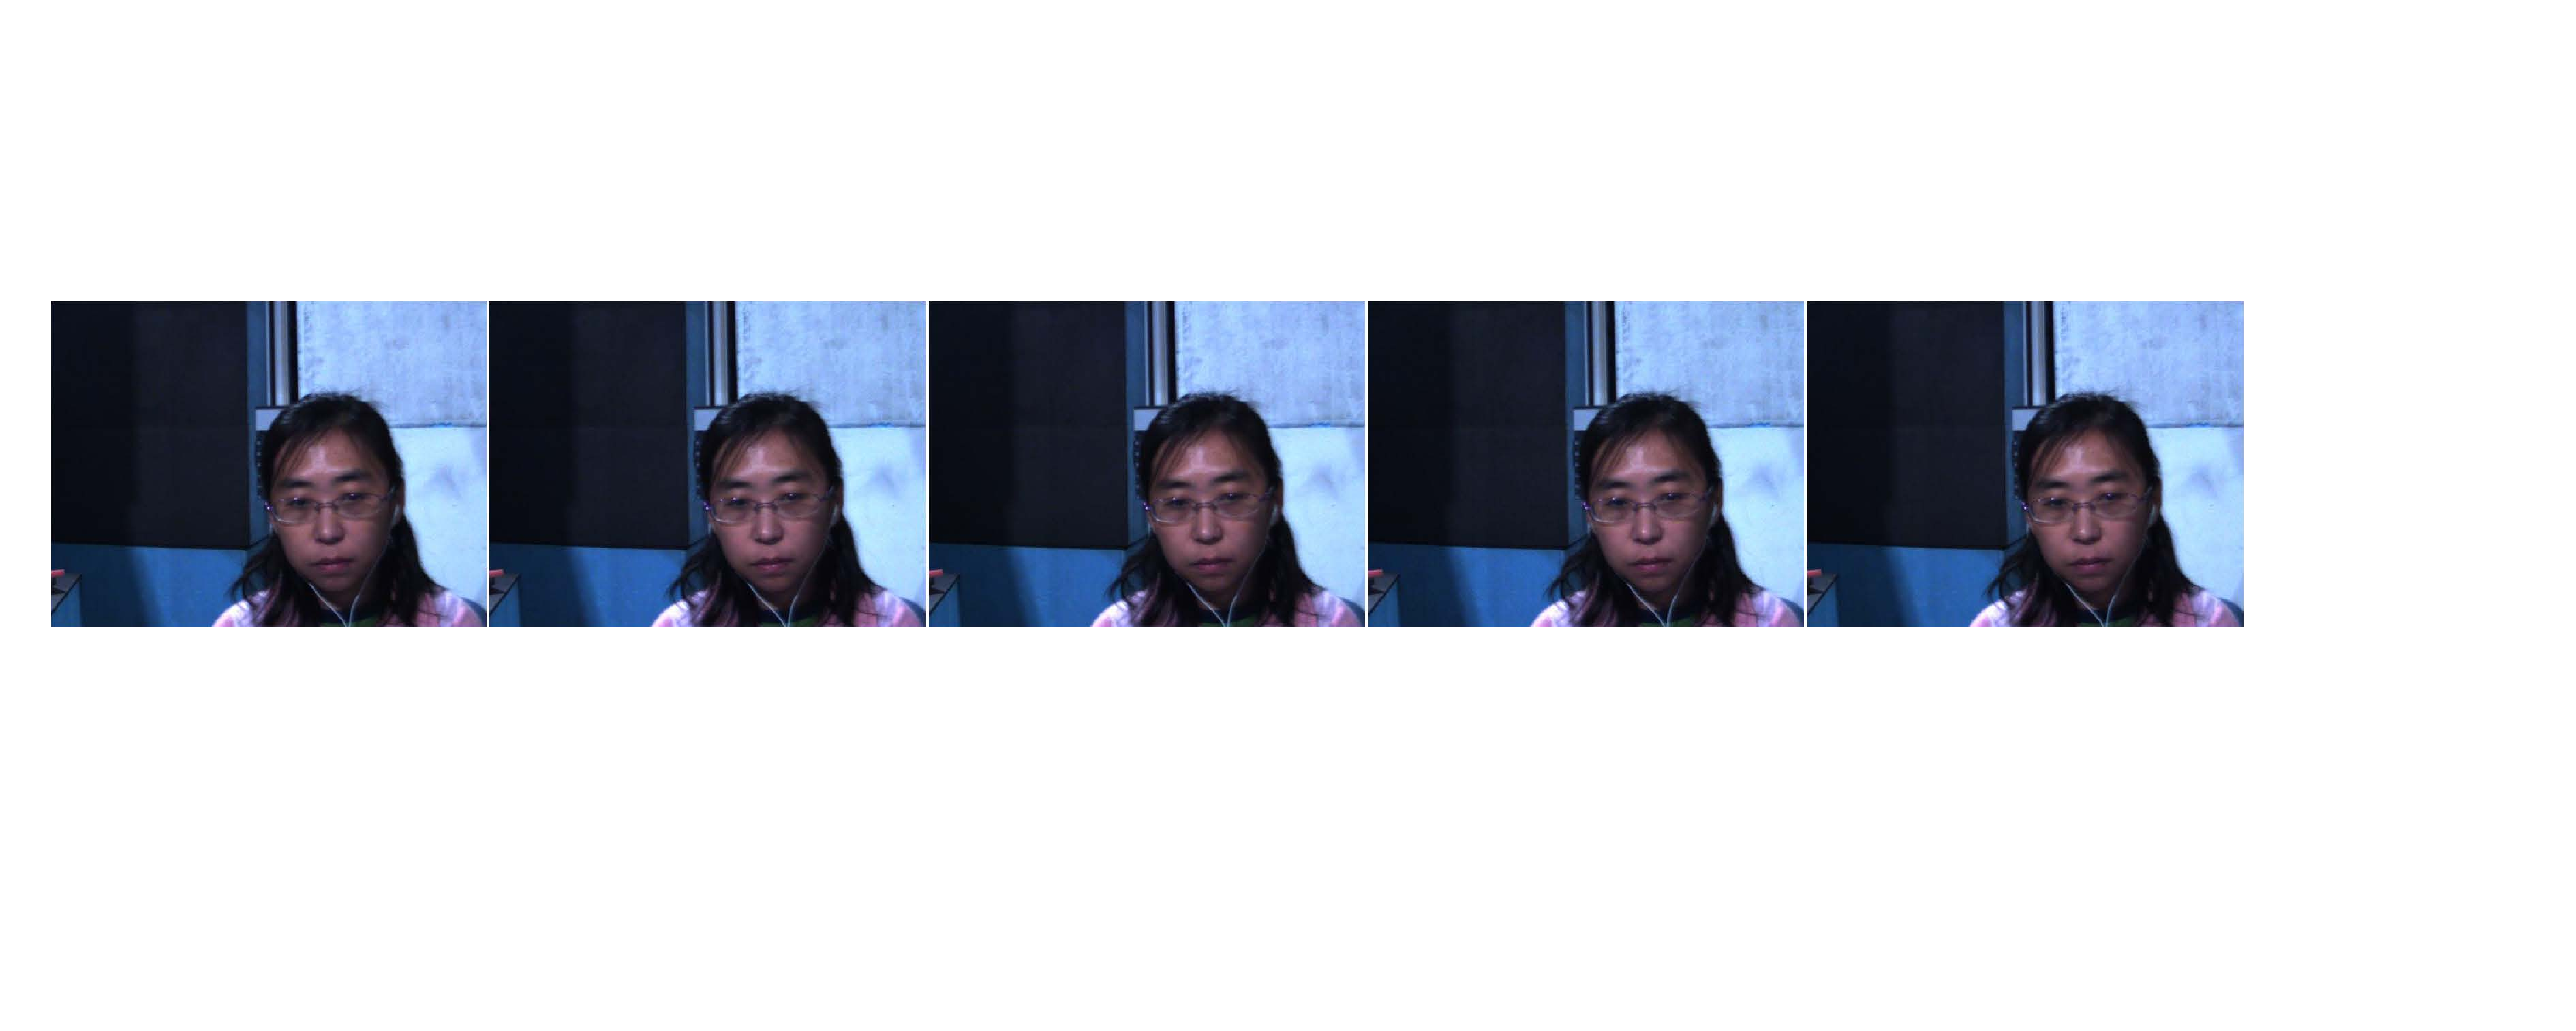
\includegraphics[width=0.95\textwidth]{ME1}
    \caption{一个消极的微表情片段示例(SMIC数据集)}
    \label{fig2}
\end{figure}

a)视频采集

研究表明通过图像、视频和音乐等一定的刺激能够诱发真实的表情\citep{Coan2015Handbook}。自发微表情是由人的内心感受触发的非自愿行为,所以可以使用上述方法引发情感反应。但必须找到一种能确保诱发的表情足够短的方法(满足微表情的标准)。一些心理学著作研究了微表情发生的条件,Ekman等人认为当人们试图隐藏自己的真实情感时,尤其是当被抓住后果会很严重时,微表情就会出现,这被称为高风险条件,例如嫌疑人正在接受警察或测谎专家的审问,这是一种很自然的高风险场景。但是对于采集数据而言,营造真正的审问现场显的不太可能。所以为了诱导参与者自发的微表情,需要找到一种模拟高风险环境的方法。设计的情景必须满足以下两个要求:(1)激发参与者情绪的刺激必须有效,使激发的情绪反应强烈到无法完全隐藏;(2)应该制造高压力,这样参与者才会有动力去尽力隐藏自己的真实感受。

作者使用了心理学研究中诱导抑制情绪产生的方法。采集前向参与者详细说明研究内容和过程,显示器上显示如下提示性语句:“(1)将向您展示几段诱发情绪的短片,请尽量保持头部稳定并仔细观看。(2)每段视频片段后,您将有一个短暂的休息。请根据您对刚才看到的视频的真实感受填写调查表(报告中的情感反馈是标注过程中的重要参考。)。(3)当您在看视频的时候,我会待在另一个房间,通过摄像头观察您的面部和身体动作,并尝试猜测您所看的视频片段(片段是随机播放的)。您的任务是装出若无其事的样子,而不是表露您的真实感情。如果您不能隐藏您的感觉,您将不得不填写一份超过500个冗长而乏味的问题问卷。”

在每段影片结束后,参与者将在问卷中回答以下问题:“(1)您在看视频时感受到了什么样的情绪(快乐、悲伤、厌恶、恐惧、惊讶、愤怒或困惑)?(2)看视频的时候您是否感觉到愉悦?(从1到7愉悦程度逐渐上升)”。选择最有效的刺激作为情感诱导因子是后续数据采集的关键因素之一。通过查阅文献比较不同类型的情绪诱导材料,如图像、音乐、视频和互动。最终决定使用短视频作为微表情采集诱导剂的原因有三个:(1)视频包含音频和视觉信息,因此比图像和音乐的影响更强大;(2)视频能够持续一段时间,更能激发强烈情绪,更容易产生微表情;(3)从获取稳定额叶面部视频的实际角度来看,观看视频的参与者比多人参与的互动场景更容易控制。

20名来自奥卢大学的学生和研究人员自愿参与数据集的制作,参与者的年龄从22岁到34岁不等,其中7位是女性,13位是男性,9人是白种人,11人是亚洲人。研究人员在电脑显示器上向参与者展示了16段精心挑选的能引发强烈情绪的视频片段。当参与者观看视频片段时,三个固定在电脑显示器上的摄像头记录参与者的面部反应,操作人员在前方通过另外一台电脑监控参与者的面部反应,图~\ref{fig3}给出了环境设置示意图。

\begin{figure}[!htbp]
    \centering
    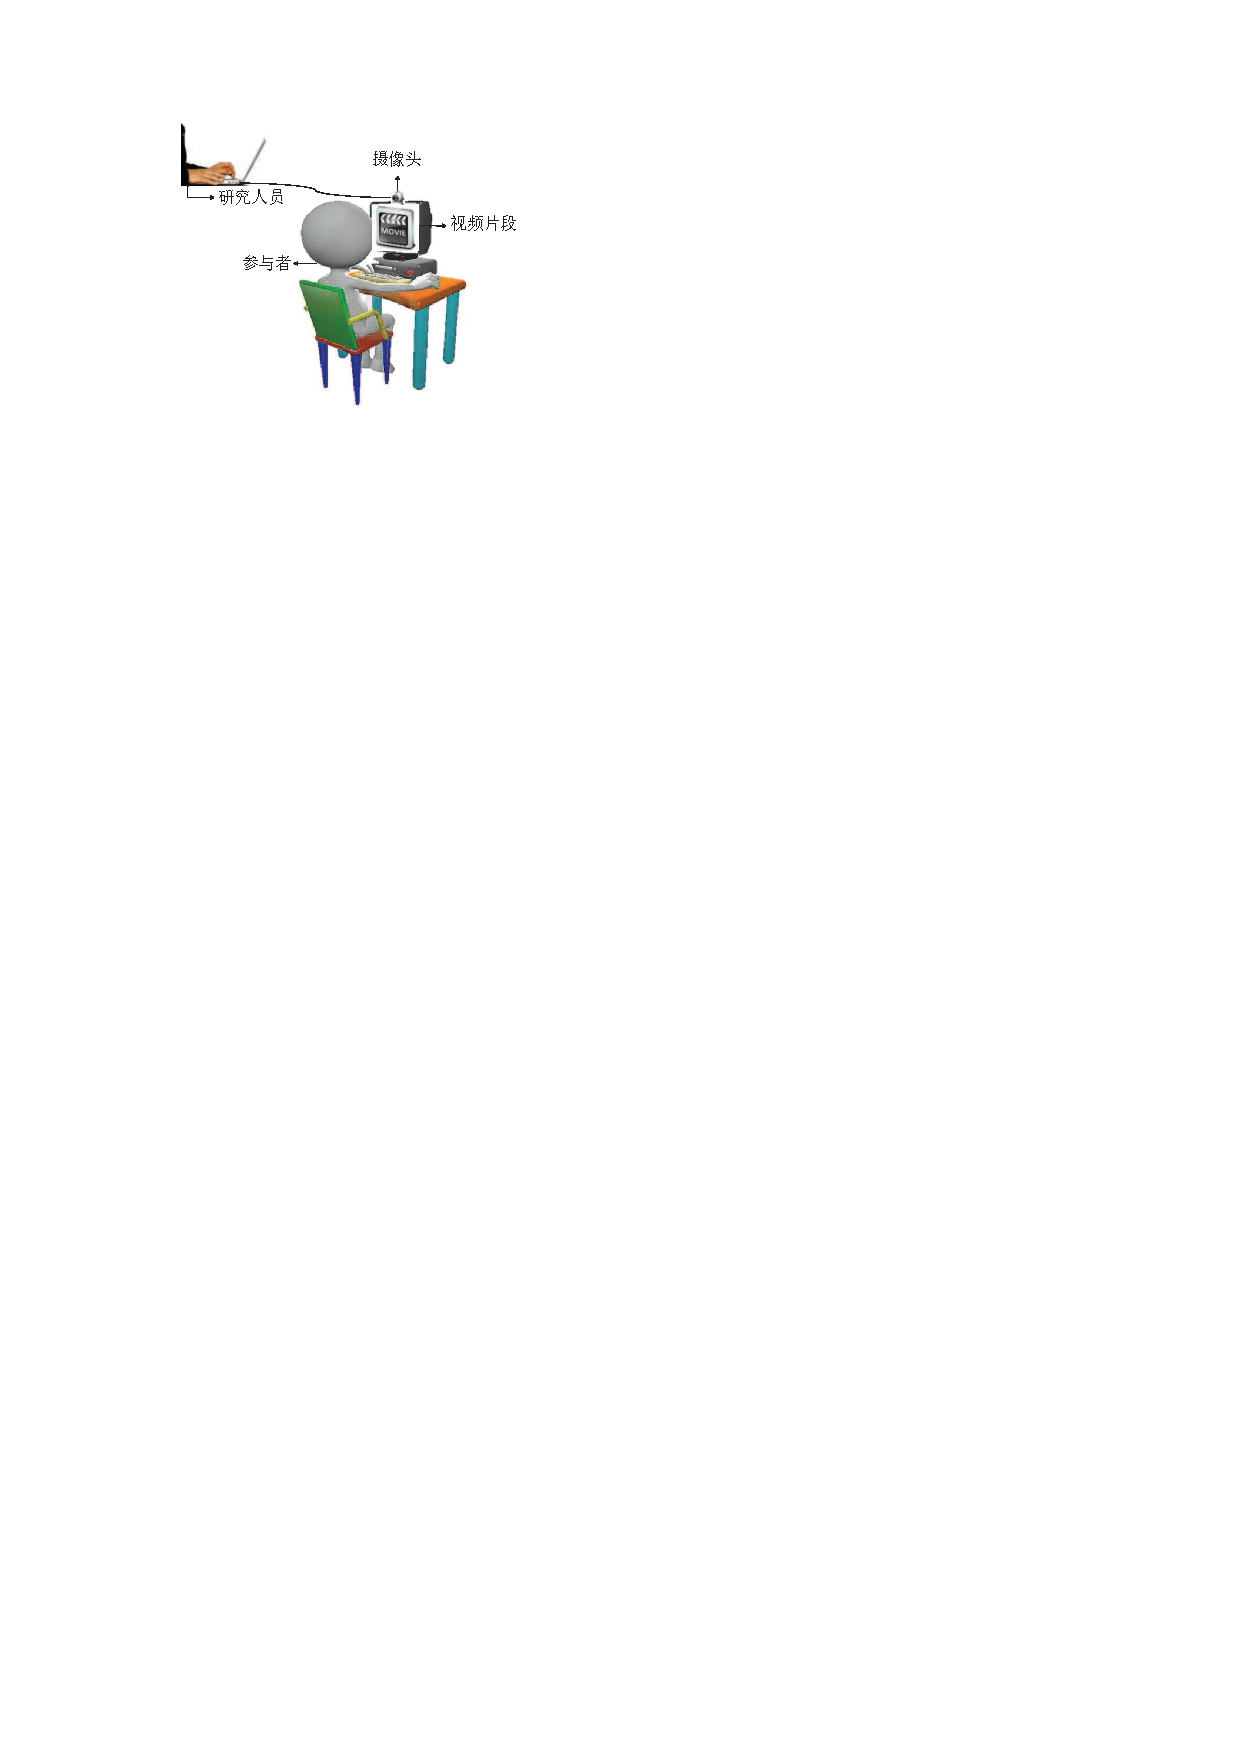
\includegraphics[width=0.45\textwidth]{collect}
    \caption{微表情数据采集示意图}
    \label{fig3}
\end{figure}

b) 视频的标注

录制的视频需要进行分割和标注,目的是得到适合研究人员进行训练与测试的微表情样本和相应的标签。采集的三种视频中高速视频由于具有最佳的时间分辨率所以非常适合标注,另外两个摄像头拍摄的视频需要同步后再进行标注。首先,从原始的长视频中分割出微表情的起始和终止帧,微表情序列的开始表示的是与之前中立(或接近中立)的人脸表情相比的可见运动的第一帧,而微表情序列的终止指在与下一帧相比可以发现任何运动时结束的最后一帧。关于微表情精确的长度限制目前还存在争议,SMIC数据集参考论文\citepns{Yan2013How}和 \citepns{matsumoto2011evidence}等人的建议,设置了1/2秒较宽松的分割节点。注意,并不是所有的微表情都结束于一个完全的中性表情,有些表情可能会上升,然后下降到接近中性的状态,并保持这种状态很长时间,这也被认为是微表情的结束。

随后,对所有的视频片段都用情感标签进行标注。情感标签的证据有两种:视频片段的内容和参与者提交的报告。虽然在视频播放前已经预知将可能产生某种确定情绪,但研究发现,参与者在某些视频刺激下可能会产生不同的情绪表现(甚至相反的情绪)。在少数情况下,当参与者提交的问卷报告与视频内容相反时(例如,一些参与者反馈在观看恐怖视频片段时感到快乐或有趣),SMIC数据集使用参与者的提交的报告作为微表情标签的标准。起初,SMIC数据集根据视频内容分配了五种情感标签,包括快乐,悲伤,恐惧,厌恶,惊讶。后来,SMIC数据集将五类标签合并为三类:积极(Positive)、惊喜(Surprise)和负面(Negative)。将第一版本的快乐类别改为新的积极类别,而消极类别则是由第一版的悲伤、恐惧和厌恶这三个类别组合而成。将三种消极情绪融合在一起的原因是:首先,参与者在该段视频的报告中选择了三种情绪中的一种以上;其次,三种标签的样本量都太小,合并后会更好的平衡。根据具体情况,惊喜类别可以分为正面惊喜和负面惊喜。同时为了验证数据标签的有效性,标注由两位标注者分别执行。然后,两位标注者相互交换检查各自的标注,只有当两位标注者的标注结果一致时的标签有效。

B. CASMEC数据集介绍

在SMIC发表后不久,另一组研究人员收集了新的自发微表情数据集。由中国科学院Yan等人采用与SMIC相似的情绪诱导方式收集了中国科学院微表情数据集(CASME),包含19位中国籍参与者的195个微表情片段。CASME由两台相机记录,一台是明基M31相机,帧率为60fps,分辨率为$1280\times720$(CASME-A),另一台是灰点GRAS-03K2C相机,帧率为60fps,分辨率为$640\times480$(CASME-B)。CASME数据集中的微表情首先使用AU标记,然后被分为八类情绪,包括娱乐、悲伤、厌恶、惊讶、蔑视、恐惧、压抑和紧张。之后又发布了第二版数据集CASME II,CASME II提供了更多具有更高时空分辨率的微表情样本。新数据集的平均人脸尺寸为$280\times340$,每秒200帧,是从26名中国参与者中获得的247个微表情样本。CASMEII样本有五个类的AU标签和情感标签,即幸福、厌恶、惊讶、压抑和其他。

CASME II数据集相比之前的数据集引入了AU标签,它是在充分考虑了主客观因素(除了FACS编码的基本判断)外,还参考了参与者自己的主观回忆来辅助标注的样本标签。除此之外,该数据集还对微表情的起始帧、峰值帧和终止帧都做了详细的标注。

C. 其他数据集介绍

最近又有一个新的自发微表情数据集SAMM发布,它也使用了类似于SMIC和CASME的情绪诱导方法,从13个不同民族的32名参与者中获得159个微表情。SAMM数据具有更高的帧分辨率$2040\times340$,帧速率为200fps。数据提供了AU标签和七种表情标签,包括生气、开心、蔑视、恐惧、惊讶、厌恶和其他。

表~\ref{tab1}列出了当前所有提到的微表情数据集的详细参数。

\begin{table}[!htbp]
  \centering
  \caption{自发微表情数据集}
  \label{tab1}
  \footnotesize% fontsize
  \setlength{\tabcolsep}{4pt}% column separation
  \renewcommand{\arraystretch}{1.2}%row space
  \begin{tabular}{c|cccccc}
    \hline
     & SMIC-HS & SMIC-subHS & SMIC-NIR & SMIC-VIS & CASME II & SAMM \\ \hline
    微表情片段 & 164 & 71 & 71 & 71 & 247 & 159 \\
    参与者 & 16 & 8 & 8 & 8 & 26 & 32 \\
    分辨率 & $640\times480$ & $640\times480$ & $640\times480$ & $640\times480$ & $640\times480$ & $2040\times1088$ \\
    人脸分辨率 & $190\times230$ & $190\times230$ & $190\times230$ & $190\times230$ & $280\times340$ & $400\times400$ \\
    FPS & 100 & 100 & 100 & 100 & 200 & 200 \\
    性别比(F/M) & 6/10 & 2/6 & 2/6 & 2/6 & 15/11 & 16/16 \\
    FACS & NO & NO & NO & NO & YES & YES \\
    表情类 & 3 & 3 & 3 & 3 & 5 & 7 \\
    平均年龄(SD) & 26.7(N/A) & 26.7(N/A) & 26.7(N/A) & 26.7(N/A) & 22.03(SD=1.6) & 33.24(SD=11.32) \\
    人种 & 2 & 2 & 2 & 2 & 1 & 4 \\ \hline
    \end{tabular}
\end{table}

\subsection{宏表情与微表情比较}

通过前两小节的介绍可以看出微表情和宏表情最大的区别是在面部肌肉的运动强度和持续时间。如图~\ref{fig4}所示,人脸根据不同的部位被划分为不同的肌肉组如皱眉肌、降眉间肌、鼻肌等,图~\ref{fig1}中上述肌肉运动明显比图~\ref{fig2}更加剧烈也更加夸张;另一方面,微表情的持续时间一般在1/25秒到1/2秒之间,而宏表情则不然。

\begin{figure}[!htbp]
    \centering
    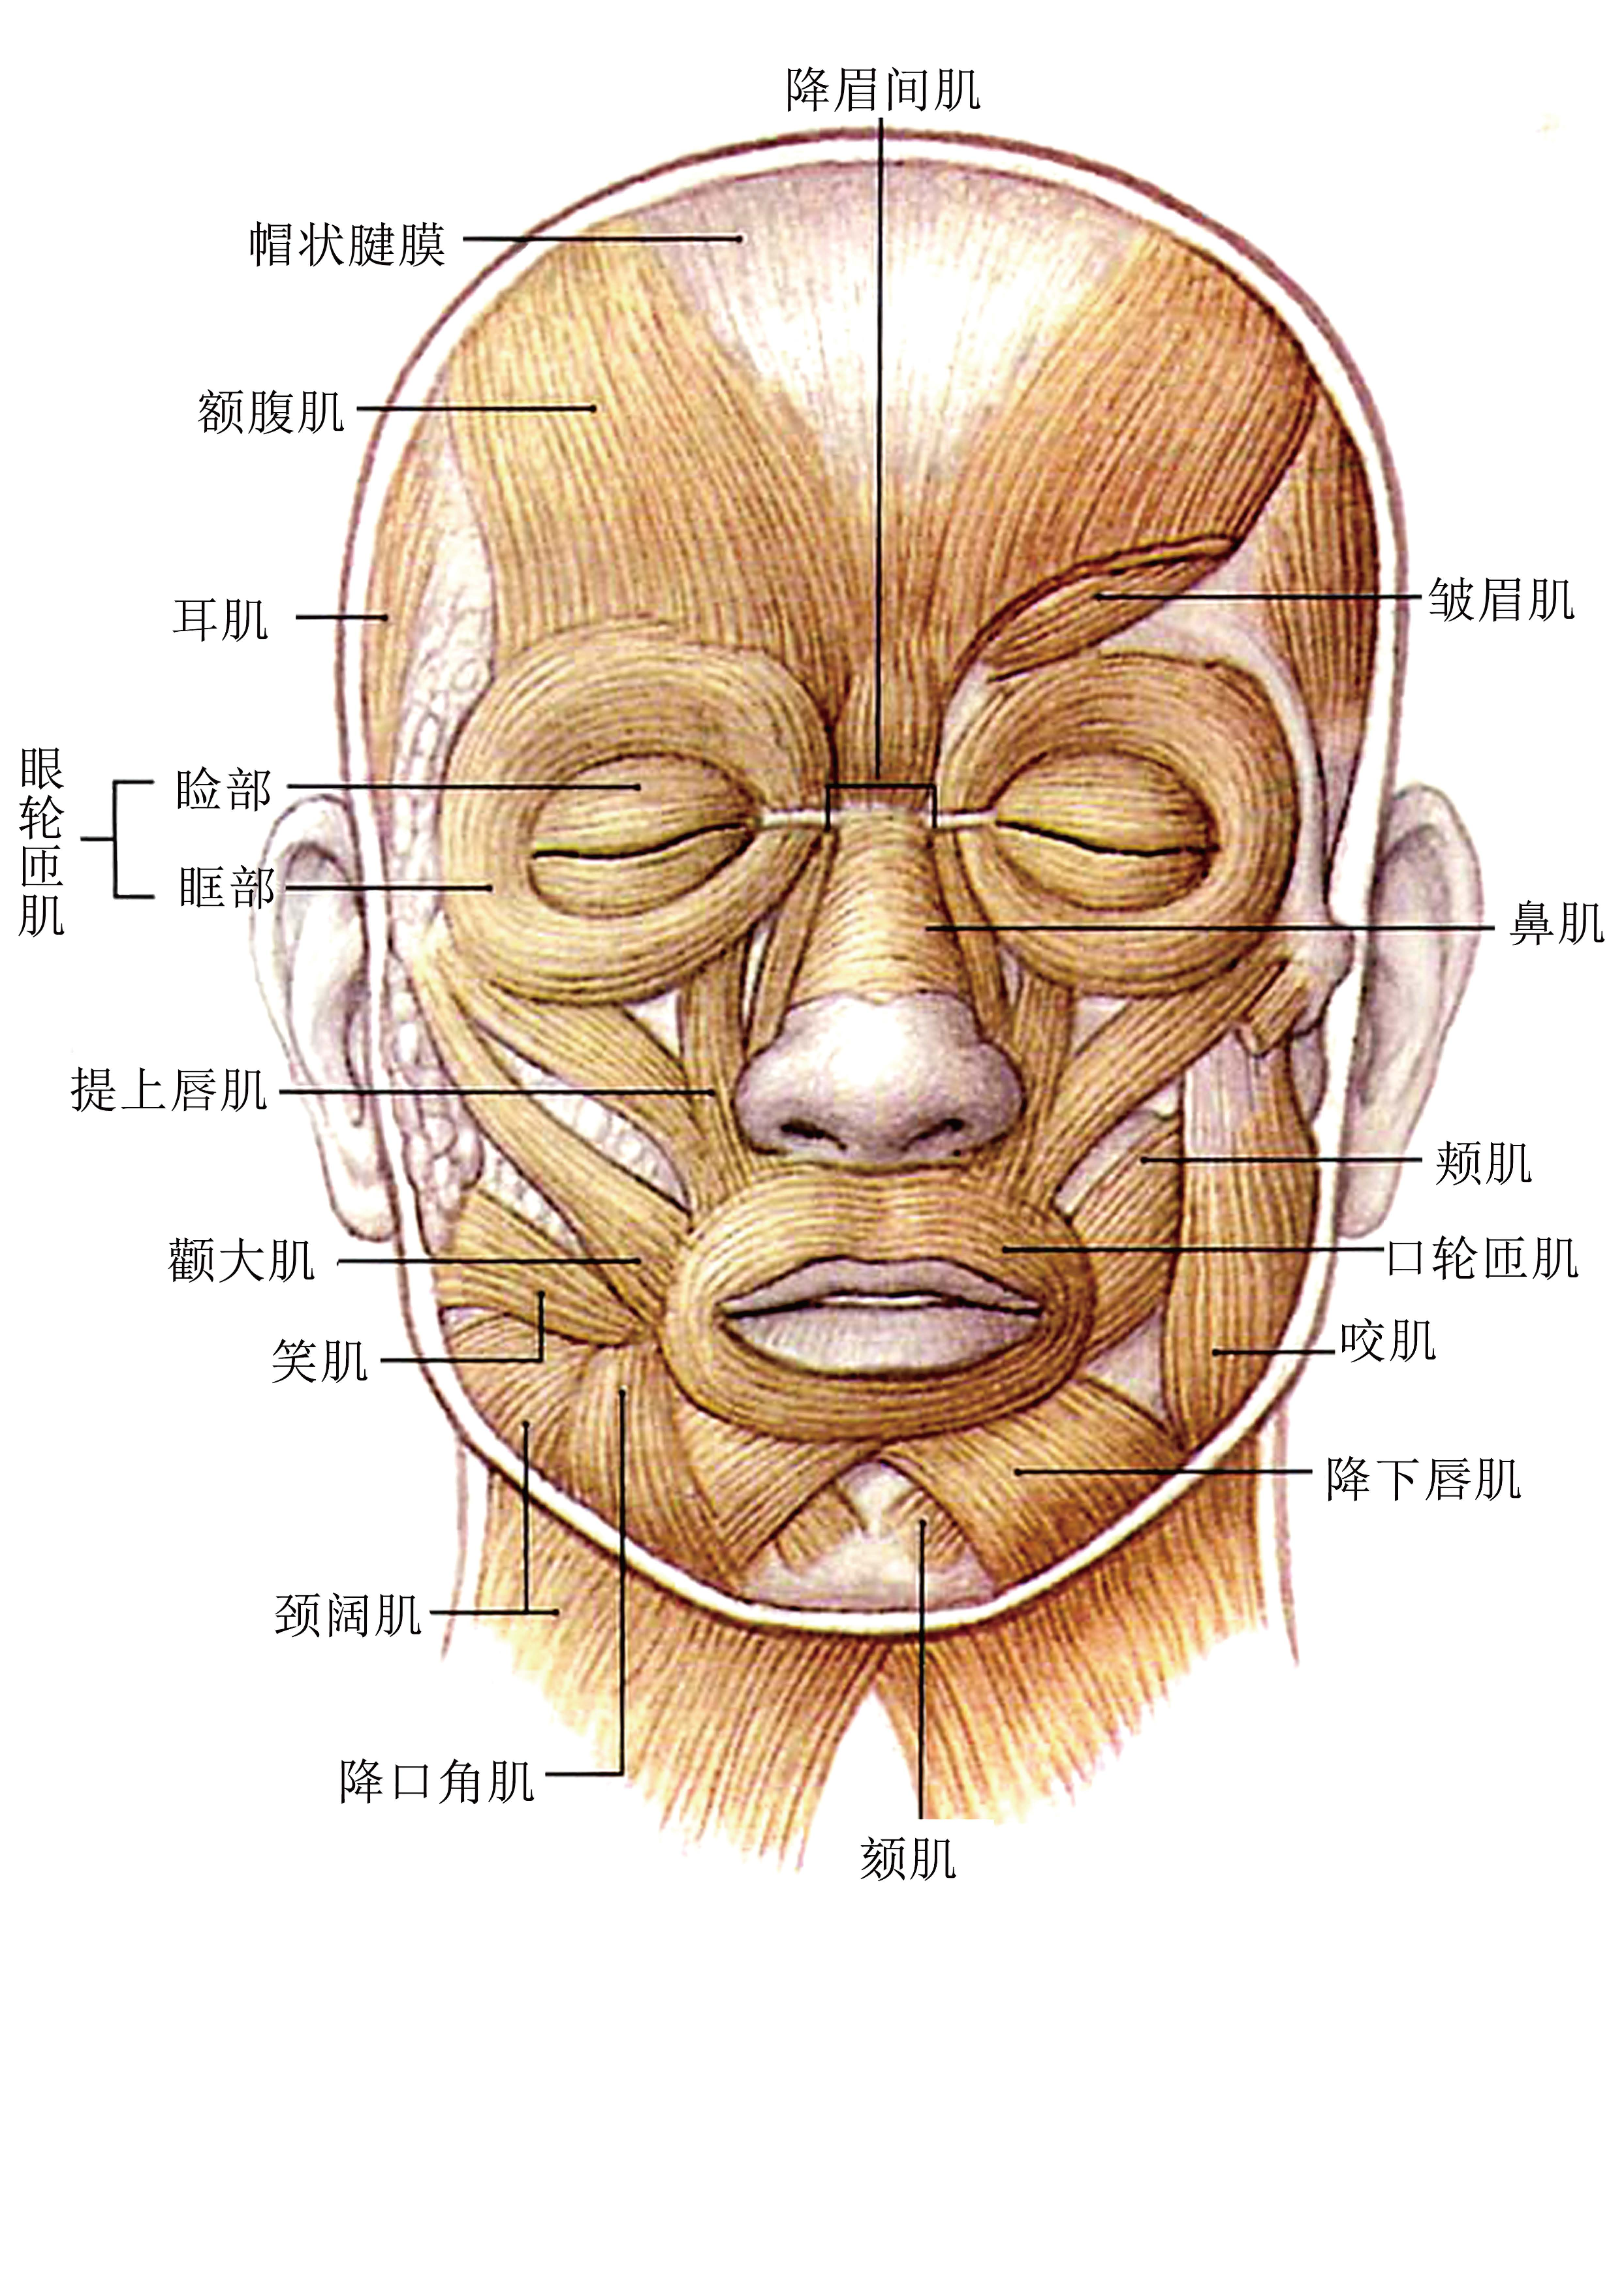
\includegraphics[width=0.28\textwidth]{ME2}
    \caption{人脸面部表情肌肉划分}
    \label{fig4}
\end{figure}

目前存在的宏表情和微表情数据集种类繁多且各具特色,但因为各类研究目的的差异,各类数据集间的迁移效果并不显著,存在着很大的局限性和个体差异性,存在的问题集中表现为以下几点:

首先,各个数据集建立标准不统一。对于常用的宏表情数据集,例如JAFFE和CK+两个宏表情数据集,他们在情感分类的标准上存在差异,JAFFE数据集将表情分为开心、愤怒、沮丧、讨厌、吃惊、恐惧和中性七类,而CK+数据集则在此基础上加入了轻蔑。同样与微表情数据集的分类方式也不一样,例如SMIC微表情数据集将表情分类为积极、消极和惊讶三类,CASME系列数据集将表情分类高兴、惊讶、悲伤、厌恶、恐惧、抑制和其他七种类型。另一方面,对于微表情数据集,不同的数据集之间诱发方式可能也存在差异,例如有的数据集使用自然诱发(SMIC、CASME),有的使用非自然状态下的模拟方式(USF-HD、Polikovsky)。此外差异性还表现在SMIC数据集没有对AU单元进行标注、CASME数据集的光照条件为。所以不同的数据库建立标准导致了难以使用统一的方法对数据集进行性能的评价。

其次,样本数量有限。目前各个数据集的样本数量较少,尤其是参与者的数量有限,这使得某些微表情现象不具有普遍意义,同时也难以提出较强的可说服性理论。



\section{微表情特征提取的一般方法}

\subsection{基于纹理信息的LBP-TOP特征提取符}

局部二值模式(Local Binary Pattern,LBP)是一种用来描述图像局部纹理特征的运算符,它具有旋转不变性和灰度不变性等显著的优点,在人脸识别方面被广泛应用\citep{Ojala2002Gray}。简单来说,就是对图像中的某一像素点的灰度值与其邻域的像素点的灰度值做比较,如果邻域像素值比该点大,则赋为1,反之,则赋为0。从图像的左上角开始,形成一个LBP编码,然后将该编码转换为一个十进制数。通过这种转换,可以将一个像素点与邻域的差值关系用一个数表示。

因为LBP特征记录的是像素点与邻域像素的差值关系,所以光照变化只会引起像素值的同增或同减,不会改变LBP值的大小,特别是在局部区域,所以LBP可以很好的保存图像中像素值的差值关系(如图~\ref{fig5}所示)。进一步的将LBP做直方图统计,这个直方图就可以用来作为纹理分析的特征算子。

\begin{figure}[!htbp]
    \centering
    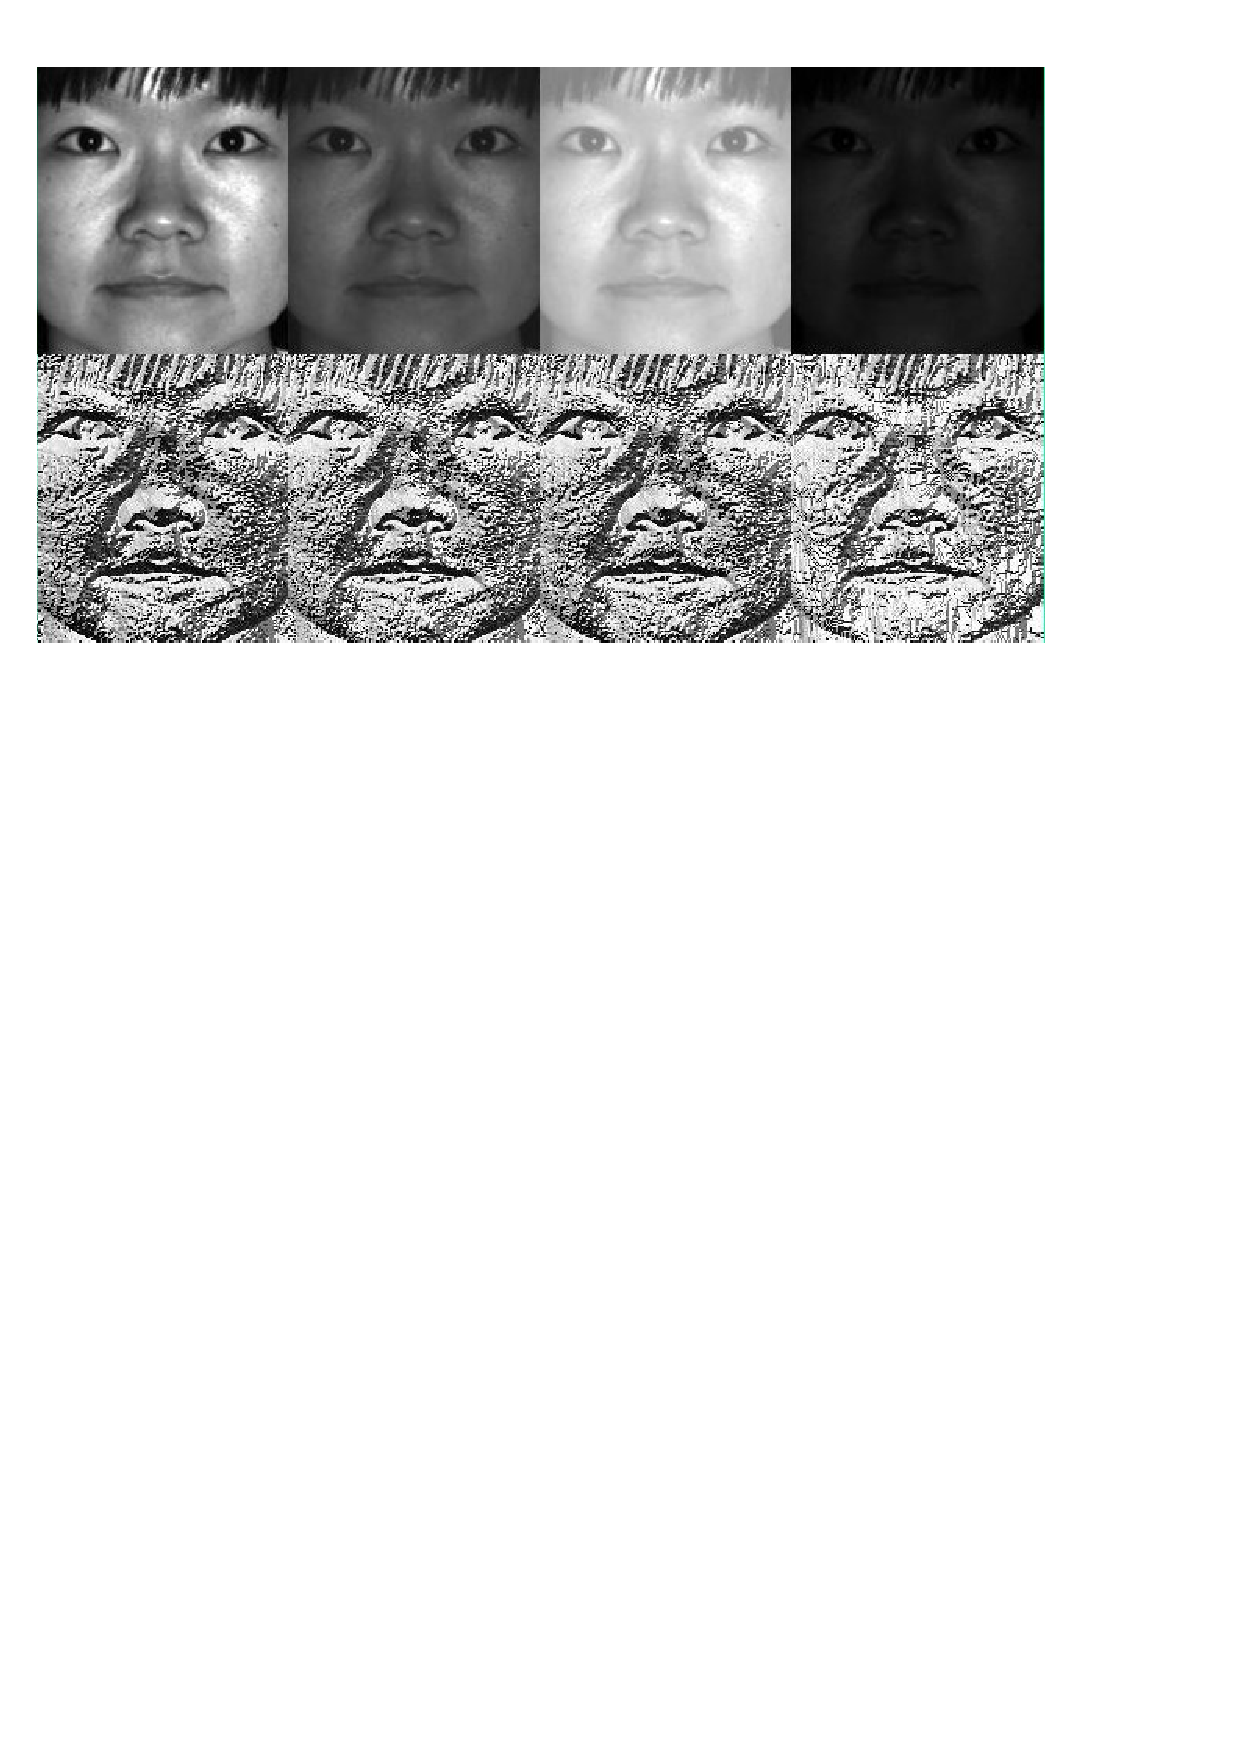
\includegraphics[width=0.5\textwidth]{LBP0}
    \caption{LBP特征的光照鲁棒性}
    \label{fig5}
\end{figure}

但是LBP只能处理单张的二维图像,对于视频或者图像序列则无能为力,2007年芬兰奥卢大学的Zhao等人提出了一种处理动态纹理的LBP特征提取符LBP-TOP,但是现在已经被广泛用于基于视频的人脸表情识别\citep{zhao2007dynamic}。

LBP-TOP是LBP从二维空间到三维空间的拓展,是在二维图像的X、Y方向上增加了一个沿着时间方向的T轴,形成了互相正交的XY、XT和YT三个平面。 以一个图像序列为单位组成一个立方体,对其划分合适的块参数(Blocksize),将一个小块作为一个小单元从三个不同的平面提取LBP特征生成该平面的特征直方图,将三个直方图级联为一个基于块的直方图,以同样的方式遍历整个图像序列立方体,生成最终的LBP-TOP特征直方图,如图~\ref{fig6}所示,$\textrm{LBP-TOP}^{1}$指一个小单元(图中的红色立方体)的LBP-TOP特征直方图,$\textrm{LBP-TOP}^{2}$指整个立方体的LBP-TOP特征直方图,关于Blocksize的划分将在章节\ref{chap:owner1}中讨论。

\begin{figure}[!htbp]
    \centering
    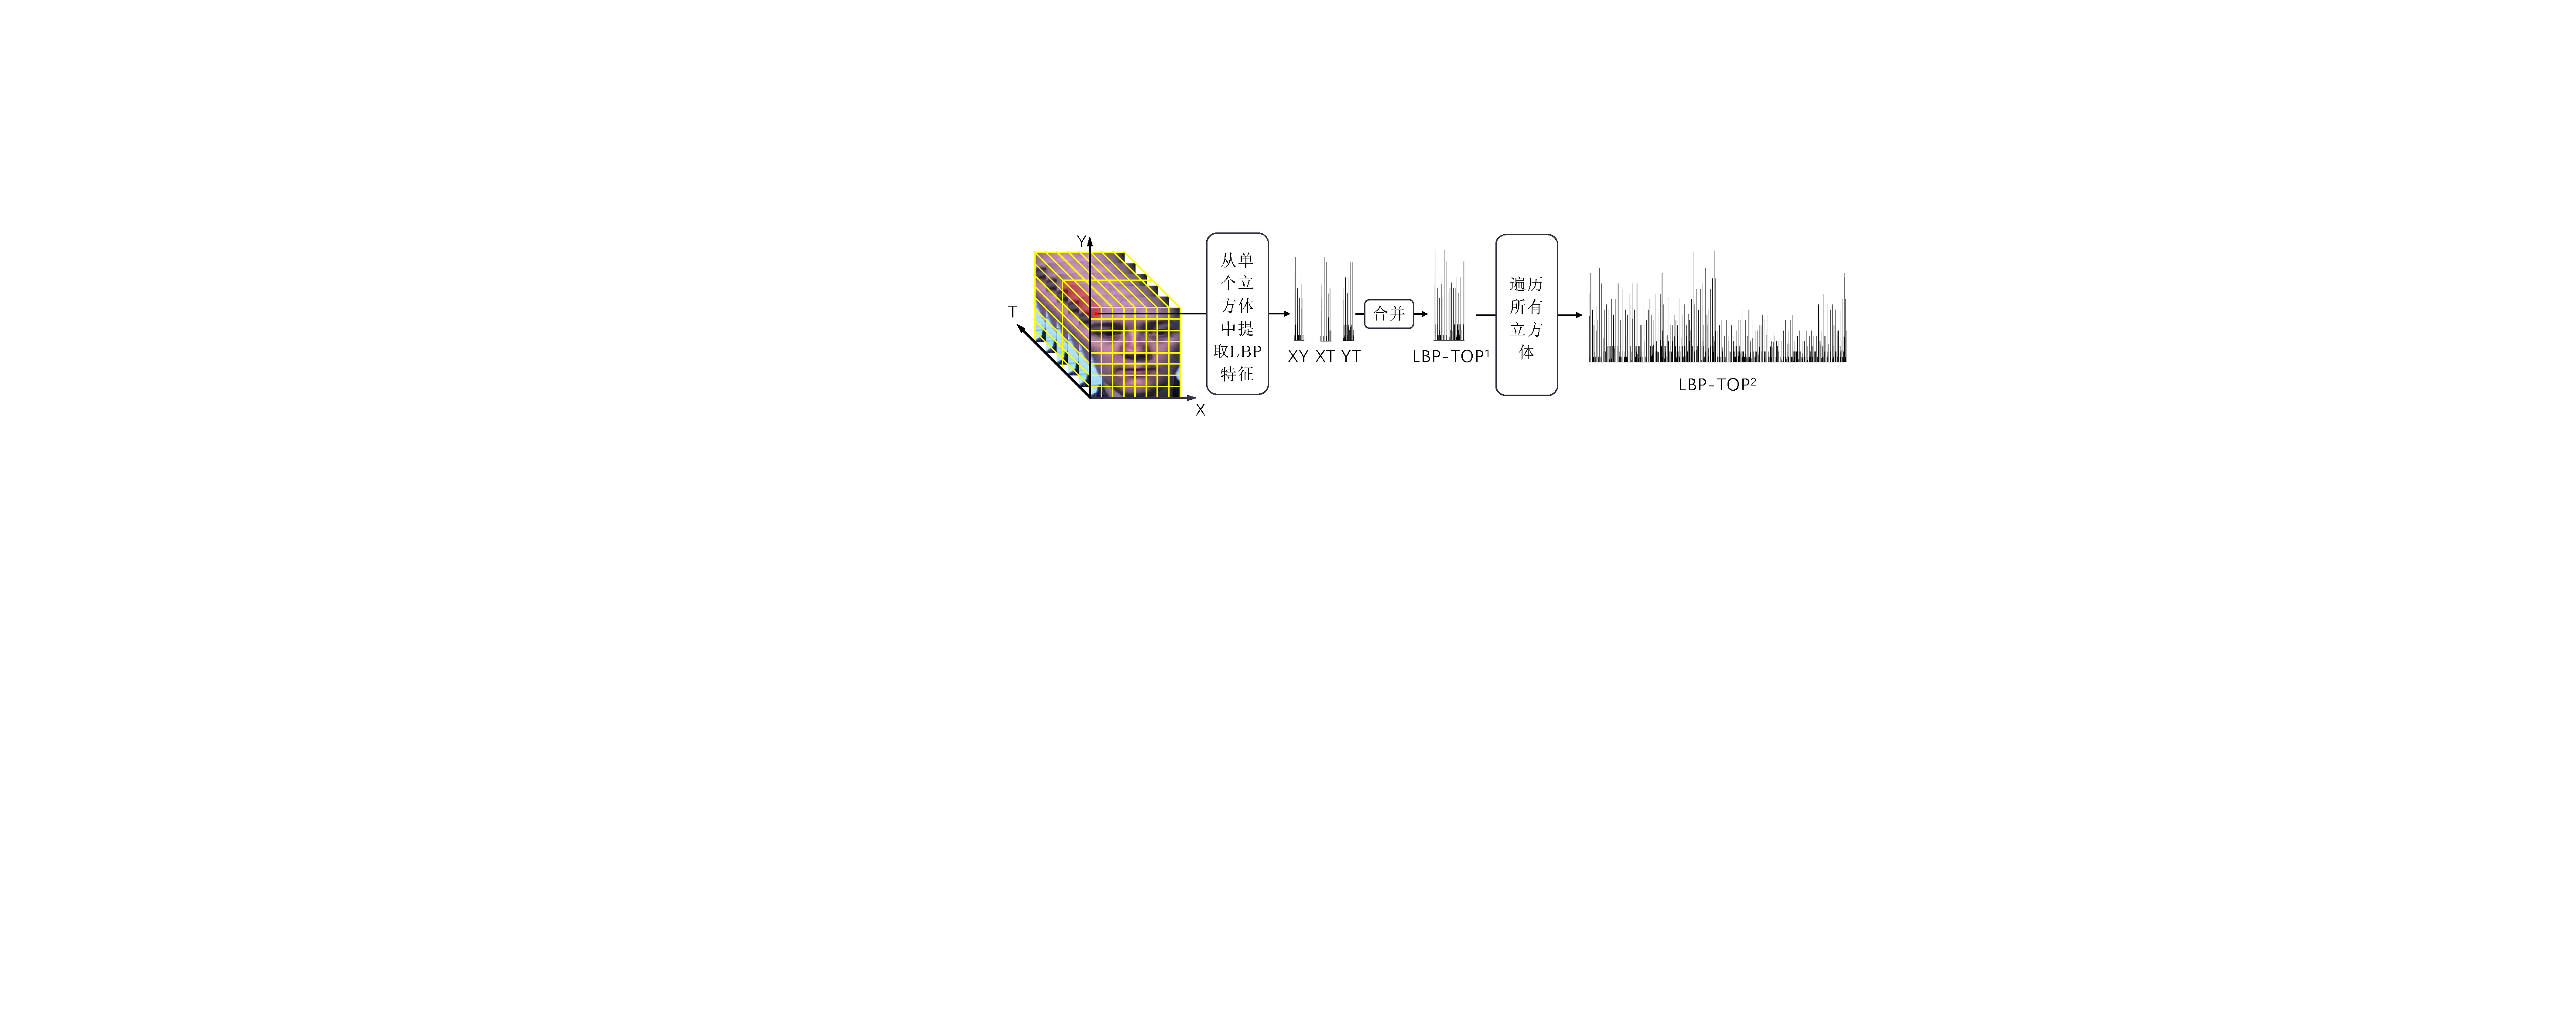
\includegraphics[width=0.9\textwidth]{LBP1}
    \caption{LBP-TOP特征提取过程}
    \label{fig6}
\end{figure}

\subsection{基于光流法的特征提取}

二十世纪五十年代心理学家Gibson在其著作\citepns{Gibson1950}中首次提出了环境光(Ambient optic)、环境光阵(Ambient optic array)、光流(Optic flow)和光流阵(Optic flow array)等基本概念。随后,一系列关于昆虫视觉机理方面的实验结果表明,大多数昆虫都可以通过光流测量自身的运动,进而通过积分获得自身飞行的距离。1976年,Poggio和Reichartdt等人在研究昆虫视觉时提出了关于光流的粗略计算形式\citep{poggio1976visual},1981年Horn和Lucas等人将二维速度场与灰度相联系,引入了光流约束方程,为光流计算做出了奠基性的工作\citep{Lucas1981, HORN1981185}。

光流是空间运动物体在观察成像平面上的像素运动的瞬时速度,是利用图像序列中像素在时间域上的变化以及相邻帧之间的相关性来找到上一帧跟当前帧之间存在的对应关系,从而计算出相邻帧之间物体的运动信息的一种方法。一般而言,光流是由于场景中前景目标本身的移动、相机的运动,或者两者的共同运动所产生的。Barron等人对多种光流计算技术进行了总结,按照理论基础与数学方法的区别把它们分成四种:(1)基于区域或者基于特征的匹配方法;(2)基于频域的方法;(3)基于梯度的方法;(4)基于能量的方法\citep{Barron1992}。光流的研究是利用图像序列中的像素强度数据的时域变化和相关性来确定各自像素位置的“运动”,即研究图像灰度在时间上的变化与景象中物体结构及其运动的关系,将二维图像平面特定坐标点上的灰度瞬时变化率定义为光流矢量。光流场(optical flow field)是运动场在二维图像平面上的投影(运动场,物体在三维真实世界中的运动),是一个二维矢量场,包含的信息是图像中像素点的灰度值发生变化趋势的瞬时速度矢量信息,那通俗的讲就是通过一个图像序列,把每张图像中每个像素的运动速度和运动方向找出来就是光流场。研究光流场的目的就是为了从图像序列中近似计算出不能直接得到的运动场。图~\ref{fig7}提供了光流场中光流的大小和方向的表现。

\begin{figure}[!htbp]
    \centering
    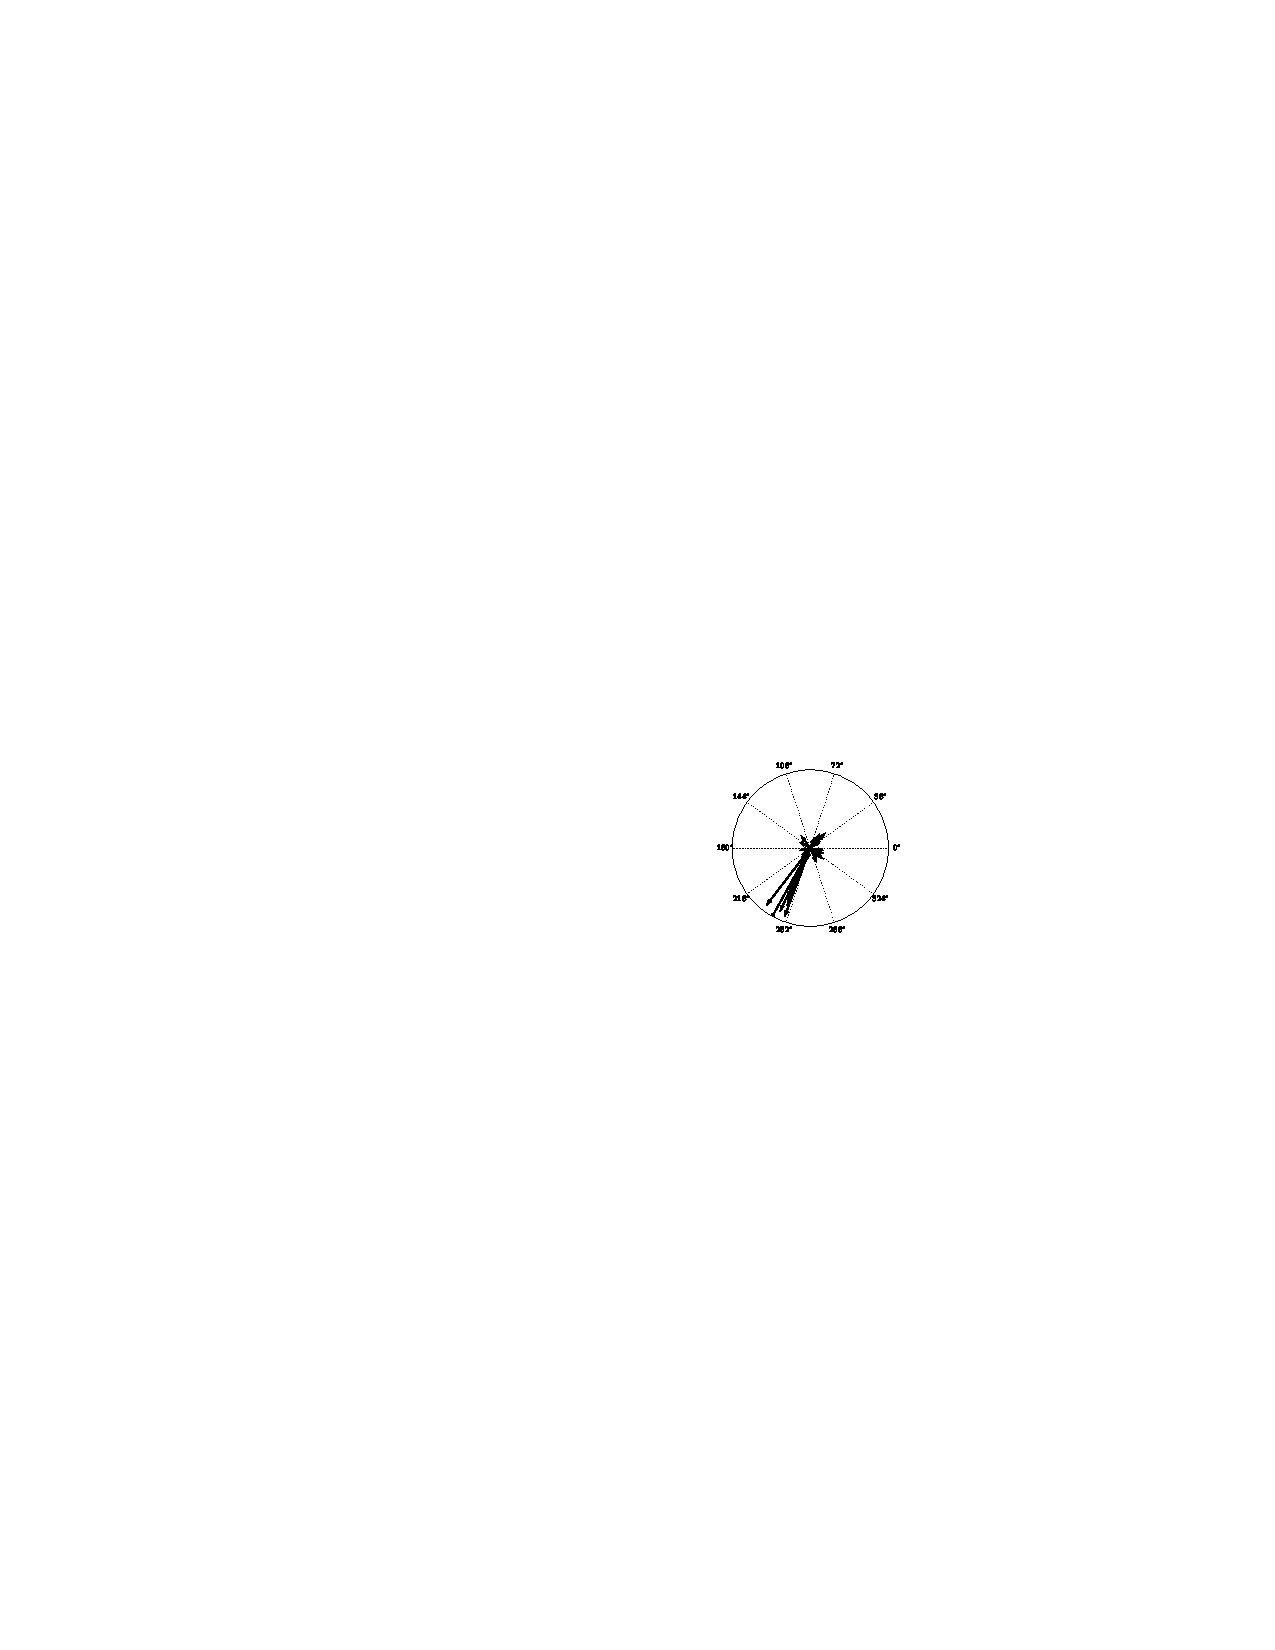
\includegraphics[width=0.30\textwidth]{OF0}
    \caption{光流大小和方向的表现}
    \label{fig7}
\end{figure}

光流法检测运动目标,其基本思想是赋予图像中的每一个像素点一个速度矢量,从而形成了该图像的运动场。图像上的点和三维物体上的点在某一特定的运动时刻是一一对应的,根据各像素点的速度矢量特征对图像进行动态的分析。若图像中不存在运动目标,那么光流矢量在整个图像区域则是连续变化的,而当物体和图像背景中存在相对运动时,运动物体所形成的速度矢量则必然不同于邻域背景的速度矢量,从而将运动物体的位置检测出来。但光流法的计算过于复杂,而且在实际情况中由于各种复杂的环境因素常常会导致计算结果出现很大的误差,故对它的使用必须是在建立一定前提假设的基础之上的:(1)相邻帧之间保持亮度恒定不变;(2)相邻帧的取帧时间保持连续或物体运动幅度小;(3)具有空间一致性,同一子图的像素点具有相同的运动。

光流不能由运动图像的局部信息来唯一的确定,例如,亮度等值线上的点或者亮度比较均匀的区域都无法唯一的确定其点的运动对应性,但是运动是可以进行观察得到。当人的眼睛观察运动物体时,物体的景象在人眼的视网膜上形成一系列连续变化的图像,这一系列连续变化的信息不断“流过”视网膜(即图像平面),由于它包含了目标运动的信息,因此可被观察者用来确定目标的运动情况。由此说明运动场和光流不一定是唯一对应的,即光流不一定是由物体运动产生的,反之如果物体发生了运动也不一定就能产生光流。但是一般情况下,表观运动和物体真实运动之间的差异是可以忽略的,可以用光流场代替运动场来分析图像中的运动目标及其相关的运动参数。

\subsection{基于Gabor的特征提取}

% Gabor特征是一种可以用来描述图像纹理信息的特征,Gabor滤波器的频率和方向与人类的视觉系统类似,特别适合于纹理表示与判别。Gabor特征主要依靠Gabor核在频率域上对信号进行加窗,从而能描述信号的局部频率信息。
% 说到Gabor核,不能不提到傅里叶变换。正是靠傅里叶变换,我们才能将信号转换到频率域,才能让Gabor核在频率域去加窗。而在原本的空间域中,一个Gabor核实际上就是一个高斯核与正弦波调制的结果,可以看做是高斯核应用在了正弦波的频域部分。
% 先对图像I(x,y)进行实数形式的Gabor变换,得到处理后的图像,直接提取特征的话,特征维数太高,不利于后续处理。一般对图像分块,然后计算每一块对应的能量。

Gabor小波与人类视觉系统中简单细胞的视觉刺激响应非常相似,它在提取目标的局部空间和频率域信息方面具有良好的特性\citep{Daugman1988,Kyrki2004Simple}。虽然Gabor小波本身并不能构成正交基,但在特定参数下可构成紧框架。Gabor小波对于图像的边缘敏感,能够提供良好的方向选择和尺度选择特性,而且对于光照变化不敏感,能够提供对光照变化良好的适应性。上述特点使Gabor小波被广泛应用于视觉信息理解。二维Gabor小波变换是在时频域进行信号分析处理的重要工具,其变换系数有着良好的视觉特性和生物学背景,因此被广泛应用于图像处理、模式识别等领域。与传统的傅立叶变换相比,Gabor小波变换具有良好的时频局部化特性。即非常容易地调整Gabor滤波器的方向、基频带宽及中心频率从而能够最好的兼顾信号在时空域和频域中的分辨能力;Gabor小波变换具有多分辨率特性即变焦能力。即采用多通道滤波技术,将一组具有不同时频域特性的Gabor小波应用于图像变换,每个通道都能够得到输入图像的某种局部特性,这样可以根据需要在不同粗细粒度上分析图像。此外,在特征提取方面,Gabor小波变换与其它方法相比:一方面其处理的数据量较少,能满足系统的实时性要求;另一方面,小波变换对光照变化不敏感,且能容忍一定程度的图像旋转和变形,当采用基于欧氏距离进行识别时,特征模式与待测特征不需要严格的对应,故能提高系统的鲁棒性。

无论从生物学的角度还是技术的角度,Gabor特征都有很大的优越性。研究表明,在基本视觉皮层里的简单细胞的感受野局限在很小的空域范围内,并且高度结构化。Gabor变换所采用的核与哺乳动物视觉皮层简单细胞2D感受野剖面非常相似,具有优良的空间局部性和方向选择性,能够抓住图像局部区域内多个方向的空间频率(尺度)和局部性结构特征。这样,Gabor分解可以看作一个对方向和尺度敏感的有方向性的显微镜。同时,二维Gabor函数也类似于增强边缘以及峰、谷、脊轮廓等底层图像特征,这相当于增强了被认为是面部关键部件的眼睛、鼻子、嘴巴等信息,同时也增强了诸于黑痣、酒窝、伤疤等局部特征,从而使得在保留总体人脸信息的同时增强局部特性成为可能.它的小波特性说明了Gabor滤波结果是描述图像局部灰度分布的有力工具,因此,可以使用Gabor滤波来抽取图像的纹理信息. 由于Gabor特征具有良好的空间局部性和方向选择性,而且对光照、姿态具有一定的鲁棒性,因此在人脸识别中获得了成功的应用。然而,大部分基于Gabor特征的人脸识别算法中,只应用了Gabor幅值信息,而没有应用相位信息,主要原因是Gabor相位信息随着空间位置呈周期性变化,而幅值的变化相对平滑而稳定,幅值反映了图像的能量谱,Gabor幅值特征通常称为Gabor能量特征(Gabor energy features)。Gabor小波可像放大镜一样放大灰度的变化,人脸的一些关键功能区域(眼睛、鼻子、嘴、眉毛等)的局部特征被强化,从而有利于区分不同的人脸图像。Gabor小波核函数具有与哺育动物大脑皮层简单细胞的二维反射区相同的特性,即具有较强的空间位置和方向选择性,并且能够捕捉对应于空间和频率的局部结构信息;Gabor滤波器对于图像的亮度和对比度变化以及人脸姿态变化具有较强的健壮性,并且它表达的是对人脸识别最为有用的局部特征。Gabor小波是对高级脊椎动物视觉皮层中的神经元的良好逼近,是时域和频域精确度的一种折中。

通过上面的分析,我们知道了,一个Gabor核能获取到图像某个频率邻域的响应情况,这个响应结果可以看做是图像的一个特征。那么,我们如果用多个不同频率的Gabor核去获取图像在不同频率邻域的响应情况,最后就能形成图像在各个频率段的特征,这个特征就可以描述图像的频率信息了,由于纹理特征通常和频率相关,因此Gabor核经常用来作为纹理特征。

\section{相关深度学习网络}

深度学习方法作为机器学习尤其是神经网络方法的一种,在图像处理、视频分析和语音识别等领域产生了许多成功的案例。端到端的神经网络模型能够通过学习大量高维数据进行分类和预测,这减少了人工特征工程的繁杂操作。卷积神经网络作为应用最广泛的深度学习方法之一,目前在很多图像相关领域都处于无可替代的地位。卷积神经网络最早出现在论文\citepns{lecun1998gradient}的研究中,在过去的几年里,卷积神经网络经过了大量的分层、分块等设计的修改,诞生了许多成功的衍生网络如AlexNet\citep{krizhevsky2012imagenet}、VGG-Net\citep{Simonyan2014Very}和GoogLeNet\citep{szegedy2015going}等。最近,有很多将深度学习应用于微表情识别的研究,然而,由于是在小数据集上使用的深度网络,所获得的识别准确度仅在随机水平左右。

\subsection{三维卷积神经网络}

二维卷积神经网络被认为是解决图像识别问题的一种强大的模型,但将二维卷积神经网络应用到视频中却并非易事,在视频中应用二维卷积神经网络一个简单的方法就是对每一帧运用卷积来识别,但是这种方法并没有考虑到连续帧间的时间维度信息。一些研究表明,三维卷积能够从空间和时间两个维度提取特征,从而获取多个相邻帧中编码的运动信息。三维卷积神经网络从输入帧中生成多个通道的信息,并结合所有通道的信息得到最终的特征表示。该方法应用到现实环境中的人类行为识别中,在不依赖于人工提取的特性的情况下取得了优异的性能\citep{Shuiwang20133D}。

三维卷积是通过将一个三维核与叠加在一起的多个连续帧形成的立方体进行卷积来实现的。在这个结构中,卷积层中每一个特征映射都会与前一层中多个相邻的连续帧相连,从而获取运动信息。需要注意的是:三维卷积核只能从立方体中提取一类特征,因为在整个立方体中卷积核的权值都是一样的,也就是共享权值。所以我们可以采用多种卷积核,以提取多种特征。对于卷积神经网络有一个通用的设计规则,在后面的层(离输出层近的)特征映射的个数应该增加,这样就可以从低级的特征映射组合产生更多类型的特征。

\begin{figure}[!htbp]
    \centering
    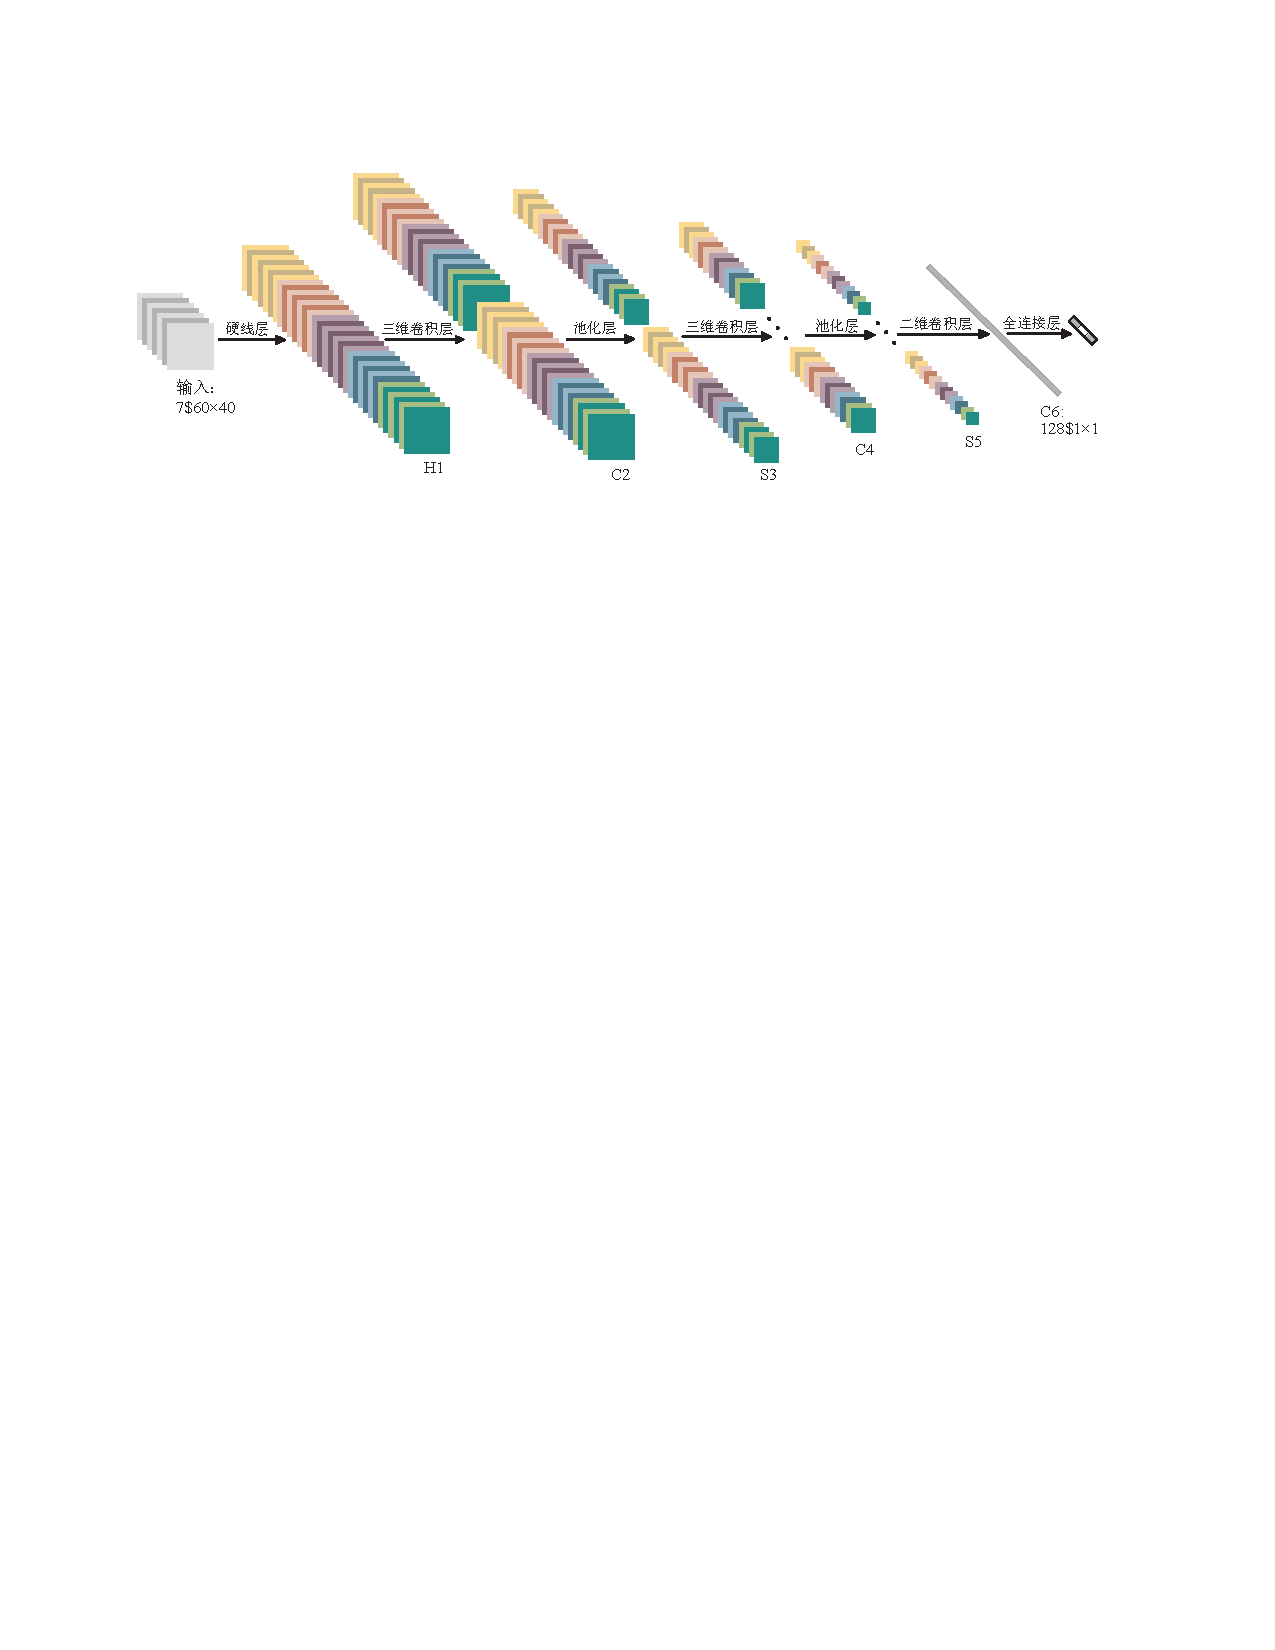
\includegraphics[width=0.95\textwidth]{3DCNN1}
    \caption{三维卷积神经网络架构}
    \label{fig8}
\end{figure}

如图~\ref{fig8}所示,该架构包含一个硬线层、三个卷积层、两个池化层和一个全连接层。每个三维卷积核卷积的立方体是连续的七帧,每帧块大小为$60\times40$;第一层应用了一个固定的硬线核去对原始的帧进行处理,产生多个通道的信息,然后对多个通道分别处理。最后再将所有通道的信息组合起来得到最终的特征描述。

H1为硬线层(Hardwired),每帧提取五个通道的信息,分别是灰度、$x$和$y$方向的梯度,$x$和$y$方向的光流。其中,前面三个都可以每帧都计算。然后水平和垂直方向的光流场需要两个连续帧才确定。

C2为卷积层(Convolution),以硬线层的输出作为该层的输入,用一个三维卷积核在五个通道的每一个通道分别进行卷积。同时为了增加特征映射的个数(实际上就是提取不同的特征),在每一个位置都采用两个不同的卷积核。

S3为池化层(Sub-sampling),得到相同数目但是空间分辨率降低的特征映射。

C4为卷积层,对五个通道分别采用三维卷积核,同样,为了增加特征映射个数,在每个位置都采用三种不同的卷积核。

S5为池化层,对每个特征映射采用核进行降采样操作,在这个阶段,每个通道的特征映射都很小。

C6为卷积层,此时对每个特征映射采用二维卷积核进行卷积操作,然后输出为减小到$1×1$大小的特征映射。

经过多层的卷积和下采样后,每连续7帧的输入图像都被转化为一个128维的特征向量,这个特征向量捕捉了输入帧的运动信息。输出层的节点数与行为的类型数目一致,而且每个节点与C6中这128个节点是全连接的。最后,采用一个线性分类器来对这128维的特征向量进行分类,实现行为的识别。

\subsection{残差神经网络}

增加网络的宽度和深度可以很好的提高网络的性能,深的网络一般都比浅的的网络效果好,但对于原来的网络,如果简单地增加深度,会导致梯度弥散或梯度爆炸。对于该问题的解决方法是正则化初始化和中间的正则化层(Batch Normalization),这样的话可以训练几十层的网络。虽然通过上述方法能够训练,但是又会出现退化问题。在实验中的表现就是虽然网络层数增加,但在训练集上的准确率却饱和甚至下降了(这个不能简单的解释为过拟合现象,因为过拟合时应该在训练集上表现的更好)。通过浅层网络等同映射构造深层模型,结果深层模型并没有比浅层网络有等同或更低的错误率,推断退化问题可能是因为深层的网络并不是那么好训练,也就是求解器很难去利用多层网络拟合同等函数。

针对这个问题He等在2015年提出了一种全新的网络,叫深度残差神经网络(Deep residual neural network),它允许网络尽可能的加深,其中引入了全新的结构,如图~\ref{fig9}所示\citep{he2016deep}。

\begin{figure}[!htbp]
    \centering
    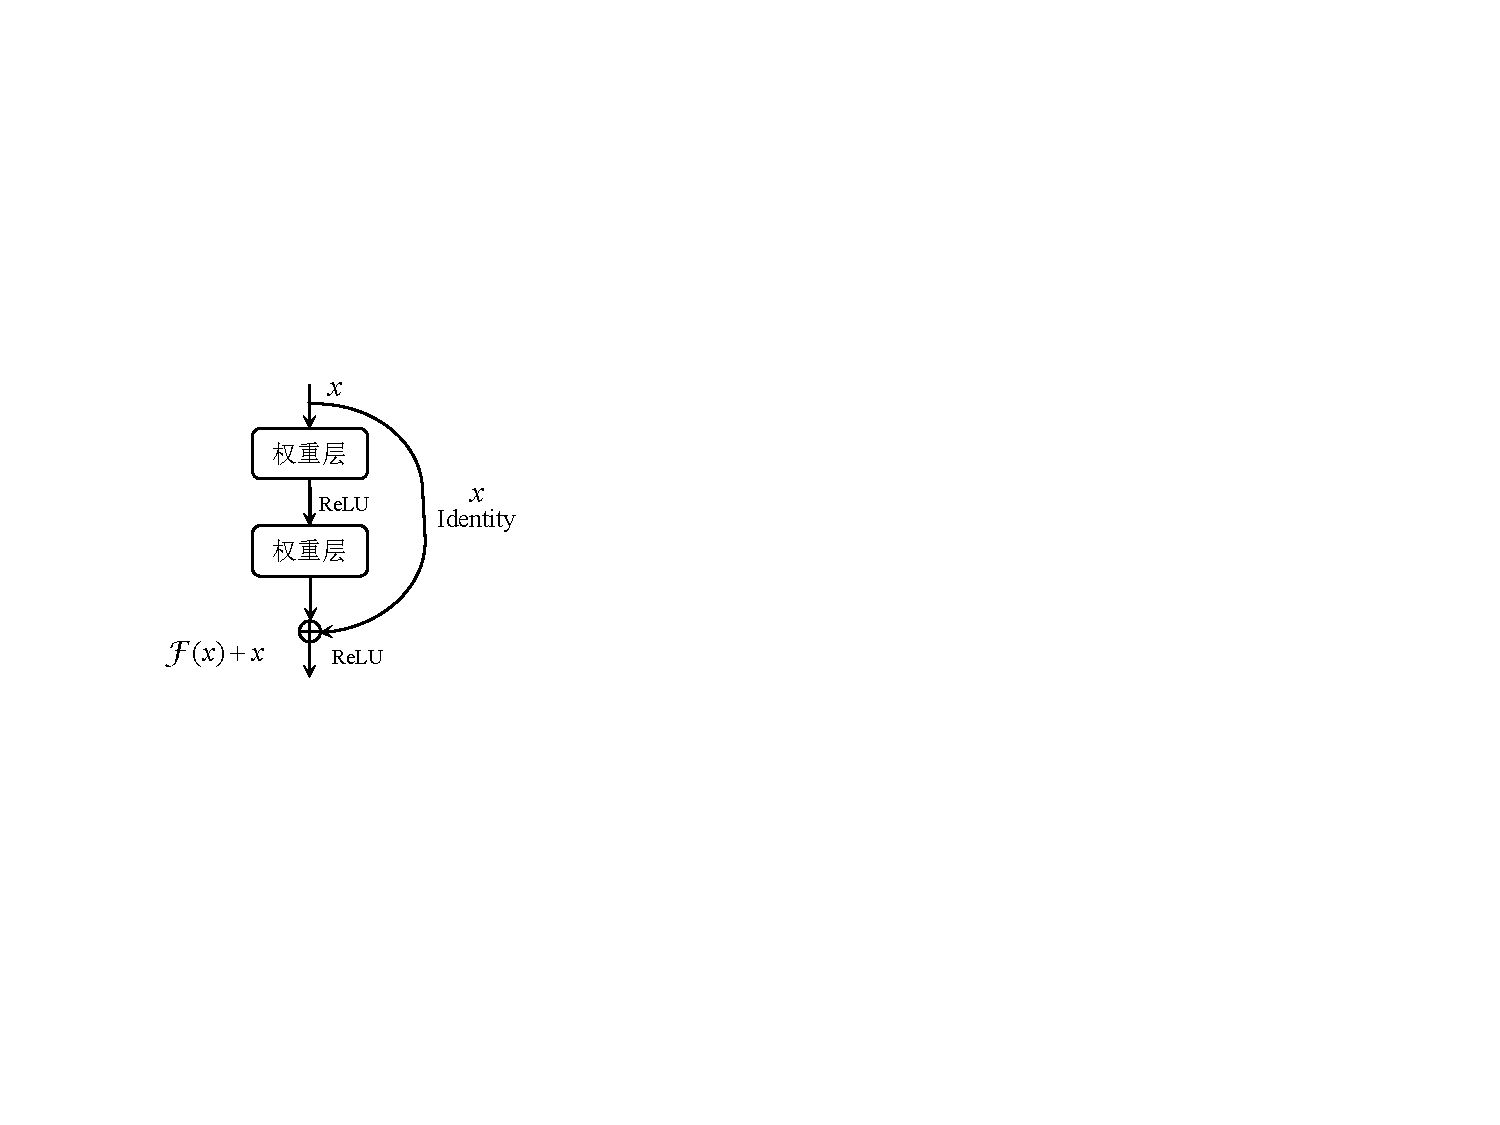
\includegraphics[width=0.40\textwidth]{RESNET0}
    \caption{ResNet的残差学习模块}
    \label{fig9}
\end{figure}

理论上,对于“随着网络加深,准确率下降”的问题,ResNet提出了两种Mapping:一种是Identity mapping,指图~\ref{fig9}中的弧线,另一种是Residual mapping,指除了弧线以外的部分,所以最后的输出是$y=\mathcal{F}\left ( x \right )+x$ 。Identity mapping指自身,也就是公式中的$x$ ,而Residual mapping指的是“差”,也就是$y-x$ ,所以残差指的就是$\mathcal{F}\left (x \right )$部分。如果网络已经到达最优,继续加深网络,Residual mapping将被转化为0,只剩下Iidentity mapping,这样理论上网络一直处于最优状态了,网络的性能也就不会随着深度增加而降低了。

由上可以看出残差网络t的主要思想是在网络中增加了直连通道,即Highway network的思想,它允许原始输入信息直接传到后面的层中\citep{Srivastava2015Highway},这样的话这一层的神经网络可以不用学习整个的输出,而是学习上一个网络输出的残差。

% 残差网络以前在不增加网络复杂性的情况下,在基于图像的识别任务上实现了最优性能。残差网络通常使用残差块来构建网络,而典型的残差块如图~\ref{fig9}所示。在残差块中,将添加一个捷径来执行标识映射(通过元素汇总实现),这有助于减少退化问题。捷径还加快了训练过程,几乎不引入额外的参数和计算。

传统的卷积网络或者全连接网络在信息传递的时候或多或少会存在信息丢失、损耗等问题,同时还会导致梯度弥散或梯度爆炸,导致很深的网络无法训练。残差网络在一定程度上解决了这个问题,通过直接将输入信息绕道传到输出,保护信息的完整性,整个网络只需要学习输入、输出差别的那一部分,简化学习目标和难度。残差网络的结构可以极快的加速神经网络的训练,模型的准确率也有比较大的提升。残差网络在ImageNet比赛Classification任务上获得第一名,因为它“简单与实用”并存,之后很多方法都建立在ResNet50或者ResNet101的基础上完成,检测、分割、识别等领域都纷纷使用残差网络,Alpha zero也使用了残差网络,所以可见残差网络确实很好用。

\chapter{基于传统机器学习方法的低分辨率环境下微表情识别}\label{chap:owner1}

微表情属于常规性非言语行为,可以真实的表达人类隐藏的情感。它在国家安全、计算机辅助医疗等领域有着非常广泛的应用,这鼓励我们开展微表情自动识别的研究。然而,从监控视频中获取的图像容易出现质量低下等问题,给实际应用带来非常大的困难,使得所有研究都只能在实验层面。由于通过监控视频所捕获图像的质量较低,现有的算法无法达到预期的效果。针对这一问题,我们对低分辨率情况下模糊人脸的微表情识别问题进行了全面的研究并提出了完整的低分辨率环境下微表情识别框架。实验结果表明,该框架在低分辨率情况下的微表情识别中取得了优异的成果。

目前常规的微表情识别算法虽然取得了良好的识别效果,但其性能在很大程度上取决于人脸视频片段的质量。一旦用于识别的人脸视频片段质量较差(如分辨率较低),章节\ref{chap:relate}中提及的算法就无法正常工作。原因主要在两个方面:(1)低分辨率图像丢失了大量的纹理信息,导致从低分辨率图像序列中提取可用特征变的困难\citep{lei2011local}。(2)低分辨率图像与高分辨率图像质量(不同分辨率、不同清晰度)不一致,导致我们在测试阶段无法直接使用低分辨率图像作为输入。同时,当处于真实环境时,从监控录像中获取的人脸图像通常只占整个画面的一小部分,例如,用于微表情识别的SMIC数据集的人脸分辨率为$190\times230$(SMIC数据集的分辨率为$640\times480$)。然而更严重的是,常规监控视频捕捉到的图像序列的人脸分辨率往往在$50\times50$(或更低)以下。这意味着之前的微表情识别方法不能直接用于处理低分辨率的情况。因此,对低分辨率环境下的微表情识别的研究具有重要意义和挑战性。

\begin{figure}[!htbp]
    \centering
    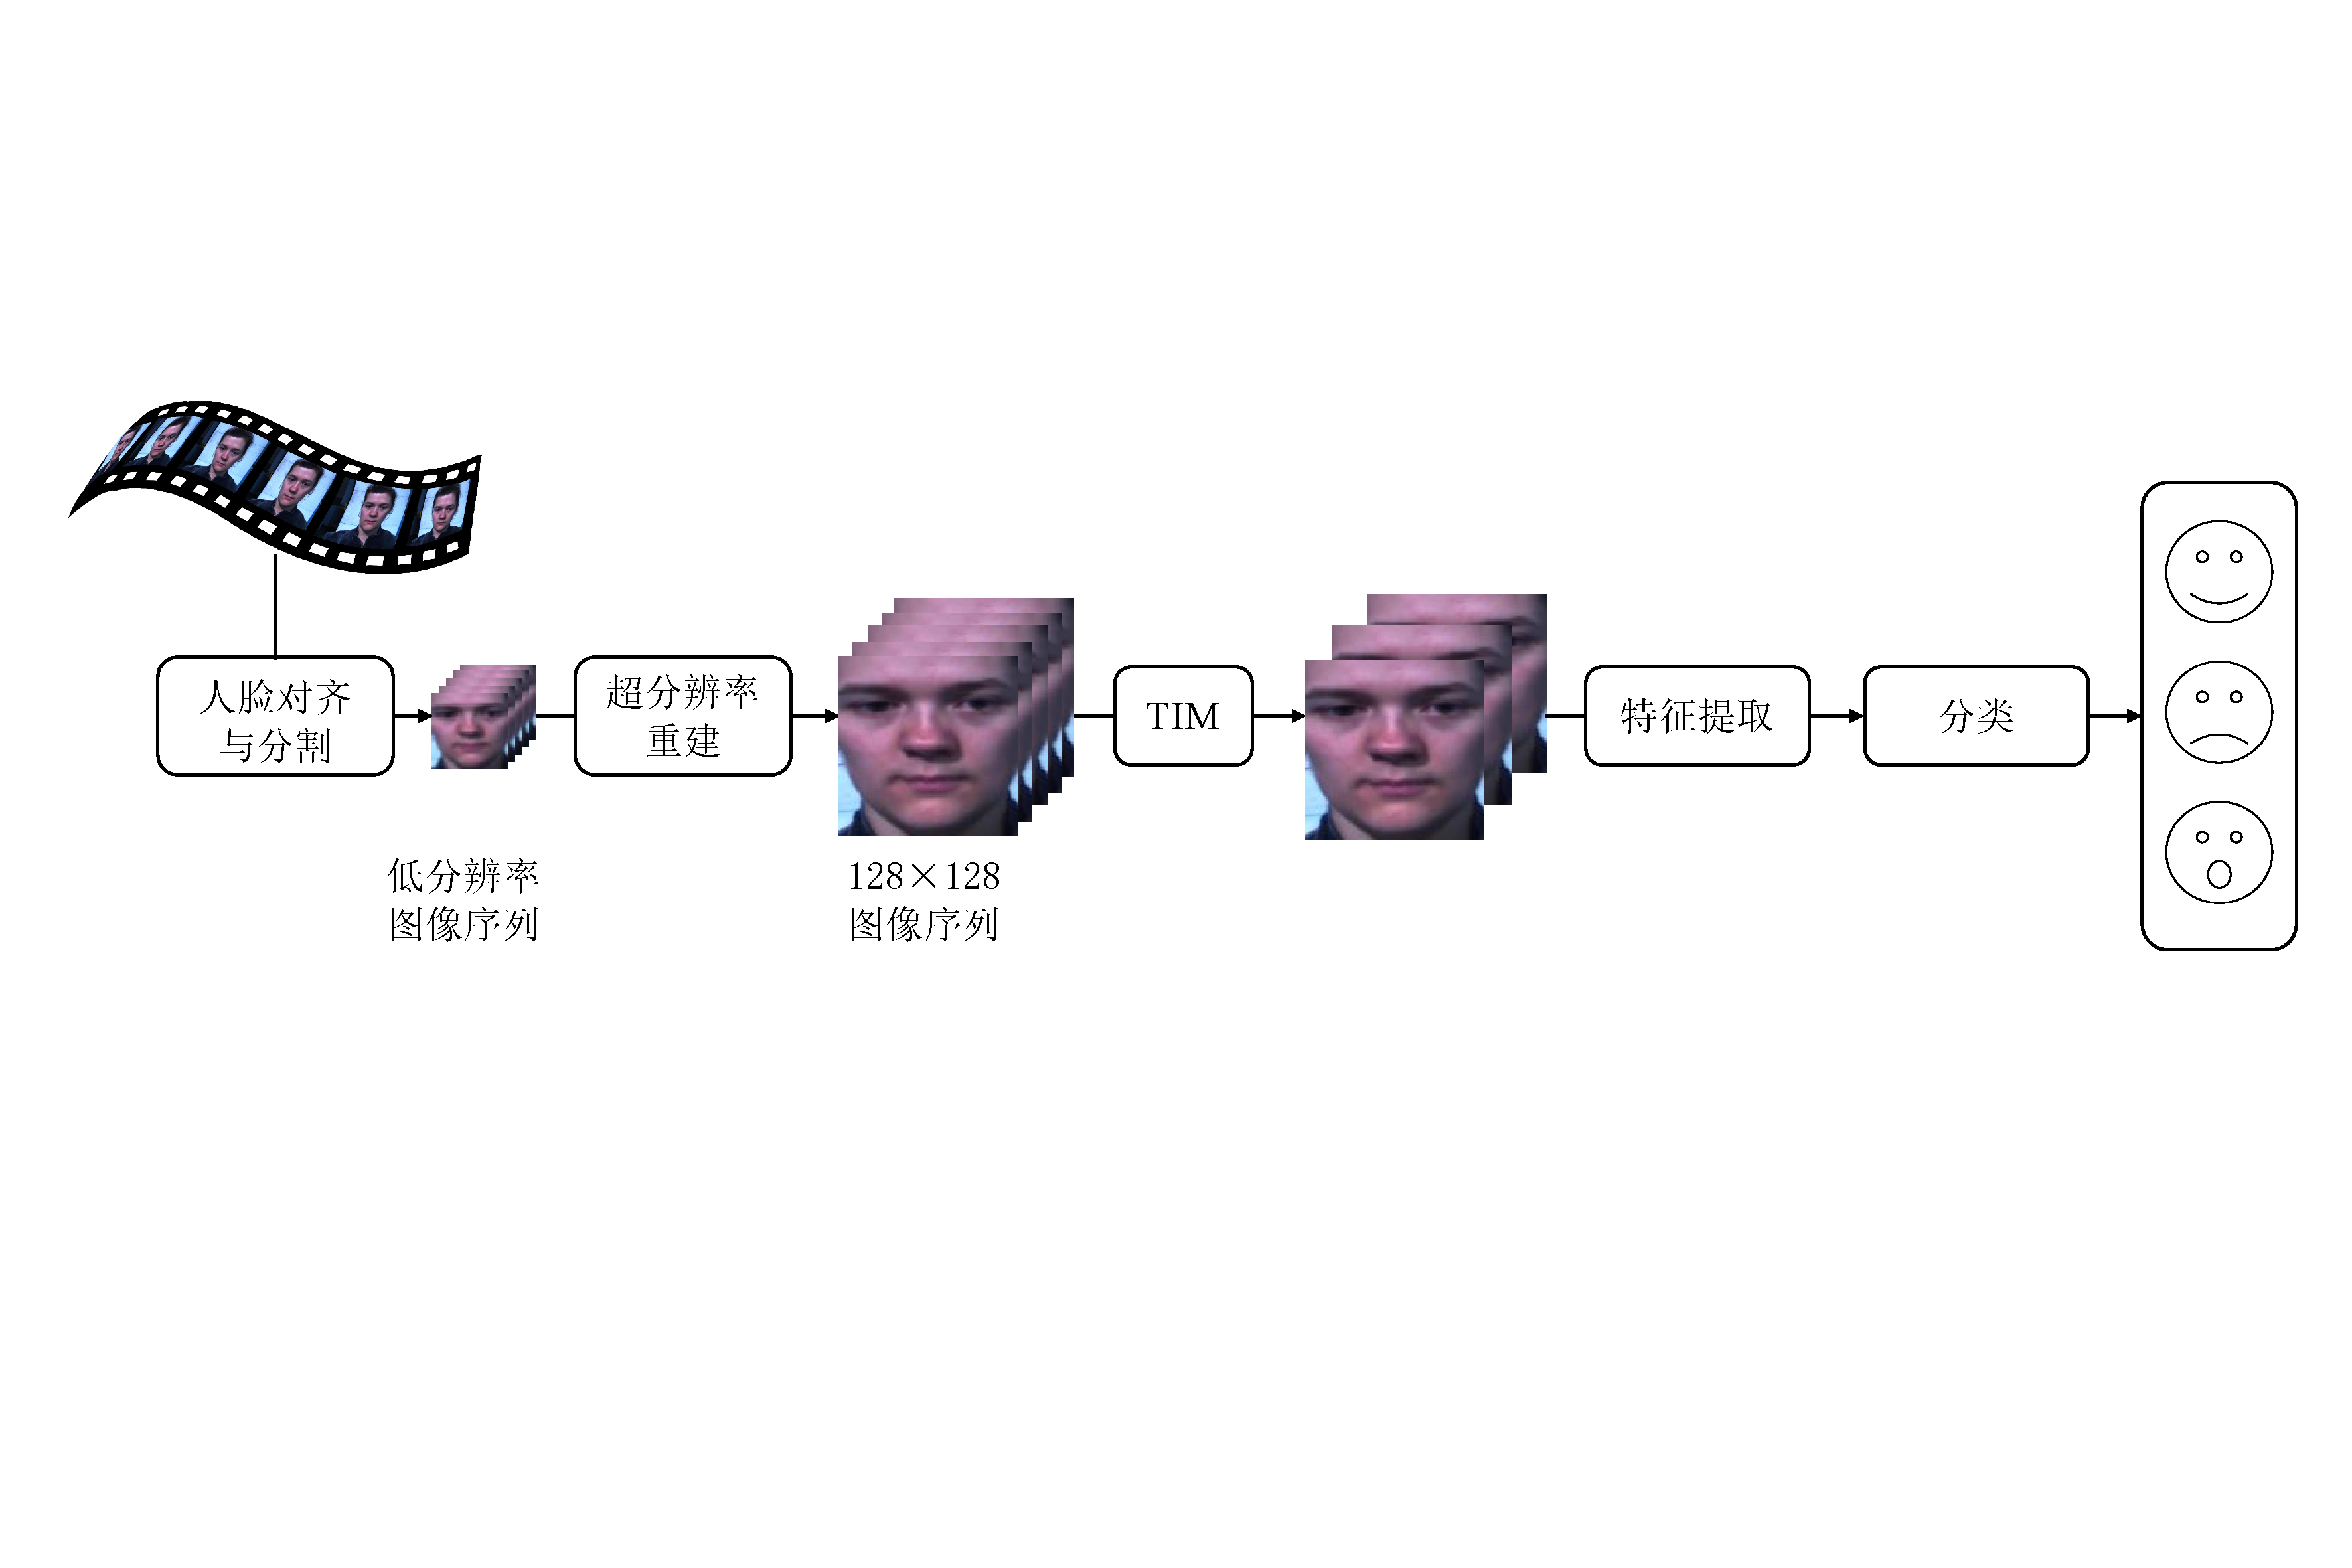
\includegraphics[width=0.98\textwidth]{LR0}
    \caption{低分辨率环境下微表情识别框架}
    \label{fig10}
\end{figure}

为了解决上述问题,我们利用最新的人脸Hallucination方法进行了低分辨率微表情识别的研究。我们首先对低质量的人脸图像序列Hallucination处理,以近似的重建出丢失的动态特征。然后,我们再采用传统的微表情识别算法识别低质量的微表情图像序列。我们评估了不同分辨率下微表情识别的准确率,研究了分辨率与识别准确率之间的关系。总的来说,本章的目的是全面研究分辨率对微表情识别的影响,同时提出一个基于传统机器学习方法的处理低质量条件下微表情识别任务的框架。

如图~\ref{fig10}所示,低分辨率微表情识别过程包括图像序列预处理、超分辨率重建、特征提取和分类。详细内容将在本章的以下部分展开描述:

\section{低分辨率微表情数据获取}

目前常用的微表情识别的数据集有很多,如SMIC和CASME等。然而,这些数据集都是专业相机在严苛环境下获取的高清图像序列,表~\ref{tab3}详细描述了各数据集的参数。图~\ref{fig11}列举了SMIC-HS数据集中一个视频片段中的两帧。我们可以在红色框的范围中发现面部表情的细微变化,特别是白色椭圆区域和白色箭头指向的位置运动更为明显。然而,如果图像质量过低,这些细节很难被注意到。

\begin{figure}[!htbp]
\centering
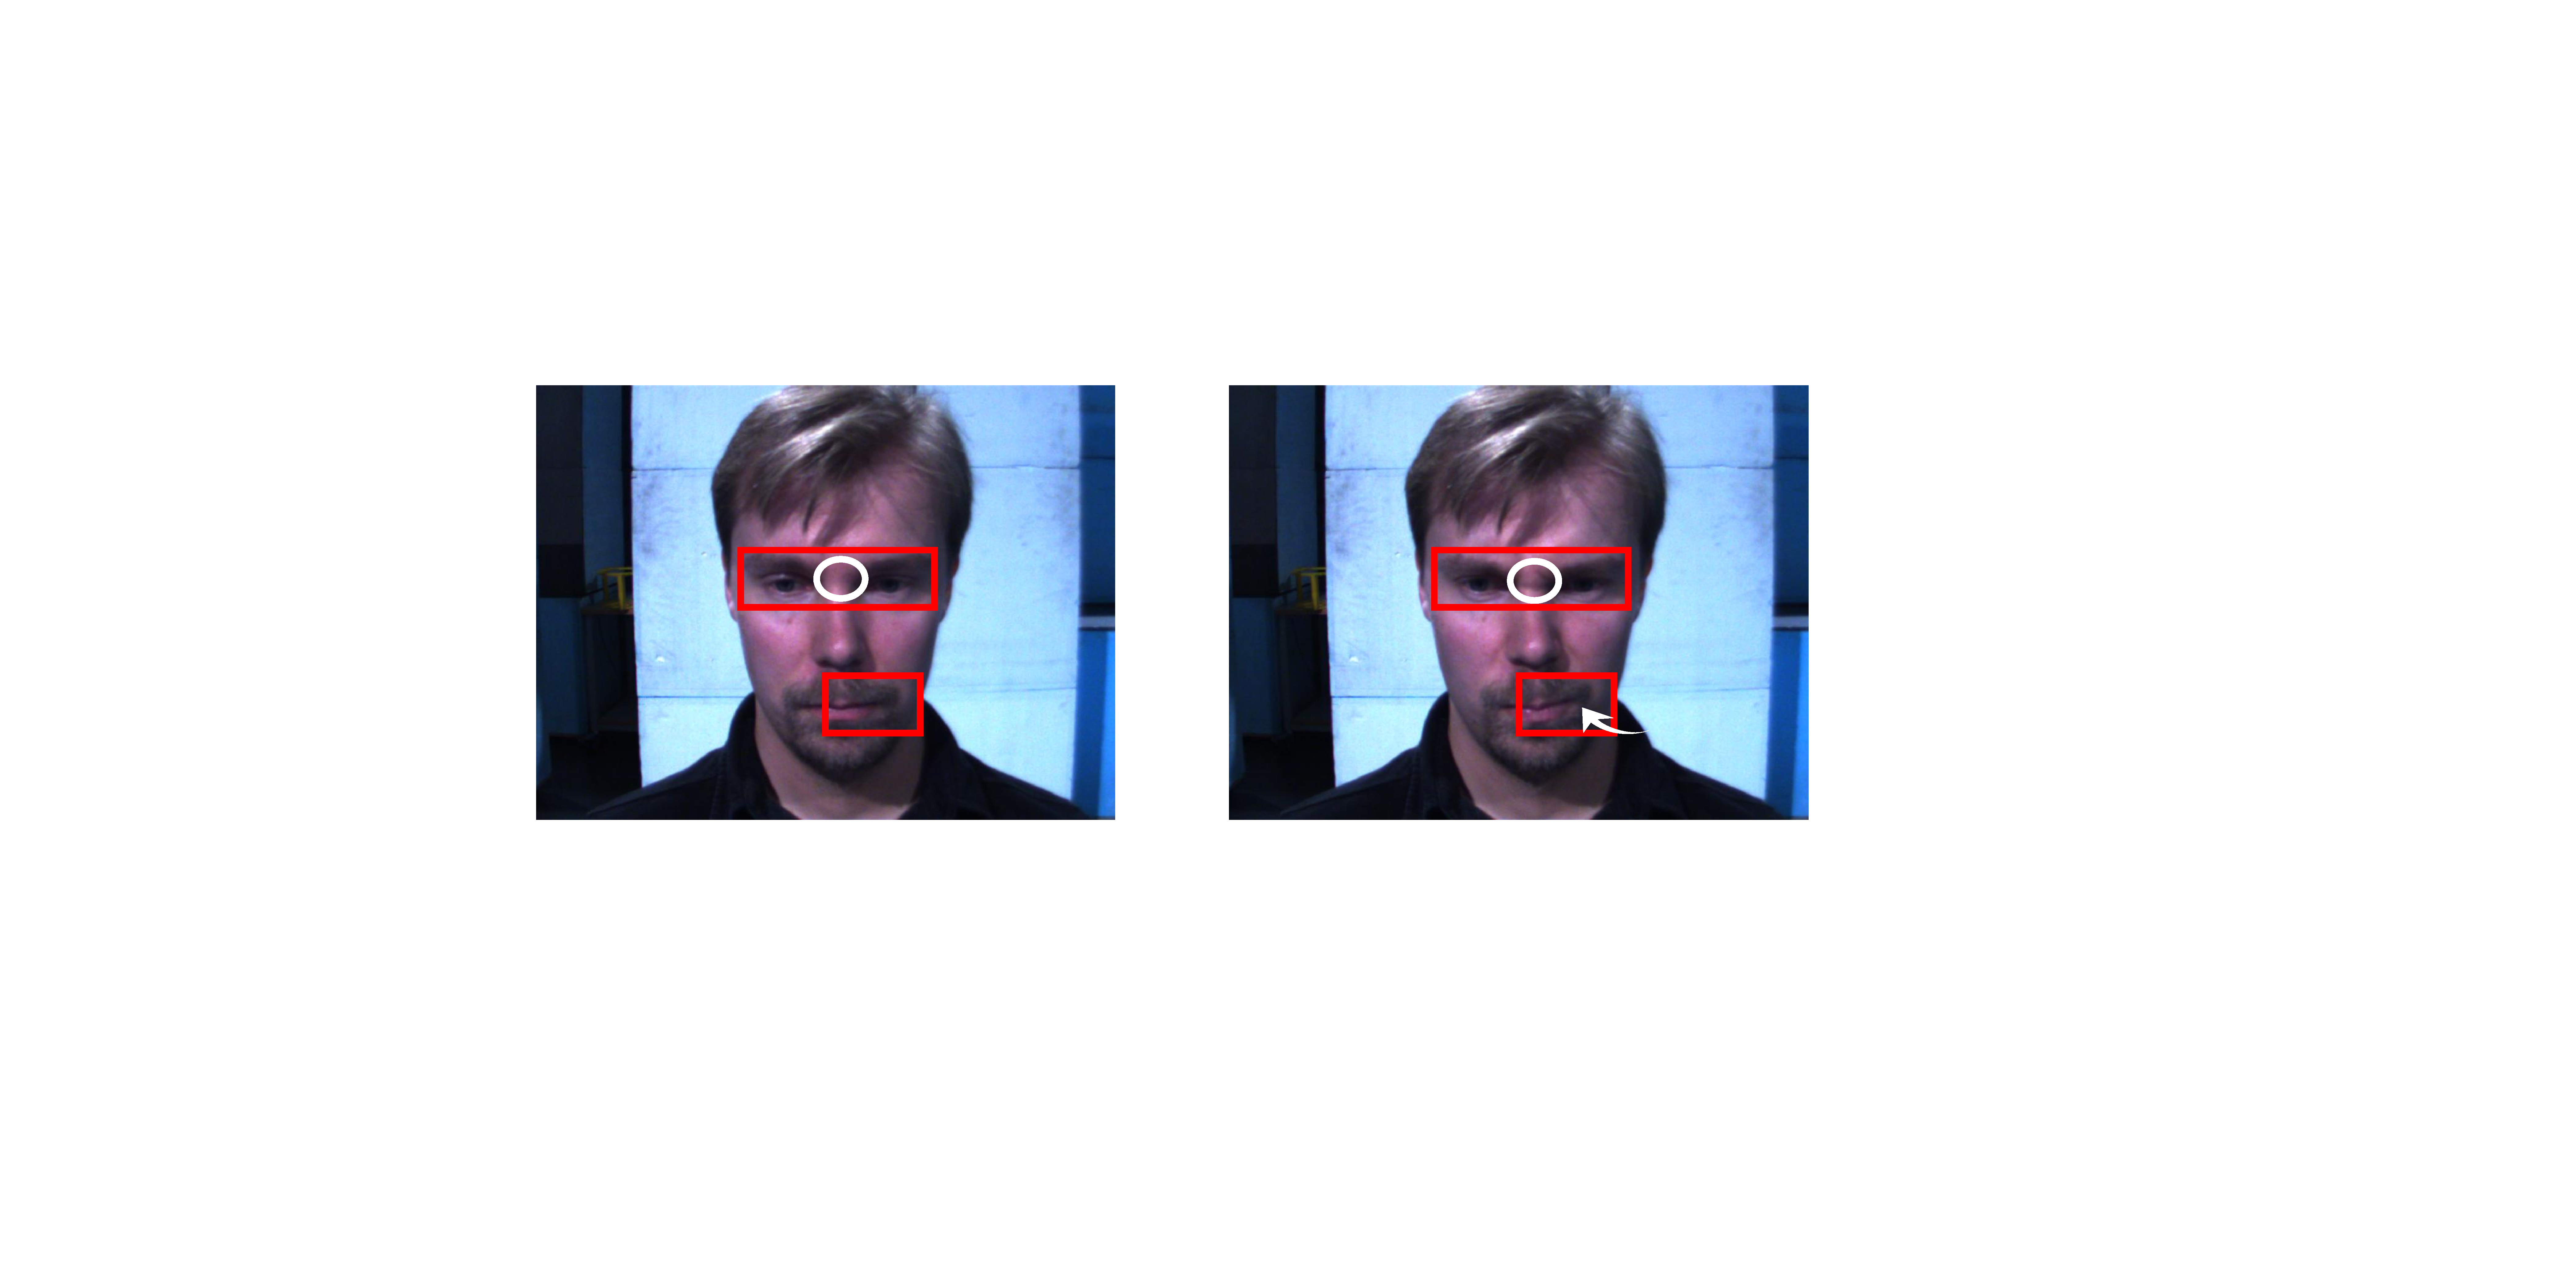
\includegraphics[width=0.65\textwidth]{LR1}
\caption{来自SMIC-HS数据集的两帧}
\label{fig11}
\end{figure}

由于现有的自发微表情数据集中不存在低分辨率的图像序列,所以我们采用图像退化处理的方法来获得模拟的低分辨率微表情图像序列。论文\citepns{wang2014low}将低分辨率图像分为三大类:小尺寸(Small Size)、低质量(Poor Quality)和小尺寸\&低质量(Small Size \& Poor Quality)。我们考虑第三种类型的图像(小尺寸\&低质量)作为模拟图像,这样更接近真实应用的情况。

在图像重建任务中,低分辨率图像序列是通过对高分辨率图像序列进行模糊、下采样和噪声处理得到的\citep{shi2018hallucinating},如下式所示:
\begin{equation}
    \label{eq1}
    \boldsymbol{L} = \boldsymbol{DBH}+\boldsymbol{n}
\end{equation}
其中 $\boldsymbol{D}$和$\boldsymbol{B}$分别是下采样和模糊处理,$\boldsymbol{H}$是高分辨率图像,$\boldsymbol{n}$是加性噪声,$\boldsymbol{L}$是低分辨率图像。我们按照公式~\ref{eq1}的原理对原始数据处理获得实验所需的低分辨率微表情数据,具体如章节\ref{exp}的实验部分所示。

\section{数据预处理}

在我们提出的框架中,预处理主要包括三个步骤:人脸对齐、人脸分割和帧插值处理。原始视频中存在自然的姿势变化和无意识的移动,数据集中收集了不同性别、年龄和种族的参与者的微表情视频片段。因此,为了避免上述非表达因素的干扰,进行人脸对齐和人脸分割是必不可少的。同时,由于微表情的强度是非常微弱的,为了减少类内变化和突出微表情运动产生的类间差异,更需要最小化微表情片段间的其他差异(如人脸大小和人脸形状)。为此,我们使用以下描述方式对所有人脸与模型脸对齐处理。

首先,我们选择一个中性的人脸图像作为模型人脸,使用主动形状模型检测模型脸的68个人脸关键点,接着对第$i$个微表情片段的第一帧上的人脸检测68个关键点,然后使用局部加权平均计算它们之间的关系,对微表情片段的所有帧均使用上述关系进行归一化。最后,将归一化后的图像换算为原始图像的二维变换,根据第一帧中瞳孔的坐标,从每个微表情片段的归一化图像中裁剪出人脸区域。详细过程如下文所示:

\subsection{主动形状模型}

从采集的视频中选取其中没有表情且正面人脸的一帧作为模型脸$\boldsymbol{I_{mod}}$ ,手工定位两只眼睛的位置。然后,利用主动形状模型(Active Shape Model, ASM)检测68个人脸关键点$\boldsymbol{\psi(I_{mod})}$\citep{cootes1995active}。值得注意的是,传统的ASM算法机械地通过检测差异点获取目标,并没有选择目标对错的能力,本章在原算法的基础上增加了条件限定,使得检测的人脸更加准确、规范。如错误标定其他物品或其他人脸(非主要人脸)时,计算任意对应位置关键点的相对距离$\boldsymbol{L(I_{mod})}$ :
\begin{equation}
    \label{eq2}
    \boldsymbol{L^{(i)}(I_{mod})}=\left \| \boldsymbol{\psi_{I_{mod}}}(p\pm 68)-\boldsymbol{\psi_{I_{mod}}}(q\pm 68) \right \|_{2}^{2\displaystyle }
\end{equation}
其中$i$指标定的关键点组数,$p$、$q$指一个关键点组中任意两点,$n$为关键点的个数,数量为68的倍数。选择相对距离$\boldsymbol{L^{(i)}(I_{mod})}$ 最大的一组关键点来确定视频帧中主要人脸。如图~\ref{fig12}所示,1框内为目标人脸,2框为错误识别。通过上述算法在实验过程中错误标定率明显下降。

\begin{figure}[!htbp]
\centering
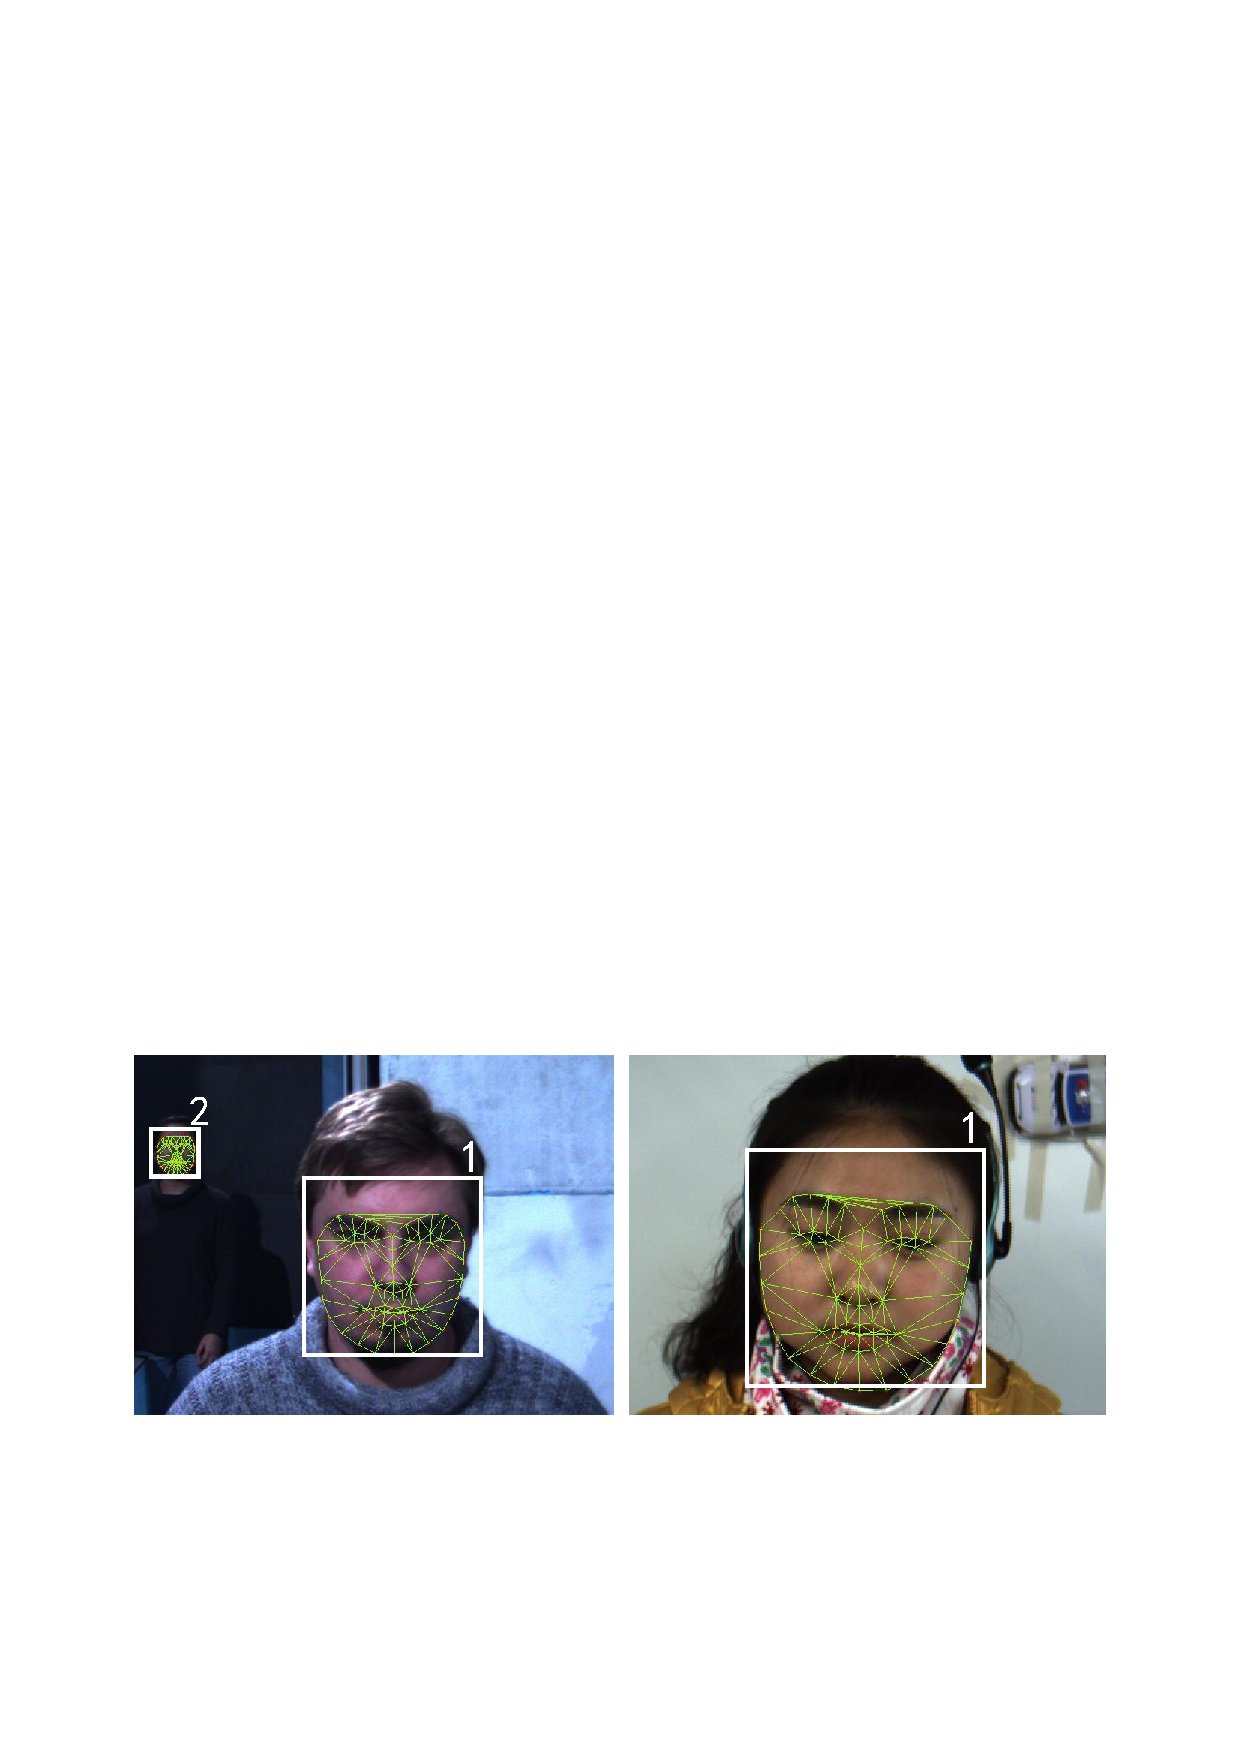
\includegraphics[width=0.70\textwidth]{3LR1}
\caption{ASM算法标定的68个人脸关键点}
\label{fig12}
\end{figure}

\subsection{局部加权平均算法}

对每段个视频的第一帧$\boldsymbol{I_{j,1}}$应用ASM算法标定68个人脸关键点$\boldsymbol{\psi (I_{j,1})}$,使用局部加权平均函数(Local Weighted Mean,LWM)建立模型脸关键点集$\boldsymbol{\psi (I_{mod})}$与视频第一帧关键点集$\boldsymbol{\psi (I_{j,1})}$之间的对应关系\citep{goshtasby1988image}:
\begin{equation}
    \label{eq3}
    \boldsymbol{T_{j}}=LWM(\boldsymbol{\psi (I_{mod})},\boldsymbol{\psi (I_{J,1}))},~~j=1,\cdots ,l
\end{equation}
其中$j$是视频段号,$l$是视频片段总数。对视频片段的所有帧应用该关系,使视频的每一帧具有与模型脸$\boldsymbol{\psi (I_{mod})}$统一的姿态:
\begin{equation}
    \label{eq4}
    \boldsymbol{I_{j,k}^{'}}=\boldsymbol{T_{j}}\times \boldsymbol{I_{j,k}},\quad k=1,\cdots ,n_{j}
\end{equation}
其中$\boldsymbol{I_{j,k}}$为第$j$个视频片段的第$k$帧,$\boldsymbol{I_{j,k}^{'}}$为统一姿态后的第$j$个视频片段的第$k$帧,$n_{j}$为$j$视频片段的帧数。如图~\ref{fig13}所示,两图均按照模型脸统一姿态,左图剔除了错误识别,右图改变了头部的倾斜角度,实验表明通过这种方法大大减少了非表情因素的干扰。

\begin{figure}[!htbp]
\centering
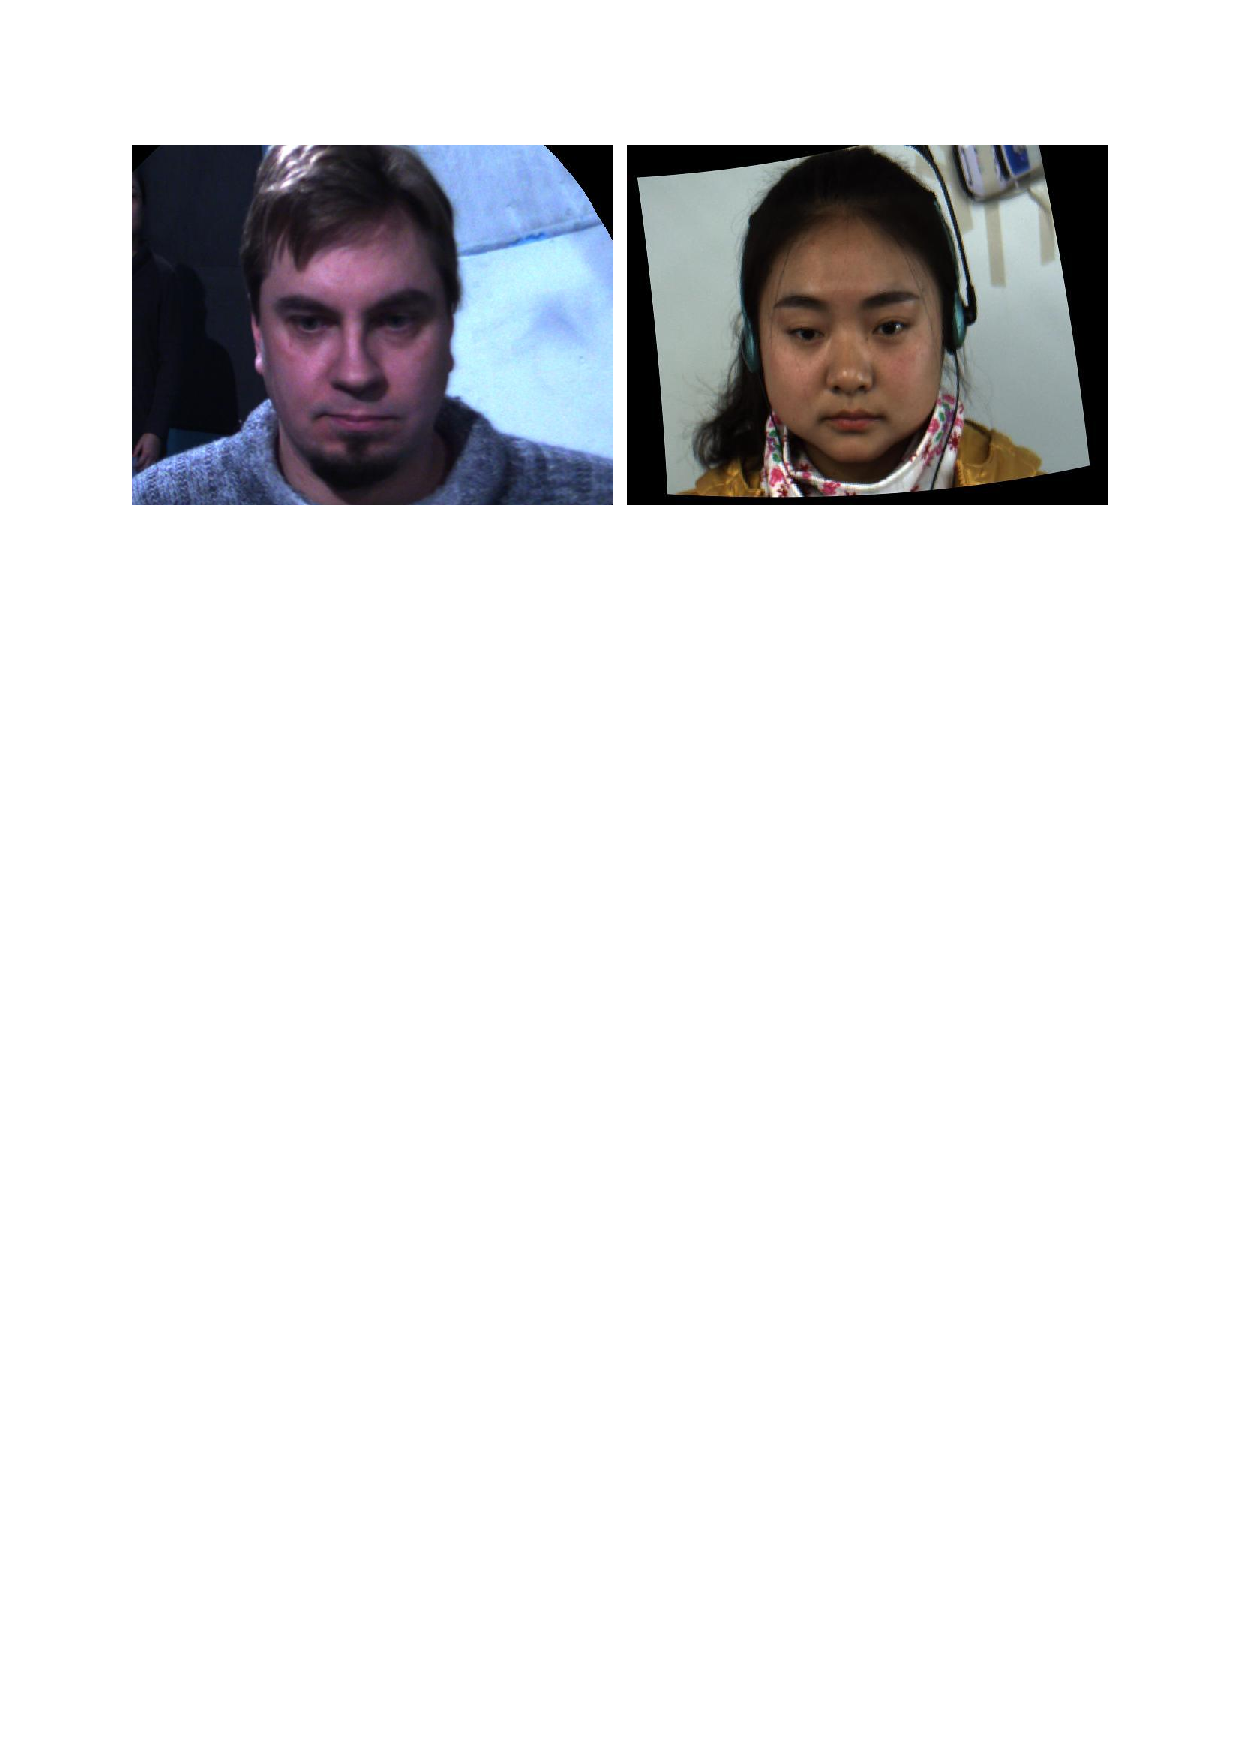
\includegraphics[width=0.70\textwidth]{3LR2}
\caption{LWM算法人脸对齐后的图像}
\label{fig13}
\end{figure}

\subsection{时间插值模型}

微表情识别其中一个特殊的挑战是微表情持续时间短。例如,SMIC数据集中最短的片段持续时间为3/25秒,只有3帧(25 fps)之多。这样的短序列严重限制了许多时空特征描述符的应用,如LBP-TOP特征沿时间维度的可行半径$r$只能为1。除此之外,微表情视频片段之间有不同的长度,而且变化也相当大,从4帧到50帧(如果用100帧/秒的相机拍摄)不等,这也对一些对视频帧数敏感的特征描述符提出了挑战。

Zhou等人在论文\citepns{zhou2011towards}中提出了一种时间插值模型(Temporal Interpolation Model,TIM)。该模型在原论文中用于唇语识别(Lipreading),论文中提到如果我们将一段视频中讲话嘴的运动视为连续过程,则语音视频的图像序列可以被视为沿着表示图像空间中话语的曲线以固定速度采样的一组图像,或更一般地表示为从图像中提取的视觉特征。通常,这样的空间具有高维度,并且我们可以假定存在一个低维流行,其中连续的发声过程可以通过连续和某种确定性函数来表征。根据这样的特性,我们将其一般化地应用到低分辨率环境下微表情识别的框架中,使用TIM方法来解决与微表情持续时间和帧数差异相关的问题。在我们的工作中,我们通过将输入视频表示为路径图$P_{n}$来揭示这样的功能,其中$n$是顶点数。图~\ref{fig14}(a)给出了这种图表示例,如图所示,每个顶点对应于一个帧,并且顶点之间的连接可以由邻接矩阵$\boldsymbol{W}\in \left \{ 0,1 \right \}^{n\times n}$ 表示,其中当$\left | i-j \right |= 1,~ i,j=1,2,\cdots ,n$时$W_{ij}= 1$,否则为0。

\begin{figure}[!htbp]
    \centering
    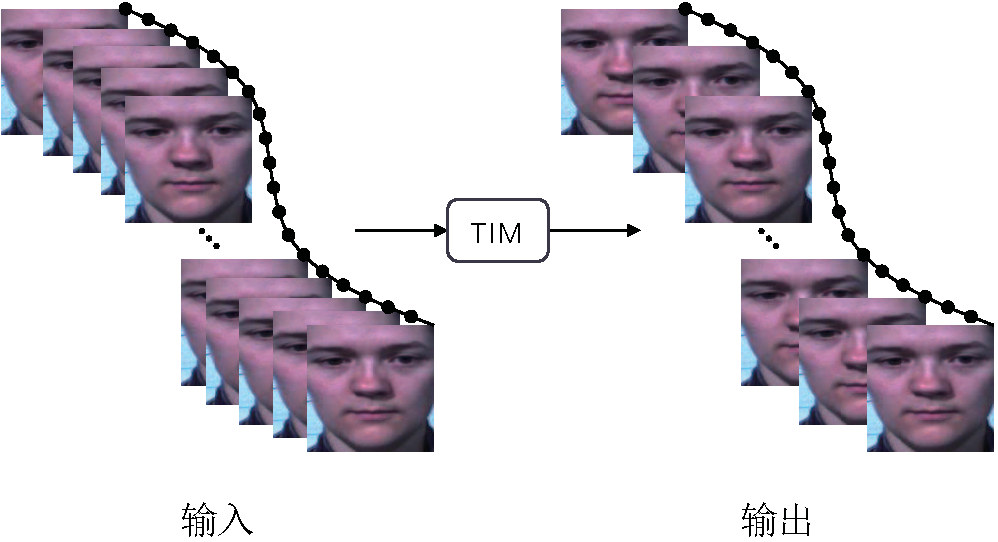
\includegraphics[width=0.9\textwidth]{LR2}
    \begin{spacing}{1.0}
    \caption{TIM方法映射过程}
    \label{fig14}
    \centerline{\footnotesize \textmd{(a)共19帧的图像序列插值过程($P_{19}$ ),输入为原始图像,输出为插值后图像;}}
    \centerline{\footnotesize \textmd{(b)-(d)为图像序列的Laplacian第1、第9和第18特征向量的映射。}}
    \end{spacing}
\end{figure}

在本文中对由重建出的高分辨率图像组成的图像序列应用TIM算法统一帧数:将重建的图像序列映射到一条非线性曲线上$\mathcal{F}^{n}:\left [ 1/n,1 \right ]\rightarrow \mathbb{R}^{n-1}$ ,
\begin{equation}
    \label{eq5}
    \mathcal{F}^{n}(t)=\begin{bmatrix}f_{1}^{n}(t)\\ f_{2}^{n}(t)\\ \vdots \\ f_{n-1}^{n}(t)\end{bmatrix}
\end{equation}
其中$f_{k}^{n}(t)=sin(\pi kt+\pi (n-k)/n),\quad t\in \left [ 1/n,1 \right ]$ ,$n$为视频段中帧数(图像序列个数),根据实验需求等间距采样,获得统一帧数。

TIM方法通过路径图来描述帧序列的结构:学习图像序列特定的映射以连接图像序列中的帧和嵌入在路径图中的曲线,从而将图像序列投影到路径图中,如图~\ref{fig14}(a)所示。图~\ref{fig14}(b)-(d)的曲线是[0,1]区间内单个变量$t$的连续确定性函数,控制着帧间的时间关系。在微表情的连续过程中出现的不可见的帧也可以用曲线来表征。因此,使用TIM方法,无论是向下采样还是向上采样,通过控制变量$t$在不同时间点的变化,我们都可以将帧序列改变为任意长度。

在本文提出的框架中,TIM方法被用来将所有的微表情片段(数据集)插为一个固定的长度,例如,10帧、20帧或40帧。这样既可以解决持续时间短的问题,也可以解决序列长度不统一的问题。当前步骤的目的一方面可以在选择特征参数时提供更多的选项,另一方面利用时空特征描述符实现更稳定的性能。如何选择最合适的TIM插值长度的问题在论文\citepns{Li2017Towards}中进行了探讨和讨论,本文将其讨论结果作为参考,具体如章节\ref{exp}的实验部分所述。

\section{超分辨重建过程}

在本文中,我们分别提出了基于块和基于像素的两种新的正则化,它们可以有效地将输入的低分辨率人脸图像重建成高分辨率人脸图像。与依赖于低分辨率和高分辨率空间中局部几何一致性假设的传统基于块的模型不同,所提出的方法直接规范了目标块与高分辨率空间中相应训练集之间的关系。它避免了处理在不同分辨率下保留局部几何结构的棘手问题。利用核函数有效地描述内在特征,我们在高维核空间进一步进行基于块的模型重建,以捕获非线性特征。同时,提出了一种基于像素的模型来规范局部邻域中像素的关系,可以用来增强目标高分辨率人脸图像中的模糊细节。它主要是沿着结构的主导方向重建像素,这对于保留复杂边缘上的高频信息是有用的。最后,我们将两个重建模型组合成一个统一的框架。可以通过执行迭代过程来最终优化输出重建的高分辨率人脸图像。实验结果表明,所提出的人脸Hallucination方法比现有技术方法具有更好的性能。

重建模型$\mathbf{L=DBH}+\varepsilon$ 中的高分辨率人脸图像$\mathbf{H}$严重欠定,意味着每个低分辨率人脸图像对应于无限多个高分辨率估计。为了改善这个问题,必须在整个重建过程之前加入进一步的正则化。通过附加先验条件,可以获得高分辨率人脸图像$\mathbf{H}$的唯一解决方案。重建模型可以表示为:
\begin{equation}
    \label{eq6}
    \mathbf{H} = \mathrm{arg}~\underset{\mathbf{H}}{\mathrm{min}}\left \{ \left \| \mathbf{L-DBH} \right \| _{2}^{2}+\gamma R(\mathbf{H}) \right \}
\end{equation}
其中$R(\mathbf{H})$表示正则化模型,$\gamma$是平衡重建误差和正则化项的相应参数。在\ref{eq6}中,第一项确保了估计的高分辨率人脸图像和观察到的低分辨率人脸图像的一致性,而附加的先验项进一步规范了高分辨率人脸图像的局部细节。根据人脸图像的特点,提出了两种有效的正则化模型,以约束重建过程。以下将描述上述两个先验项的细节。

低分辨率图像和高分辨率图像在质量和分辨率上都是不同的。高分辨率图像序列的微表情识别方法不能直接应用于低分辨率图像序列。在2.1节中,我们介绍了从高分辨率图像生成低分辨率图像的过程。

为了重建高分辨率图像,论文\citepns{shi2018hallucinating}提出了一种新的人脸幻觉算法。将基于块的正则化项与基于像素的正则化项相结合,对目标函数进行约束。重构后的高分辨率图像$\boldsymbol{H}$可以通过最小化以下目标函数得到:
\begin{equation}
 \label{eq7}
 \begin{split}
    f\left ( \boldsymbol{H} \right )= \left \| \boldsymbol{L}-\boldsymbol{DBH} \right \|{_{2}^{2}}+\alpha \boldsymbol{F}_{patch}+\eta \boldsymbol{F}_{pixel}+\lambda \boldsymbol{F}_{penalty}
 \end{split}
\end{equation}
其中右侧第一项为重建误差,后三项分别是基于块的正则项、基于像素的正则项以及惩罚项。图~\ref{fig15}展现了重建工作的具体流程。具体将在下文详细介绍。

\begin{figure}[!htbp]
\centering
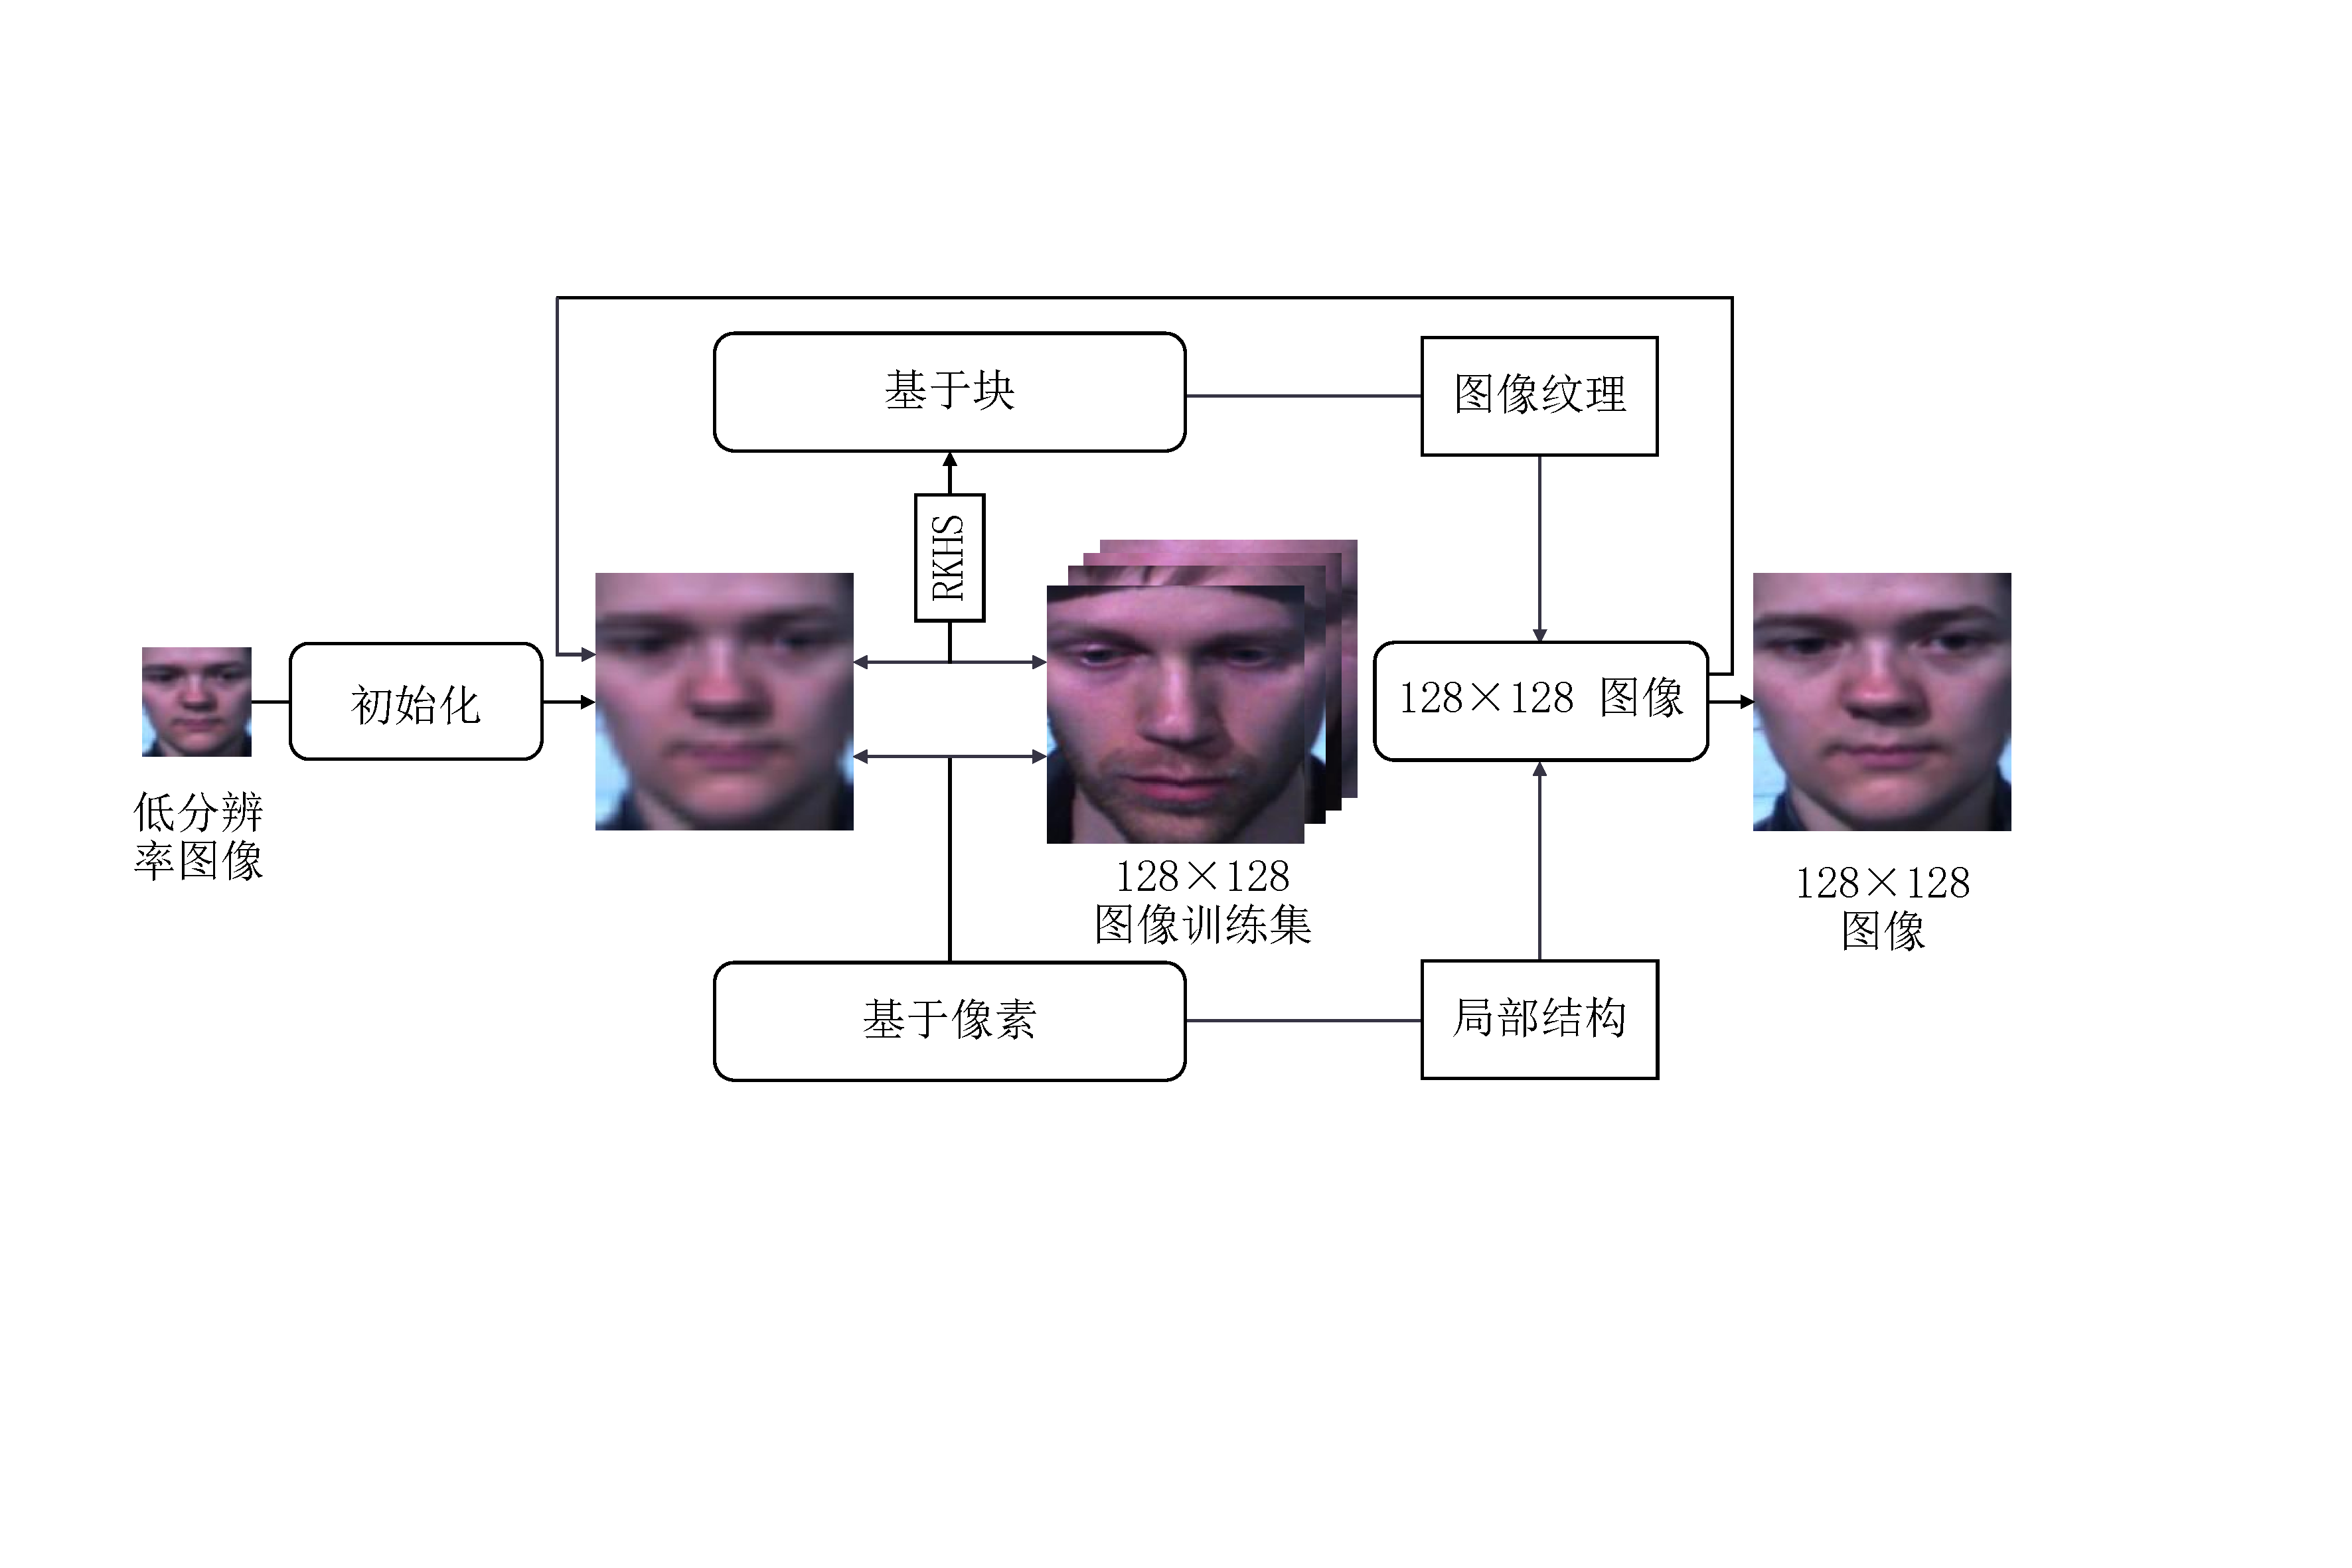
\includegraphics[width=0.75\textwidth]{LR3}
\caption{超分辨重建过程}
\label{fig15}
\end{figure}

\subsection{基于的块方法}

将分割后的图像$\boldsymbol{L}$(低分辨率图像)应用三线性插值法调整为与训练样本图像$\boldsymbol{H}$(高分辨率图像,来自公开的高分辨率图像集)大小相等的尺寸,将此图命为$\boldsymbol{H^{(0)}}$(超分辨重建过程的初始图像),对图像分块处理(如分块数为$8\times8$),如图7所示,最小化代价函数:
\begin{equation}
 \label{eq8}
 \begin{split}
   \boldsymbol{J_{\tau }(\omega _{\tau },H^{(k)})} & =\left \{ \left \| \boldsymbol{\phi (R_{\tau }H^{k})}-\boldsymbol{\phi (H_{\tau })\omega _{\tau }} \right \| _{2}^{2}+\boldsymbol{\lambda} \left \| \boldsymbol{d_{\tau }}\bigotimes \boldsymbol{\omega _{\tau }} \right \|_{2}^{2}\right \} \\
   \boldsymbol{s.t. 1^{T}\omega _{\tau }}= 1 & ,2,\cdots ,M
 \end{split}
\end{equation}
估算结合系数$\boldsymbol{\omega _{\tau }}$ ,将其初始结合系数命名为$\boldsymbol{\omega_{\tau }^{0}}$,此时$\boldsymbol{H^{(k)}}$ 已知,即$\boldsymbol{H^{(0)}}$ ,其中$\boldsymbol{\tau}$为图像中图像块的位置,$\boldsymbol{R_{\tau }}$为提取所有图像集位置$\tau$的图像块的矩阵, $\boldsymbol{H_{\tau }}=\left [ h_{\tau }^{1},\cdots ,h_{\tau }^{N} \right ]$为高分辨率图像位置$\boldsymbol{\tau}$处图像块集($N$为训练样本的数量,即高分辨率图像集的数量),$\boldsymbol{\phi (\cdot )}$ 为从原始空间到无限维再生核希尔伯特空间(Reproducing Kernel Hilbert Space, RKHS)的映射,$\boldsymbol{d_{p}}$ 描述了目标高分辨率块(重建出的块)与相应的训练样本块在核映射空间的核相似性,$\bigotimes$ 表示哈达玛积,$\boldsymbol{\lambda}$为惩罚系数,$\boldsymbol{1}$为全为1的列向量,$M$为图像的块数。

\subsection{基于像素的方法}

可以通过解决上述优化问题(25)来获得最终的高分辨率人脸图像$\boldsymbol{H}$。但是,目标函数是非凸优化问题,很难直接获得全局最优解。幸运的是,我们可以期望通过迭代过程获得局部最优解。为了解决(25)中的问题,我们可以分别优化$\omega _{\tau }$和$\boldsymbol{H}$,同时固定另一个值。例如,如果$\omega _{\tau }$的值是固定的,则可以通过最小化以下函数来获得最优$\boldsymbol{H}$:
\begin{equation}
 \label{eq9}
 \begin{split}
   \boldsymbol{f(H)}= \left \| \boldsymbol{L^{k}}-\boldsymbol{DBH^{k}} \right \|_{2}^{2}+\boldsymbol{\eta \sum_{\tau }}\left \| \boldsymbol{x_{\tau }h^{k}}-\boldsymbol{\beta _{\tau }H_{\tau }} \right \|_{2}^{2}+ \\
   \boldsymbol{\alpha \sum_{\tau }}(\left \| \boldsymbol{\phi (R_{\tau }H^{k})}-\boldsymbol{\phi (H_{\tau })\omega _{\tau } }\right \|_{2}^{2}+ \boldsymbol{\lambda} & \left \| \boldsymbol{d_{\tau }}\bigotimes \boldsymbol{\omega _{\tau } }\right \|_{2}^{2})+\boldsymbol{\sigma MSE} \\
   \boldsymbol{s.t. \quad 1^{T}\omega _{\tau }}= 1,2,\cdots ,M \qquad \qquad \qquad \qquad \qquad \quad &
 \end{split}
\end{equation}
获得重建的高分辨率图像$\boldsymbol{H^{(k)}}$(初始结果命名为$\boldsymbol{H^{(1)}}$),其中$\boldsymbol{D}$为下采样矩阵,$\boldsymbol{B}$为模糊处理矩阵,$\boldsymbol{\beta _{\tau }}$为规范全局优化的像素间关系矩阵,$\boldsymbol{MSE}$为均方误差,$\boldsymbol{\eta }$为基于像素的正则项系数,$\boldsymbol{\alpha}$为基于块的正则项系数,$\boldsymbol{\sigma}$为均方误差的系数。

基于块的模型可以恢复人脸图像的大多数高频纹理。然而,局部结构需要进一步考虑抑制复杂边缘上的伪像。其目的在于表征相邻像素之间的关系以增强边缘结构,这在基于块的先验项中未被考虑。

通过交替优化公式~\ref{eq9}和公式~\ref{eq8}来解决目标函数。因此,它需要对两个目标函数进行初始估计,以便开始迭代。我们首先利用低分辨率图像特征来代替公式~\ref{eq8}中高分辨空间的相应特征,这给出了对$\omega _{\tau }$初始值的粗略估计。在初始化之前,通过双三次插值将低分辨率图像放大到与高分辨率相同的大小,以获得更多的高频信息。我们还简单地将低分辨率$\boldsymbol{L}$的插值结果视为高分辨率人脸图像$\mathbf{H}^{(0)}$ 的初始估计。

利用两个目标的初始值,我们可以通过最小化公式~\ref{eq9}来优化输出高分辨率图像$\boldsymbol{H}$。一旦完成,通过求解公式~\ref{eq8}获得每个位置的组合系数$\omega _{\tau }$。我们重复迭代过程以更新上述目标,直到优化问题(25)收敛到局部最小值。最后,获得最优解$\boldsymbol{H}$作为输出高分辨率人脸图像。算法1总结了完整面部幻觉程序的细节。

在本文中,我们提出了两种新的正则化模型来处理低分辨率人脸模糊问题。基于块的模型规范了高分辨率空间中目标块和训练块之间的关系,这有效地恢复了局部纹理。与以前在低分辨率空间中建立正则化的方法不同,它避免了保持局部几何一致性的困难。此外,高分辨率块片被投射到RKHS中,这有助于寻求重建中的非线性关系。基于像素的模型被设计用于补偿局部细节,尤其是眼睛、鼻孔和嘴部区域。它沿着结构的主导方向对像素进行重建,这对于重建局部边缘结构是有效的。通过组合上述两种正则化模型,可以最终优化整个高分辨率图像。实验结果表明,与各种条件下的现有基线相比,所提出的方法产生了优异的结果。

\section{微表情的特征提取与分类}

如章节\ref{chap:relate}所述,时空描述符是微表情分析研究的主流。如图~\ref{fig10}所示,微表情识别主要分为两部分:特征提取和分类。本文提出的微表情识别框架使用LBP-TOP时空特征和线性支持向量机分类器。

在以往的微表达分析方法中研究人员展示了LBP-TOP及其变体作为特征描述符的优势。与传统的基于单个图像的LBP特征不同,LBP-TOP可以捕捉到空间和时间域的动态变化,这对于微表情识别是必不可少的。在分类部分,我们使用LSVM作为分类器。为了进行公平的比较,我们在实验中采用了Leave-one-subject-out协议。

\subsection{LBP-TOP特征提取}

LBP-TOP由Zhao \& Pietik{\"a}inen在论文\citepns{zhao2007dynamic}中提出。LBP-TOP是原LBP的扩展,用于时空域的动态纹理分析。根据章节\ref{chap:relate}的相关工作中的描述,LBP-TOP及其变体是目前微表情识别研究中最常用的特征。

视频序列可以看作是X、Y和T维上像素的长方体,传统的LBP代码可以从XY、XT或YT平面中提取特征直方图,如图~\ref{fig16}中$\textrm{LBP-TOP}^{1}$所示(图中的红色立方体)。为了总结三维长方体的时空属性,将每个平面的三个LBP直方图拼接成一个大直方图作为最终的LBP-TOP特征向量,如图~\ref{fig16}中$\textrm{LBP-TOP}^{2}$所示,关于Blocksize的划分将在章节\ref{chap:owner1}中讨论。

按照这种方法我们首先将整个人脸图像序列划分为几个长方体,如$ 5\times5\times1 $,$ 8\times8\times2 $等,其中前两个参数决定了空间域中的块数,最后一个参数是时间方向上的块数。每个长方体都可以看作一个新的单元,从新单元中三个不同的正交平面(XOY、XOT、YOT)提取LBP特征,我们遍历所有长方体,得到图像序列的LBP-TOP特征,然后将每个长方体的LBP-TOP特征串联起来。

\begin{figure}[!htbp]
    \centering
    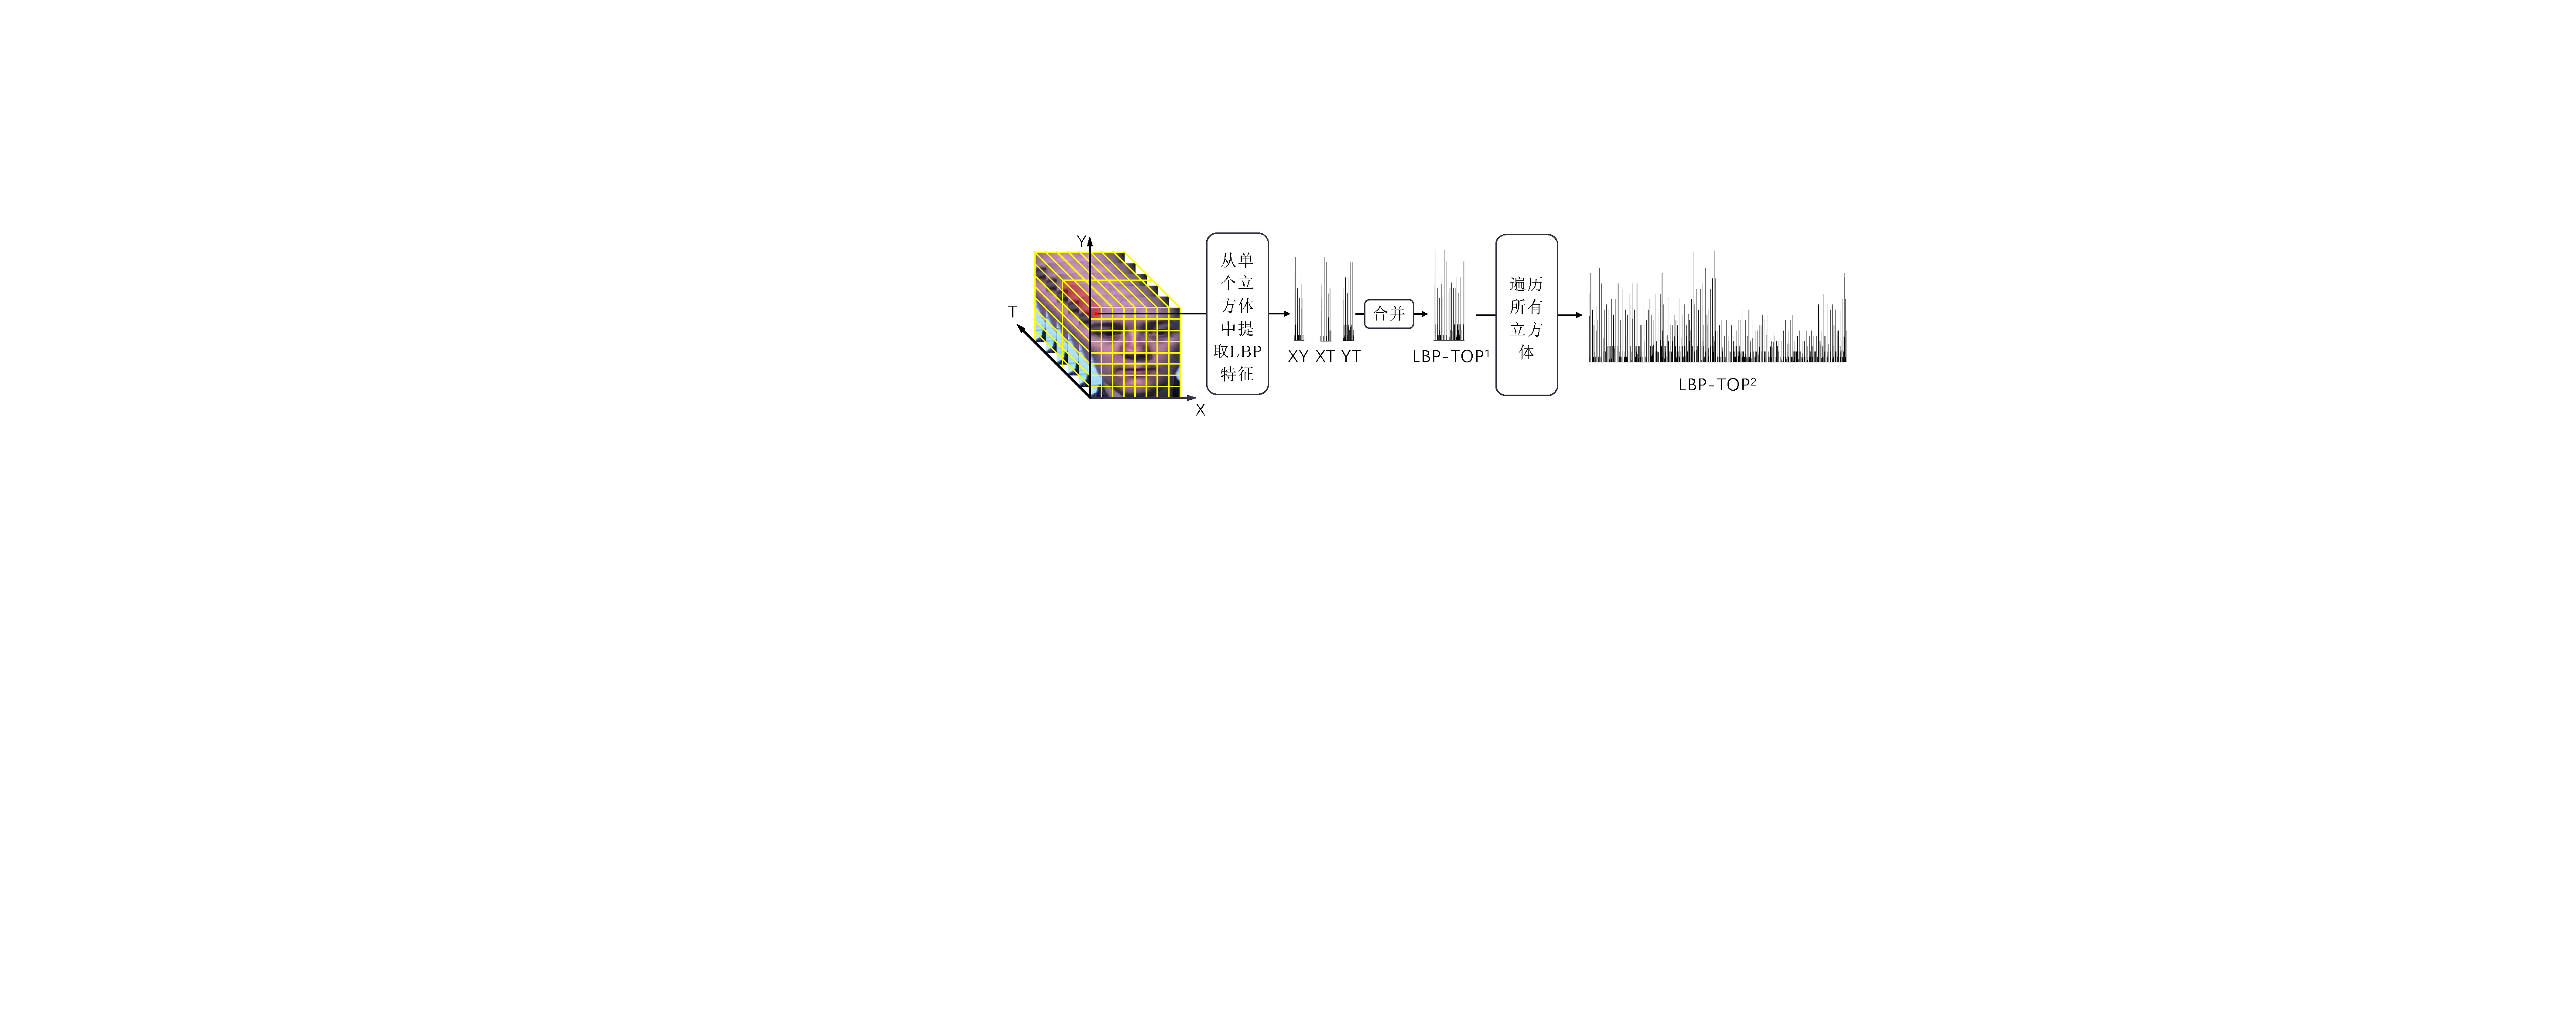
\includegraphics[width=0.9\textwidth]{LBP1}
    \caption{LBP-TOP特征提取过程}
    \label{fig16}
\end{figure}

\subsection{线性支持向量机及交叉验证}

支持向量机(Support Vector Machine,SVM)是一类按监督学习方式对数据进行分类的广义线性分类器,它在解决小样本、非线性及高维模式中有许多特有的优势。SVM的关键在于核函数,采用不同的核函数就会有不同的SVM分类结果。常用到的核函数有线性核(Linear Kernel)、卡方核(Chi-square Kernel)、直方图交叉核(Histogram Intersection kernel)。SVM从90年代后期开始在很多领域均有举足轻重的应用,是曾经打败神经网络的分类方法,近年来,由于深度学习的兴起,SVM的风光开始衰退,但是其仍然不失为一种经典的分类方法。

虽然分类器的选择也很重要,但它并不是目前研究的主要目的。为了保持良好的控制,并将更多的注意力放在框架的前几个步骤上,在接下来的微表情识别实验中,我们使用了线性支持向量机(Linear Support Vector Machine, LSVM)作为分类器\citep{chang2011libsvm},使用leave-one-subject-out协议进行验证。根据数据集发布方提供的微表情表签,我们将来自SMIC的样本分为三类(Positive、Negative、Surprise),来自CASME II的样本分为五类(Happiness、Surprise、Repression、Disgust、Other)。下面将简单描述它们的细节,并将在章节\ref{exp}中提供最终的实验数据。

% 本文讨论线性可分的支持向量机,详细推导其最大间隔和对偶问题的原理。简单起见,以二分类为例,如下图,设训练集为D={(x1,y1),...,(xn,yn)}D={(x1,y1),...,(xn,yn)},蓝色圆点为一类,红色方块为另一类,分类的目标是寻找一个超平面,将两类数据分开。在二维平面中,分类超平面就是一条直线,从图中可以看出,能将训练样本分开的超平面有很多可能(图中绿色虚线),超平面除了要将训练集中的数据分开,还要有较好的泛化性能,需要把测试集中的数据也划分开。从直观上看,绿色实线是比较好的一个划分,因为该直线距离两类数据点均较远,对于数据局部扰动的容忍性较好,能够以较大的置信度将数据进行分类。

交叉验证是用来验证分类器性能的一种统计分析方法。其基本思想是将样本数据集分成两个子集,一个子集用于训练分类器称为训练集,另一个子集用于验证分析分类器的有效性称为测试集。其利用测试集来测试训练得到的分类器,以此作为分类器的性能指标。常用的方法有简单交叉验证、K折交叉验证和leave-one-subject-out(LOSO)交叉验证。LOSO交叉验证方法每次选择一位受试者的所有视频序列作为测试样本,其余$n$个受试者的所有视频序列作为训练样本,重复$n+1$次实验,计算$n+1$次的平均分类识别率。所以LOSO交叉验证方法的样本利用率最高,适合小样本的分类计算。故运用LOSO交叉验证方法对不同核函数的SVM分类器进行微表情的分类实验可以得到更为准确的结果。

\section{实验设置及分析}
\label{exp}

该框架在SMIC和CASMEII两个数据库上进行了测试。为了探究框架中每个单独步骤的效果,我们针对不同的目的分别进行了四个子实验。子实验及其结果如下所述。

TIM插值的效果

在第一个子实验中,我们想要评估插值过程将如何影响框架的性能。我们也希望找到一个合适的序列长度(或长度范围),这将有效的提升微表情识别任务。

原始微表情片段的平均序列长度:SMIC-HS为33.7帧,SMIC-VIS为9.66帧,SMIC-NIR为9.66帧。为了避免其他因素的影响,将重点放在TIM过程上,我们跳过了运动放大的步骤,只使用LBP-TOP(参数固定为$8\times8\times1$个block,$r = 2$,$p = 8$)作为特征描述符。在TIM步骤中我们选择8个插值长度(10、20、…),对SMIC-HS、SMIC-VIS和SMIC-NIR数据集的框架进行评估。

测试结果如图6所示。研究结果可以归纳为两个方面。首先,插值到10帧(简称TIM10)比不使用TIM过程的性能要好得多。与原始序列相比,TIM10几乎没有改变SMIC-VIS和SMIC-NIR的平均序列长度,但是SMIC-HS的下采样过程。因此,我们认为序列长度的统一导致了性能的提高。其次,如果我们将TIM10的结果与较长的TIM序列的结果进行比较,就会发现较长的插值序列并不会带来更好的性能。对这个结果的一种可能的解释是,如果微表情片段被插值成更长的序列,时间维度的变化就会被稀释。根据这两个发现,对于目前的框架来说,TIM为10帧似乎是最好的选择。在接下来的所有实验中,如果没有另外指定,TIM10将作为默认值应用于框架中。

特征的比较

第二个子实验的目的是比较三个特征的性能。在每个特征的三个正交平面上分别计算五种直方图组合。

人脸对齐后,应用TIM10对所有序列进行10帧插值。在后面的讨论中暂时跳过了运动放大步骤。从不同参数序列的均匀分割块中提取三种特征。对于LBP特征,我们改变半径$r$,邻点$p$和划分块数;对于HOG和HIGO特性,我们将bin的数量固定为$b = 8$,并改变划分块的数量。对SMIC和CASMEII的三个数据集进行了测试,结果如表5所示。注意,每个特征的三个正交平面的五个组合的结果被单独列出。对于每个特征组合(表中的一个单元格),只列出所有参数组合中获得的最佳结果(具有相应的参数)。

从结果表中可以发现两个现象。首先,最上面的组合(三个正交平面)并不总是带来最好的性能,特别是对于HIGO特性。在许多情况下,仅使用XOT、YOT或XYOT计划特性就可以获得更好的结果,对于所有四个数据集都是如此。另一方面,XY平面特征总是比其他平面组合得到最低的性能。结果表明,T维上的动态变化是微表情识别中最重要的信息,而XY平面特征所携带的面部特征信息更多,这可能是微表情识别任务中多余的信息,Davison等人也提出了类似的发现。其次,比较这三种特征,基于梯度的特征HOG和HIGO在四个测试数据集中的三个(SMIC-NIR除外)上优于LBP。HIGO的性能似乎略优于HOG,在SMIC上使用HIGO-XOT获得的最高性能为76.06\%。一种可能的解释是HIGO特征不受局部梯度大小的影响,局部梯度大小可能由于微表情片段中肌肉运动速度的多样性而变化。近红外数据显示了另一种趋势。近红外相机记录的皮肤纹理不同于可视彩色视频。对于SMIC-NIR数据集,LBP特征优于其他两个特征,这与Zhao等(2011)之前的研究结果一致。

\begin{table}[!htbp]
  \renewcommand\arraystretch{1.5}
  \centering
  \caption{实验中使用的数据集}
  \label{tab4}
  \begin{tabular}{c|ccc}
    \hline
    & SMIC-HS & SMIC-subHS & CASME II \\ \hline
    微表情数 & 164 & 71 & 247 \\
    参与者 & 16 & 8 & 26 \\
    分类 & 3 & 3 & 5 \\ \hline
  \end{tabular}
\end{table}

我们现在在三个不同的自发微表达数据集上展示实验和结果,即SMIC-HS, SMIC-subHS和CASME II。实验参数的设置和结果分析将在下面的小节中讨论。

\begin{figure}[!htbp]
    \centering
    \begin{subfigure}[b]{0.35\textwidth}
      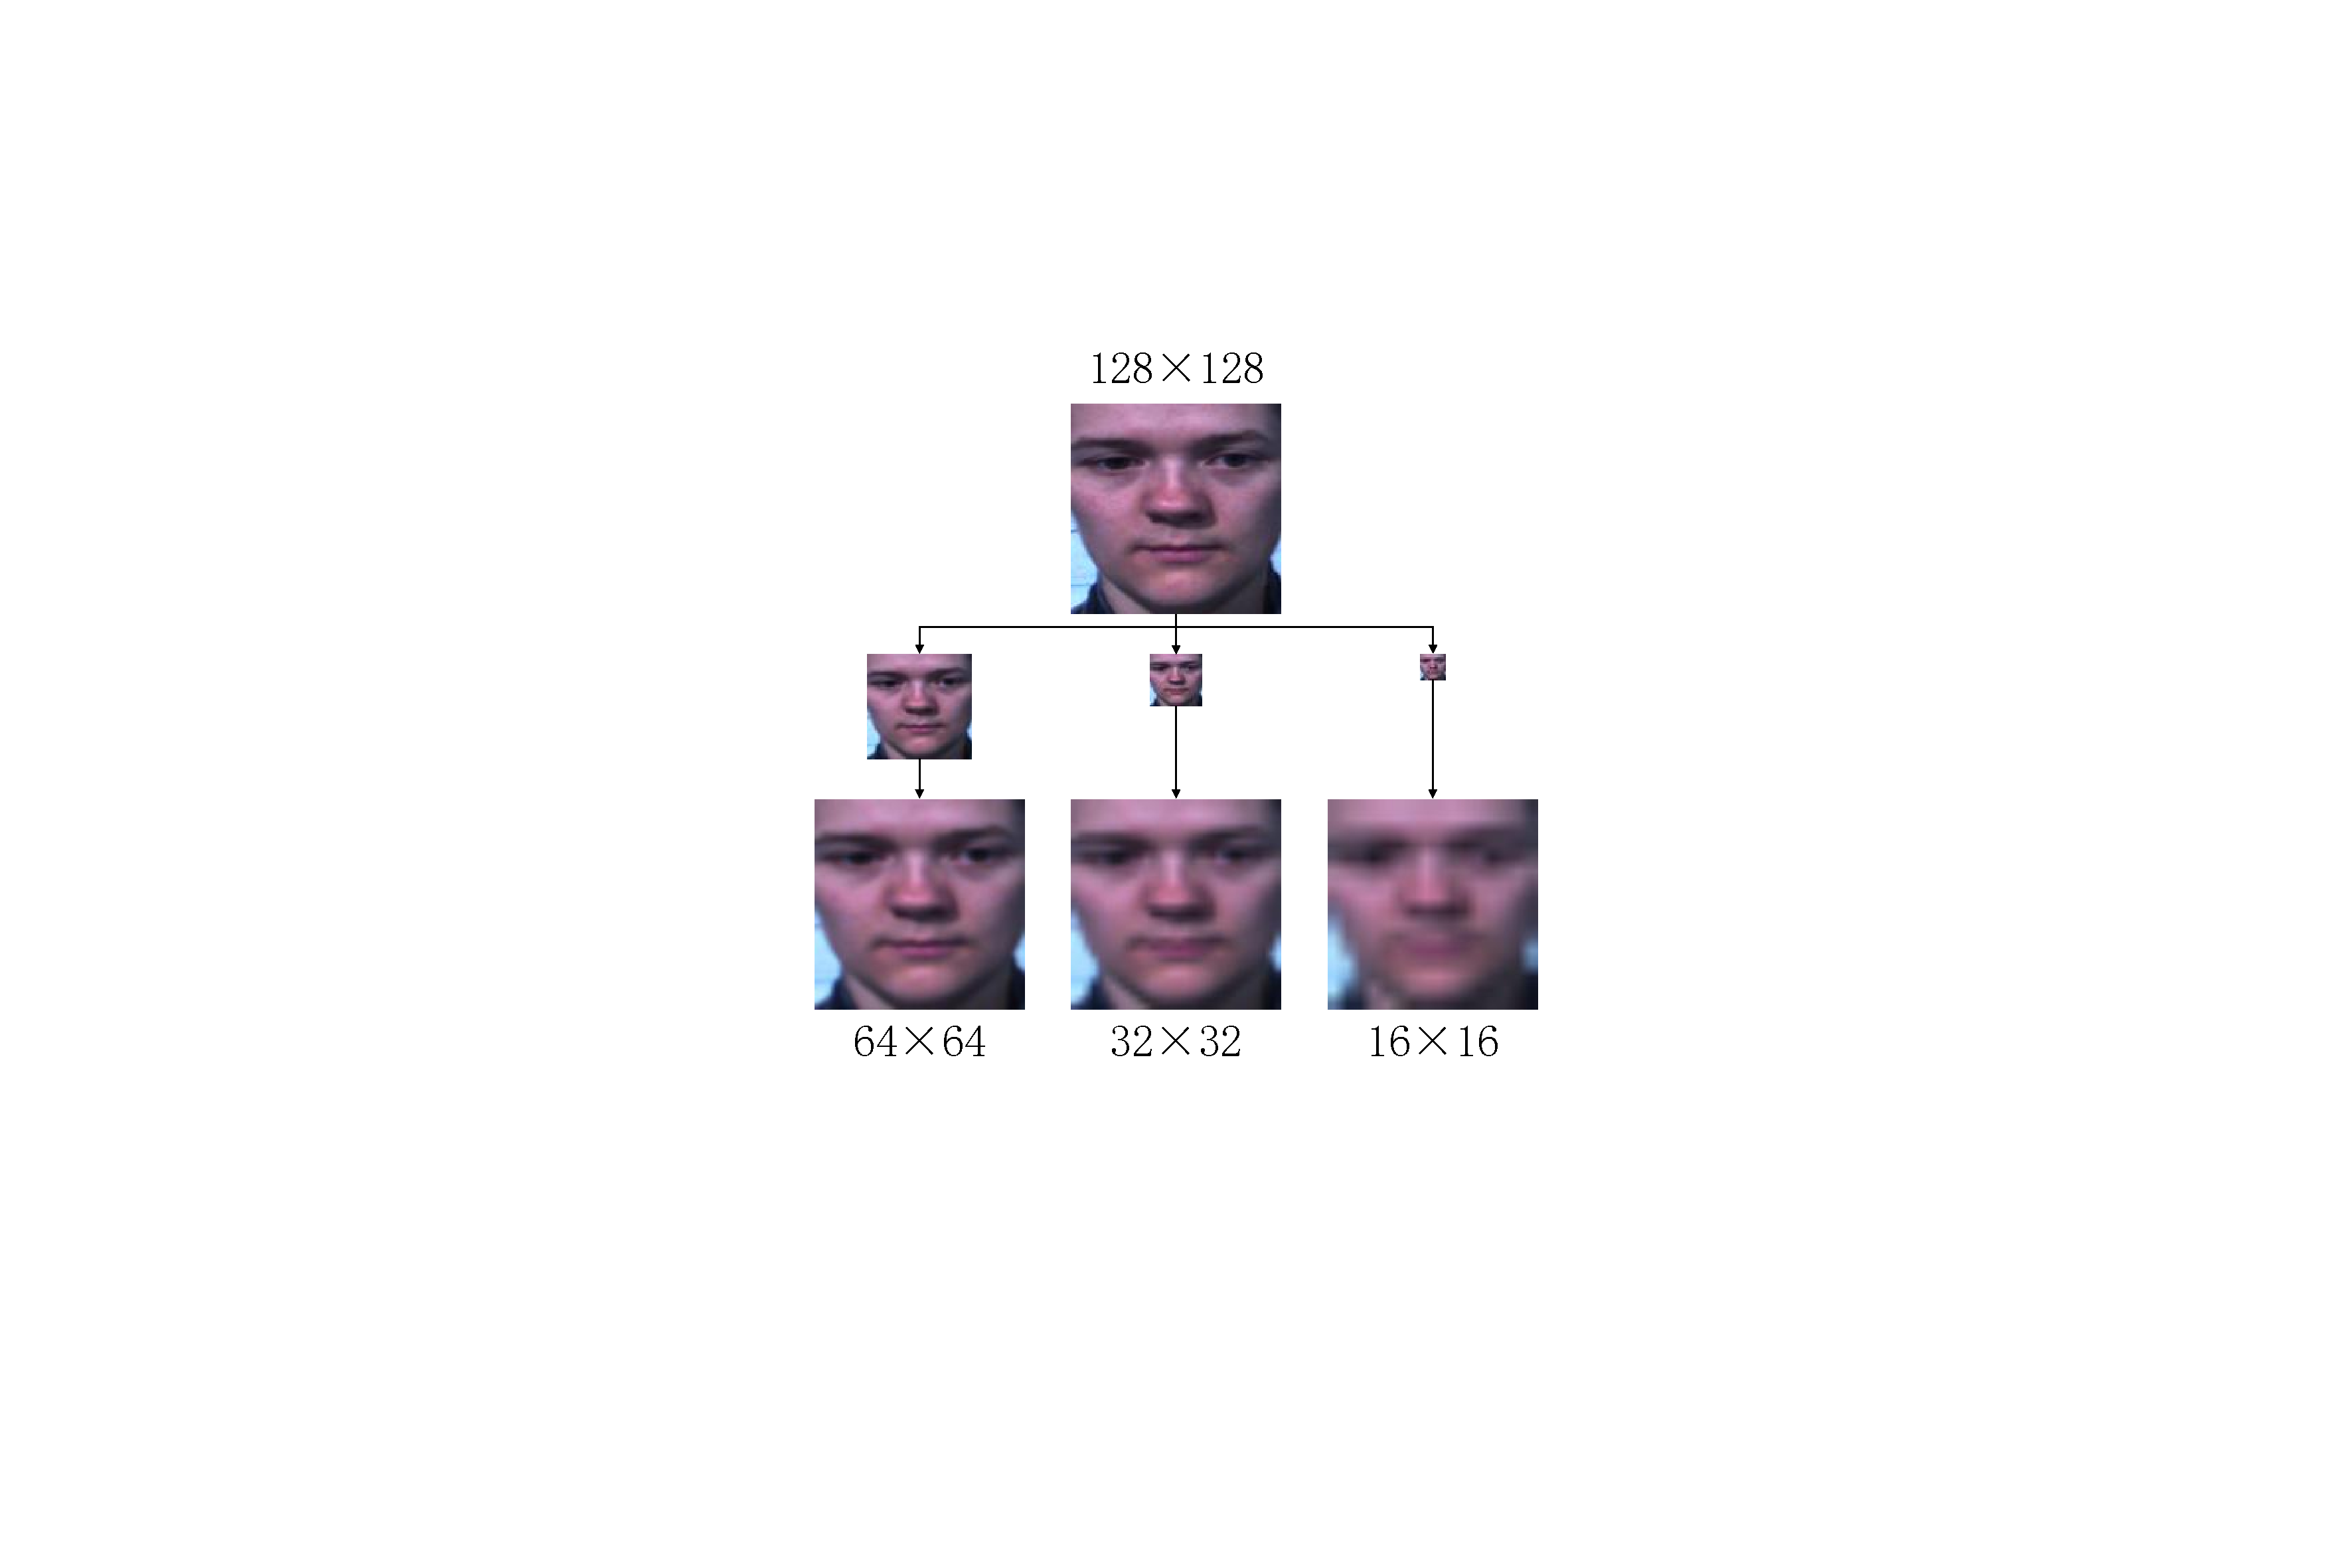
\includegraphics[width=\textwidth]{LR41}
      \caption{}
    \end{subfigure}
    \quad
    \begin{subfigure}[b]{0.35\textwidth}
      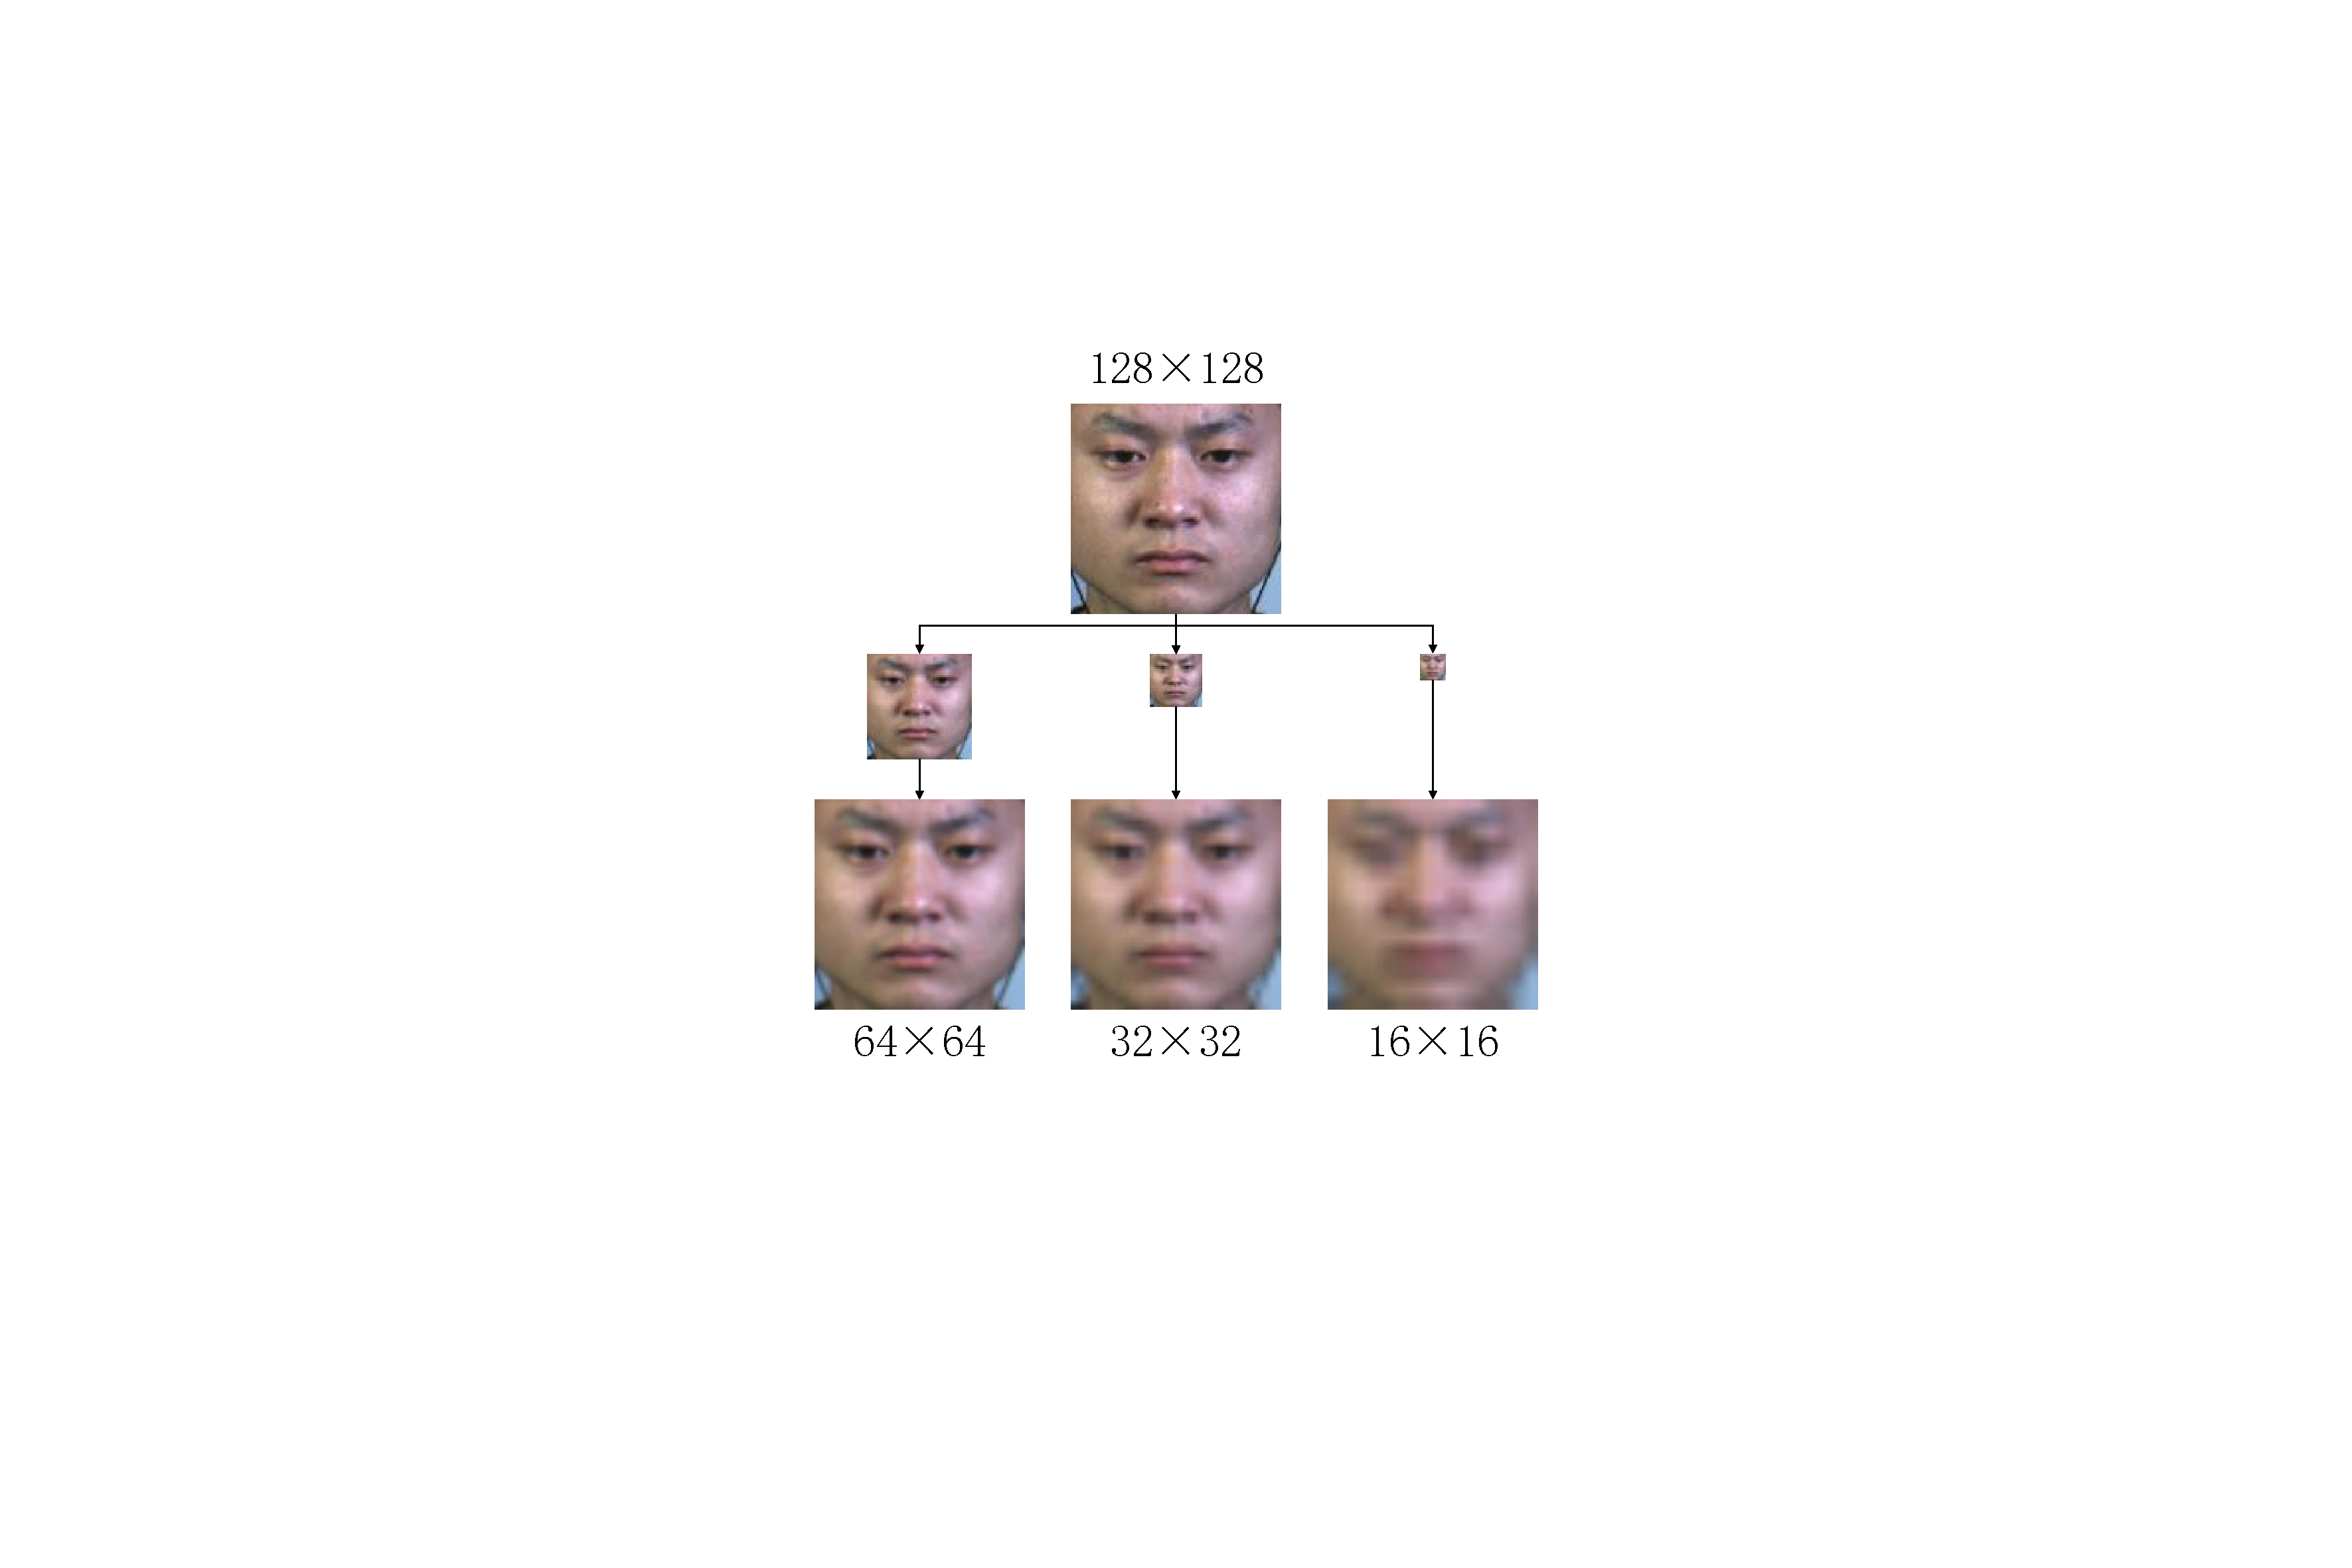
\includegraphics[width=\textwidth]{LR42}
      \caption{}
    \end{subfigure}
    \begin{spacing}{1.0}
    \caption{低分辨率图像}
    \label{fig17}
    \centerline{\footnotesize \textmd{(a) SMIC-HS/SMIC-subHS数据集低分辨率图像,(b) CASME II数据集低分辨率图像}}
    \end{spacing}
\end{figure}

SMIC-HS和SMIC-subHS是SMIC的两个子集。SMIC-HS数据集包含来自16名参与者的164个自发微表情片段,分为三类:积极(51个片段)、消极(70个片段)和惊讶(43个片段)。SMIC-subHS数据集是SMIC-HS的子集,只包含最后8个参与者。前8名受试者的微表达片段数量差异较大,其中3名受试者贡献了整个组近一半的微表达样本,这可能会影响“一受试者退出”的表现,而后8名受试者的(SMIC-subHS)片段数量分布较为均匀。SMIC-subHS数据集中,正负、惊喜片段分别为28、23、20个。同时,CASME II数据集包含26名参与者,分别属于5个不同的类别:惊讶(25个片段)、快乐(32个片段)、其他(99个片段)、厌恶(64个片段)和压抑(27个片段)。表1显示了实验中使用的数据集的摘要。面部高分辨率图像的分辨率设置为$ 128 \times 128 $的实验。$ 128 \times 128 $分辨率的图像下采样乘以2,4,8次获得低分辨率图像(如图6)。这意味着我们评估三个不同层次的低分辨率的面部图像序列(如$ 16 \times 16 $, $ 32 \times 32 $, $ 64 \times 64 $)的微识别任务。

在本节中,利用论文\citepns{shi2018hallucinating}提出的方法将低分辨率图像重建为高分辨率图像,该方法在2.3节中进行了简要介绍。表2-3列出了不同分辨率下重建图像序列的平均峰值信噪比(PSNR)和结构相似度(SSIM)指数。在这里,我们分别使用S64、S32和S16来命名分辨率为$ 64 \times 64 $, $ 32 \times 32 $和$ 16 \times 16 $的重建图像序列。

\begin{table}[!htbp]
  \renewcommand\arraystretch{1.5}
  \centering
  \caption{重建图像序列的平均PSNR(dB)指标}
  \label{tab5}
  \scalebox{0.95}{
  \begin{tabular}{c|ccc}
    \hline
    PSNR (dB) & $ 16 \times 16 $ & $ 32 \times 32 $ & $ 64 \times 64 $ \\ \hline
    SMIC-HS & 31.25 & 37.67 & 44.30 \\
    SMIC-subHS & 31.67 & 38.26 & 43.22 \\
    CASME II & 31.80 & 36.49 & 37.83 \\ \hline
  \end{tabular}}
\end{table}

\begin{table}[!htbp]
  \renewcommand\arraystretch{1.5}
  \centering
  \caption{重建图像序列的平均SSIM指标}
  \label{tab6}
  \scalebox{0.95}{
  \begin{tabular}{c|ccc}
    \hline
    SSIM & $ 16 \times 16 $ & $ 32 \times 32 $ & $ 64 \times 64 $ \\ \hline
    SMIC-HS & 0.9397 & 0.9775 & 0.9883 \\
    SMIC-subHS & 0.8970 & 0.9346 & 0.9424 \\
    CASME II & 0.9439 & 0.9761 & 0.9882 \\ \hline
  \end{tabular}}
\end{table}

如表2和表3所示,重建的人脸图像序列的定量指标(PSNR/SSIM)与输入人脸图像序列的分辨率成正比。例如,在SMIC-HS数据集中,S16的PSNR指数为31.25dB,比S32低6.42dB,比S64低13.05dB。对于SSIM指数,S16达到0.9397,比S32低0.0378,比S64低0.0486。此外,图7给出了重建后的图像序列的视觉表现,也表明了与上述观点相同的结论。

\begin{figure}[!htbp]
  \centering
  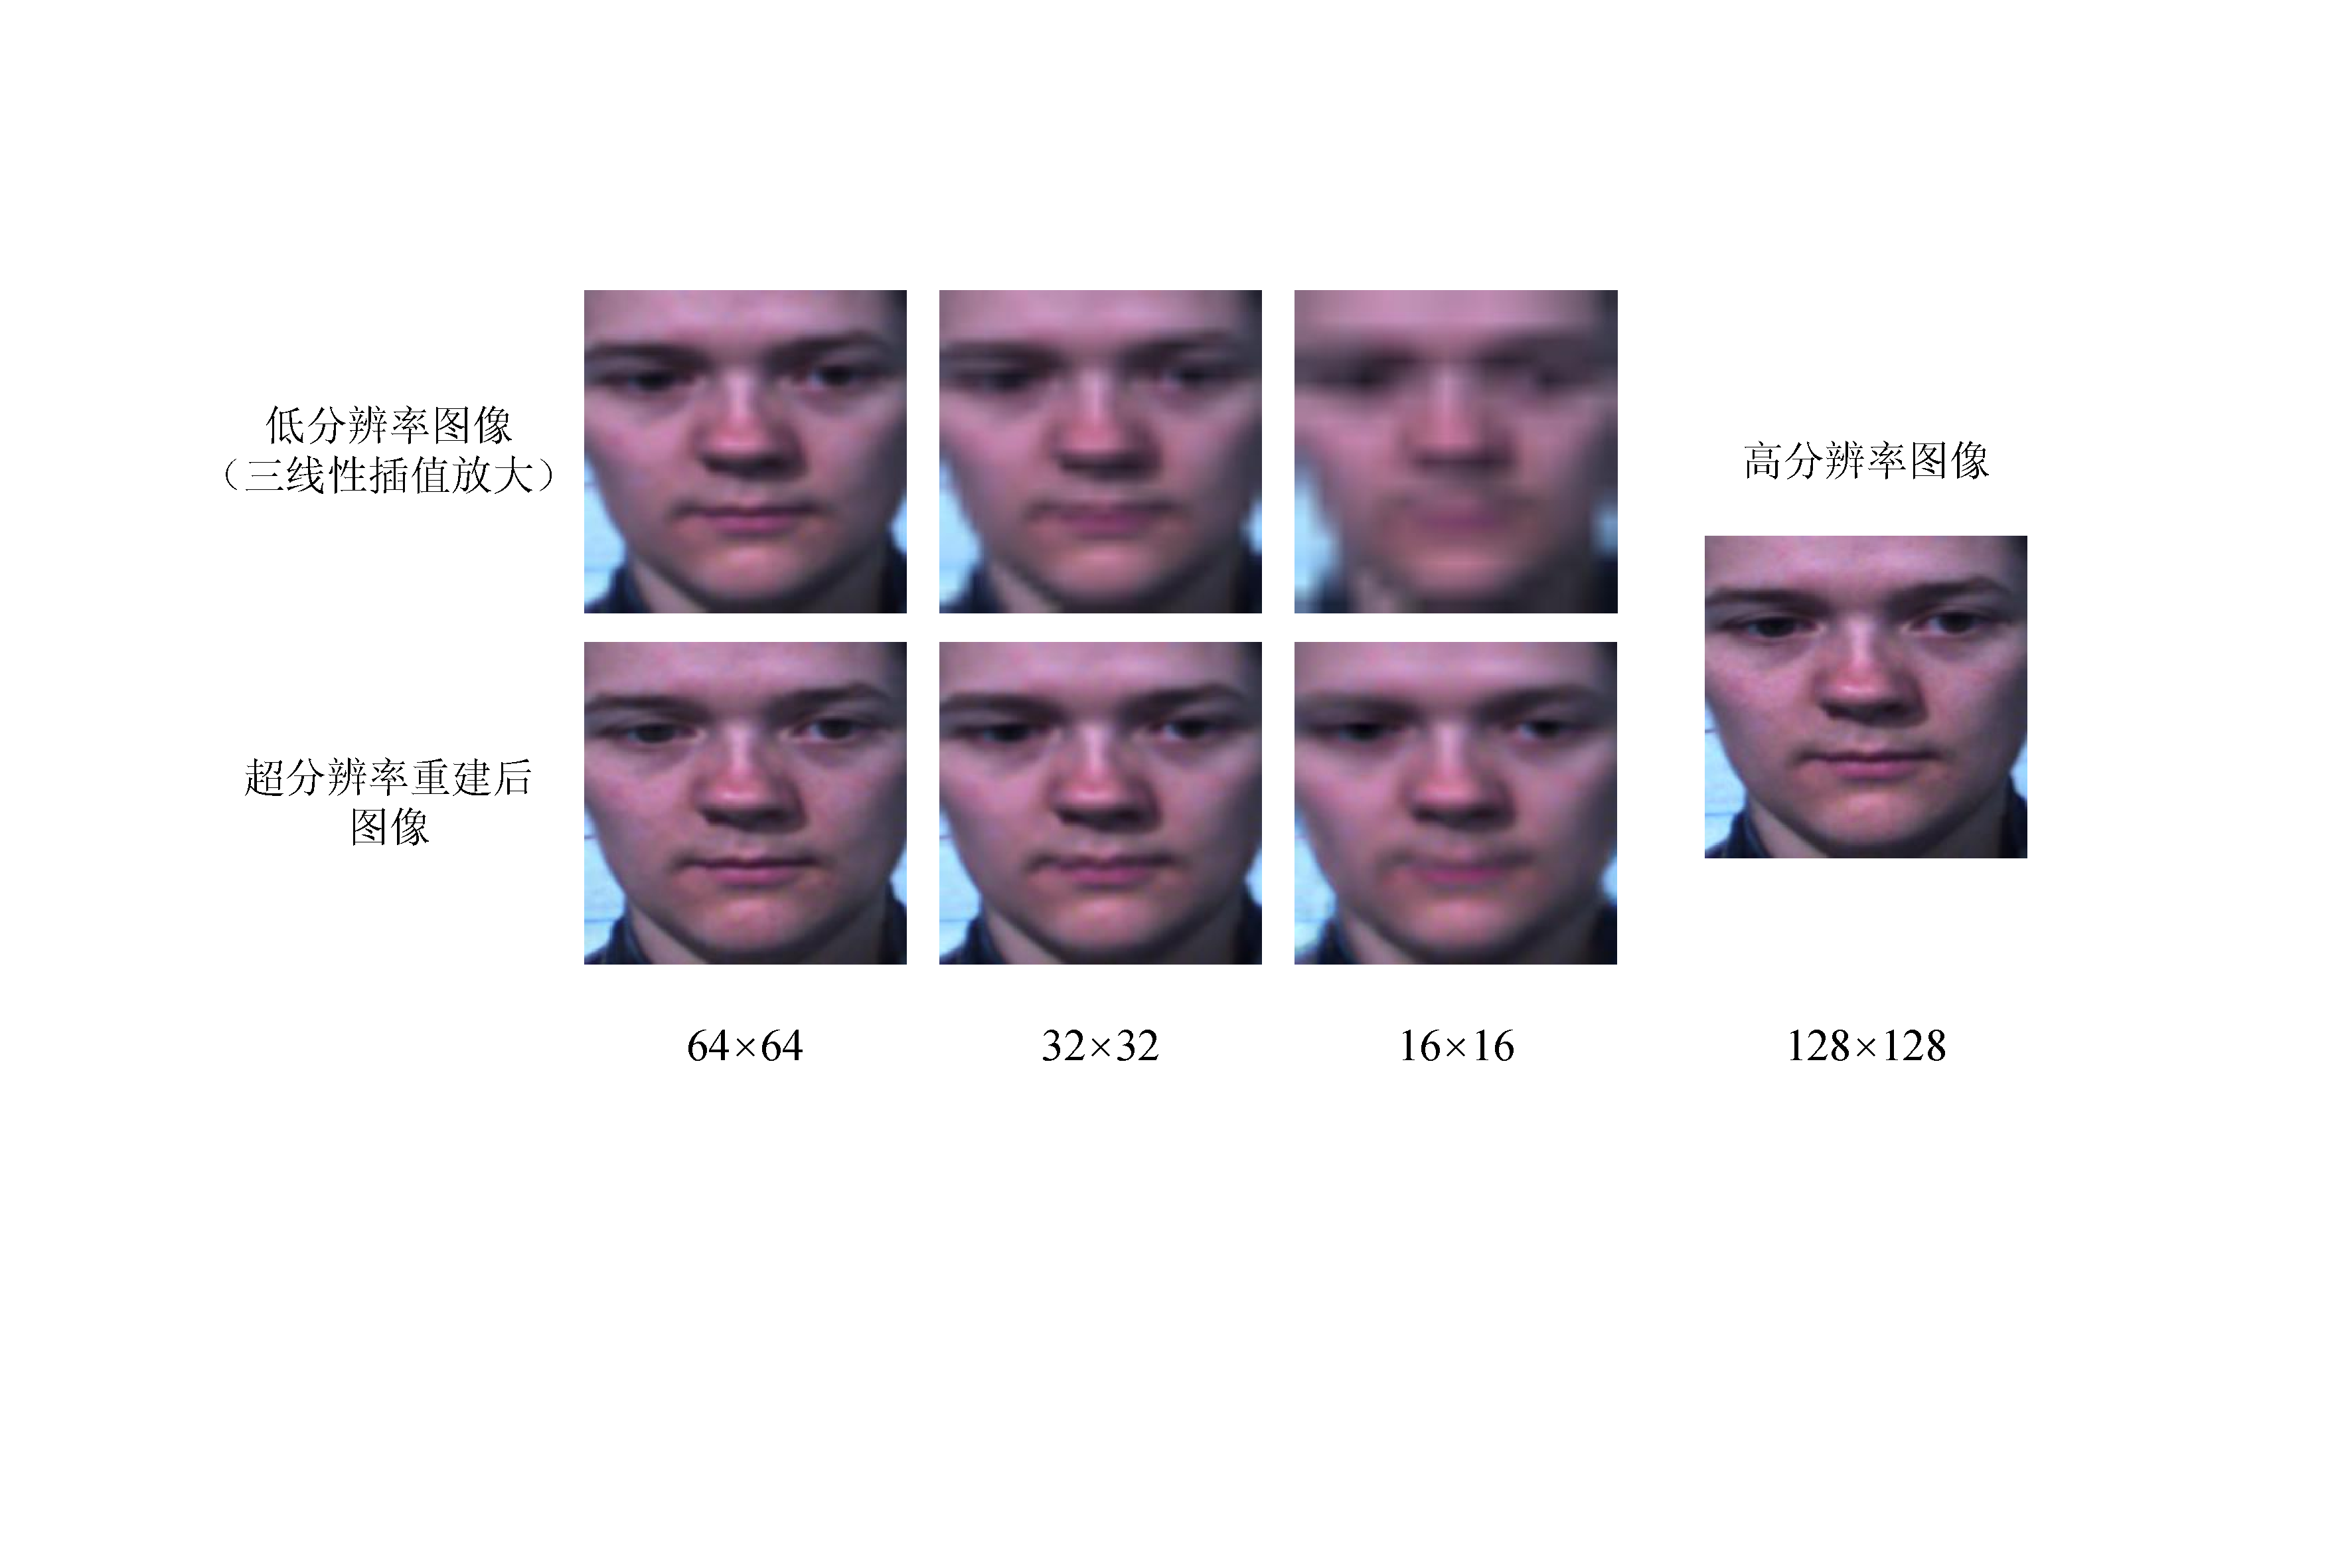
\includegraphics[width=0.75\textwidth]{LR5}
  \caption{不同分辨率图像重建结果比较}
  \label{fig18}
\end{figure}

为了对视频片段的时长进行归一化,使用TIM算法将视频片段的帧数插值为10帧,如2.2节所述。我们应用快速LBP-TOP将视频片段成不同的长方体和提取每个长方体的LBP-TOP特征构成一个完整的功能,使用统一的映射,半径设置为$ r=2 $,和相邻点$p$的数量设置为$ p=8 $。我们使用leave-one-subject-out协议进行实验,即,将一个受试者的所有样本作为测试集,其他受试者的所有样本作为训练集。我们采用LSVM作为分类器,其中惩罚系数$c=1$。

在本节中,我们提出了低分辨率图像序列的微表情识别性能的基线。为了适应不同分辨率的测试样本,我们将训练集从$ 128 \times 128 $下采样到对应的分辨率(即),以便进行分类程序。注意,下采样操作导致微表达式缺乏判别特征。接下来的实验也表明,在非常低的分辨率下,识别的准确率会急剧下降。

图8显示了不同分辨率图像序列在不同数据集上的识别精度。在这里,我们分别使用L64、L32和L16来命名低分辨率图像序列。从图8可以看出,当输入图像序列的分辨率从$ 64 \times 64 $降低到$ 32 \times 32 $时,SMIC-SubHS数据集(蓝色折线)的识别准确率显著降低。同时,我们可以看到低分辨率图像序列(如L16)的准确率相对较低。这一现象表明,低分辨率的图像序列很难获得满意的结果。主要原因是低分辨率导致微表情描述缺乏高频信息和纹理细节。

\begin{figure}[!htbp]
  \centering
  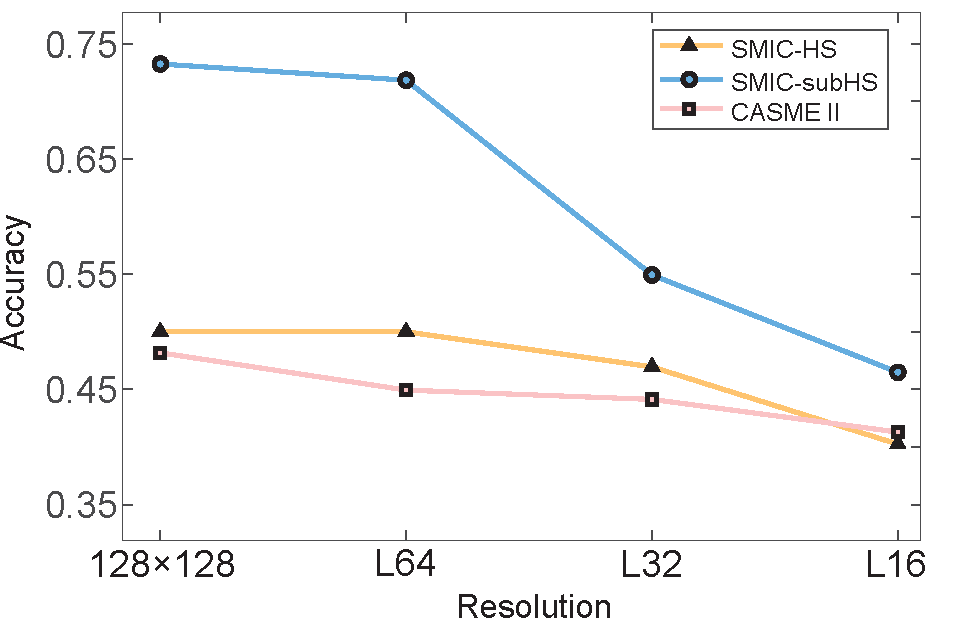
\includegraphics[width=0.60\textwidth]{LR6}
  \caption{不同数据集不同分辨率的图像序列的识别准确度}
  \label{fig19}
\end{figure}

图9为低分辨率图像序列分类结果的混淆矩阵,并以$ 128 \times 128 $分辨率下的性能为参考。我们可以发现,在SMICSubHS数据集(图9第二列)中,当图像序列的分辨率为$ 128 \times 128 $时,混淆矩阵更加集中在对角线上,说明微表情识别方法的识别效果较好。然而,当图像序列的分辨率降低时,混淆矩阵逐渐变差。我们还可以发现,在SMICHS(图9第一列)和CASME II(图9第三列)中,误分类的比例大于SMICsubHS,图8所示的识别准确率也相对较低。对于SMIC-HS来说,上述问题的主要原因可能是后8个受试者(SMIC-subHS数据集)的分布比前8个受试者更加均衡。对于CASME II来说,主要是由于分布不平衡和类别过多。例如,在CASME II数据集中,来自类other的视频片段数量占40.08\%。

\begin{figure}[!htbp]
  \centering
  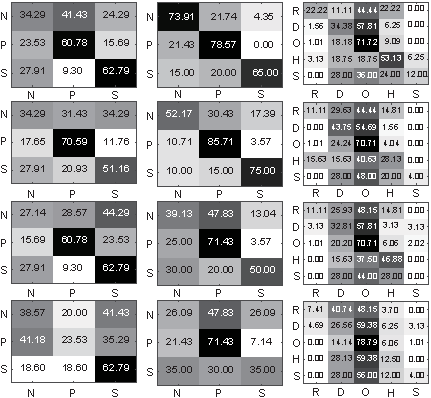
\includegraphics[width=0.75\textwidth]{LR7}
  \caption{不同分辨率图像序列的识别准确度混淆矩阵}
  \label{fig20}
\end{figure}

水平方向,从左往右依次是SMIC-HS数据集、SMIC-subHS数据集和CASME II数据集。垂直方向,从上到下依次是$ 128 \times 128 $分辨率混淆矩阵、$ 64 \times 64 $分辨率混淆矩阵、$ 32 \times 32 $分辨率混淆矩阵和 $ 16 \times 16 $。其中P代表积极(Positive)、N代表消极(Negative)、S代表惊讶(Surprise)、R代表压抑(Repression)、D代表厌恶(Disgust)、O代表其他(Others)、H代表快乐(Happiness)。

在本小节中,我们将在三个数据集上对我们提出的框架进行实验。首先将测试集重构为$ 128 \times 128 $的分辨率,然后在高分辨率空间中进行分类。通过实证分析,选择了最优参数。表4给出了识别精度以及相应的块大小参数设置。从表4可以看出,实验结果有了显著的改善。例如在SMIC-subHS数据集中,$ 64 \times 64 $分辨率下的图像序列识别准确率从71.83\%提高到74.65\%,提高了2.82\%。S32的识别准确率为74.65\%,比L32高19.72\%。S16的识别准确率为73.24\%,比L16高26.76\%。这表明该方法对低分辨率图像序列的微表情识别精度有较好的提高。我们还注意到,与直接将输入作为原始的128128个图像序列相比,该框架使用S64得到了更好的结果。这可能是因为原始SMIC-HS/subHS数据集中的样本在记录过程中存在明显的噪声,使得人脸序列实际上包含了冗余和噪声信息。

超分辨率重建图像序列识别精度的混淆矩阵如图~\ref{fig17}所示。我们展示了$ 128 \times 128 $、S64、S32和S16图像序列根据不同数据集的识别精度。从图~\ref{fig17}可以看出,我们提出的框架的混淆矩阵比图9更集中在对角线上。特别是在$ 16 \times 16 $ SMIC-HS数据集(左下),积极的识别精度有显著提高。此外,我们可以从SMIC-subHS数据集(第二列)的结果中看出,将阴性误分类为阳性的比例显著降低,而将阳性正确分类的比例也得到了大幅提高。不幸的是,尽管CASME II数据集(第三列)的结果有所改善,但每个类别的分类仍然很差,通常错误地划分为其他类别。也许是因为其他微表情包含了所有其他类型的微表情,不包括惊讶、快乐、厌恶和压抑,所以它的分类是混合的。综上所述,从图~\ref{fig17}和图9的对比中我们可以看出,该框架对于低分辨率的微表情识别具有很好的性能提升。

\begin{table}[!htbp]
  \renewcommand\arraystretch{1.5}
  \centering
  \caption{不同分辨率图像在不同数据集上的识别精度比较}
  \label{tab7}
  \scalebox{0.81}{
  \renewcommand{\arraystretch}{1.4}
  \begin{tabular}{c|c|ccc|ccc}
    \hline
    \multirow{2}{*}{Accuracy (\%)} & High-resolution & \multicolumn{3}{c|}{Super-resolution Reconstruction} & \multicolumn{3}{c}{Low-resolution} \\ \cline{2-8}
    & $ 128 \times 128 $ & $ 64 \times 64 $ & $ 32 \times 32 $ & $ 16 \times 16 $ & $ 64 \times 64 $ & $ 32 \times 32 $ & $ 16 \times 16 $ \\ \hline
    SMIC-HS & \begin{tabular}[c]{@{}c@{}}50.00\\ ($ 8 \times 8 \times 2 $)\end{tabular} & \begin{tabular}[c]{@{}c@{}}52.44\\ ($ 5 \times 5\times 2 $)\end{tabular} & \begin{tabular}[c]{@{}c@{}}51.83\\ ($ 5 \times 5 \times 2 $)\end{tabular} & \begin{tabular}[c]{@{}c@{}}51.83\\ ($ 5 \times 5 \times 2 $)\end{tabular} & \begin{tabular}[c]{@{}c@{}}50.00\\ ($ 6 \times 6 \times 5 $)\end{tabular} & \begin{tabular}[c]{@{}c@{}}46.95\\ ($ 6 \times 6 \times 5 $)\end{tabular} & \begin{tabular}[c]{@{}c@{}}40.24\\ ($ 3 \times 3 \times 6 $)\end{tabular} \\
    SMIC-subHS & \begin{tabular}[c]{@{}c@{}}73.24\\ ($ 5 \times 5 \times 2 $)\end{tabular} & \begin{tabular}[c]{@{}c@{}}74.65\\ ($ 5\times 5 \times 2 $)\end{tabular} & \begin{tabular}[c]{@{}c@{}}74.65\\ ($ 5 \times 5 \times 2 $)\end{tabular} & \begin{tabular}[c]{@{}c@{}}73.24\\ ($ 8 \times 8 \times 3 $)\end{tabular} & \begin{tabular}[c]{@{}c@{}}71.83\\ ($ 6 \times 6 \times 2 $)\end{tabular} & \begin{tabular}[c]{@{}c@{}}54.93\\ ($ 6 \times 6 \times 2 $)\end{tabular} & \begin{tabular}[c]{@{}c@{}}46.48\\ ($ 4 \times 4 \times 1 $)\end{tabular} \\
    CASME II & \begin{tabular}[c]{@{}c@{}}48.18\\ ($ 7 \times 7 \times 3 $)\end{tabular} & \begin{tabular}[c]{@{}c@{}}48.18\\ ($ 7 \times 7 \times 5 $)\end{tabular} & \begin{tabular}[c]{@{}c@{}}44.53\\ ($ 7 \times 7 \times 3 $)\end{tabular} & \begin{tabular}[c]{@{}c@{}}42.92\\ ($ 7 \times 7 \times 5 $)\end{tabular} & \begin{tabular}[c]{@{}c@{}}44.94\\ ($ 7 \times 7 \times 1 $)\end{tabular} & \begin{tabular}[c]{@{}c@{}}44.13\\ ($ 4 \times 4 \times 2 $)\end{tabular} & \begin{tabular}[c]{@{}c@{}}41.30\\ ($ 2 \times 2 \times 5 $)\end{tabular} \\ \hline
  \end{tabular} }
\end{table}

High-resolution是指分辨率为$ 128 \times 128 $的图像序列,Super-resolution Reconstruction是指将低分辨率图像序列通过超分辨率重建方法为$ 128 \times 128 $,Low-resolution是指重建前的低分辨率图像序列。$ \mathrm{X} \times \mathrm{Y}  \times \mathrm{T} $指水平、垂直和时间方向块的数量。

\section{本章小结}

本文对低分辨率微表情识别问题进行了全面的研究。我们使用模糊和下采样模型来生成和模拟低分辨率的微表情人脸图像序列。我们在每一帧上使用面部幻觉的方法重建高质量的面部图像序列,增强局部细节,将低质量的图像序列放大到高分辨率的图像序列。然后利用快速LBP-TOP提取动态特征,利用SVM分类器对微表情进行识别。实验结果表明,在低分辨率的微表情识别问题上,该框架在可公开获取的微表情数据集(SMIC-HS、SMIC-subHS、CASME II)上表现良好。

\chapter{基于深度学习方法的低分辨率环境下微表情识别}\label{chap:owner2}

% 为方便使用及更好地展示\LaTeX{}排版的优秀特性,ucasthesis的框架和文件体系进行了细致地处理,尽可能地对各个功能和板块进行了模块化和封装,对于初学者来说,众多的文件目录也许一开始让人觉得有些无所适从,但阅读完下面的使用说明后,会发现原来使用思路是简单而清晰的,而且,当对\LaTeX{}有一定的认识和了解后,会发现其相对Word类排版系统极具吸引力的优秀特性。所以,如果是初学者,请不要退缩,请稍加尝试和坚持,以领略到\LaTeX{}的非凡魅力,并可以通过阅读相关资料如\LaTeX{} Wikibook\citep{wikibook2014latex}来完善自己的使用知识。

\section{数据增强}

% \begin{enumerate}
%     \item 安装软件:根据所用操作系统和章节~\ref{sec:system}中的信息安装\LaTeX{}编译环境。
%     \item 获取模板:下载 \href{https://github.com/mohuangrui/ucasthesis}{ucasthesis} 模板并解压。ucasthesis模板不仅提供了相应的类文件,同时也提供了包括参考文献等在内的完成学位论文的一切要素,所以,下载时,推荐下载整个ucasthesis文件夹,而不是单独的文档类。
%     \item 编译模板:
%         \begin{enumerate}
%             \item Windows:双击运行artratex.bat脚本。
%             \item Linux或MacOS: {\scriptsize \verb|terminal| -> \verb|chmod +x ./artratex.sh| -> \verb|./artratex.sh xa|}
%             \item 任意系统:都可使用\LaTeX{}编辑器打开Thesis.tex文件并选择xelatex编译引擎进行编译。
%         \end{enumerate}
%     \item 错误处理:若编译中遇到了问题,请先查看“常见问题”(章节~\ref{sec:qa})。
% \end{enumerate}
%
% 编译完成即可获得本PDF说明文档。而这也完成了学习使用ucasthesis撰写论文的一半进程。什么?这就学成一半了,这么简单???,是的,就这么简单!

\subsection{数据集混合}

% Thesis.tex为主文档,其设计和规划了论文的整体框架,通过对其的阅读可以了解整个论文框架的搭建。

\subsection{直方图均衡化}

% \begin{itemize}
%     \item Windows:双击Dos脚本artratex.bat可得全编译后的PDF文档,其存在是为了帮助不了解\LaTeX{}编译过程的初学者跨过编译这第一道坎,请勿通过邮件传播和接收此脚本,以防范Dos脚本的潜在风险。
%     \item Linux或MacOS:在terminal中运行
%         \begin{itemize}
%             \item \verb|./artratex.sh xa|:获得全编译后的PDF文档
%             \item \verb|./artratex.sh x|:快速编译模式
%         \end{itemize}
%     \item 全编译指运行 \verb|xelatex+bibtex+xelatex+xelatex| 以正确生成所有的引用链接,如目录,参考文献及引用等。在写作过程中若无添加新的引用,则可用快速编译,即只运行一遍\LaTeX{}编译引擎以减少编译时间。
% \end{itemize}

\subsection{亮度调整}

% 运行编译脚本后,编译所生成的文档皆存于Tmp文件夹内,包括编译得到的PDF文档,其存在是为了保持工作空间的整洁,因为好的心情是很重要的。
\section{P3D ResNet}

在视频分类或理解领域,容易从图像领域的2D卷积联想到用3D卷积来做,虽然用3D卷积进行特征提取可以同时考虑到spatial和temporal维度的特征,但是计算成本和模型存储都太大,因此这篇文章针对视频领域中采用的3D卷积进行改造,提出Pseudo-3D Residual Net (P3D ResNet),思想有点像当年的Inception v3中用1*3和3*1的卷积叠加代替原来的3*3卷积,这篇文章是用1*3*3卷积和3*1*1卷积代替3*3*3卷积(前者用来获取spatial维度的特征,实际上和2D的卷积没什么差别;后者用来获取temporal维度的特征,因为倒数第三维是帧的数量),毕竟这样做可以大大减少计算量,而如果采用3D卷积来做的话,速度和存储正是瓶颈,这也使得像C3D算法的网络深度只有11层,参看Figure1。该文章的网络结构可以直接在3D的ResNet网络上修改得到。顺便提一下,除了采用3D卷积来提取temporal特征外,还可以采用LSTM来提取,这也是当前视频研究的一个方向。

Figure1是几个模型在层数、模型大小和在Sports-1M数据集上的视频分类效果对比,其中的P3D ResNet是在ResNet 152基础上修改得到的,深度之所以不是152,是因为改造后的每个residual结构不是原来ResNet系列的3个卷积层,而是3或4个卷积层,详细可以看Figure3,所以最后网络深度是199层。官方github代码中的网络就是199层的。ResNet 152是直接在Sports-1M数据集上fine tune得到的。可以看出199层的P3D ResNet虽然在模型大小上比ResNet-152(此处ResNet-152是在sports-1M数据集上fine tune得到的)大一些,但是准确率提升比较明显,与C3D(此处C3D是直接在sports-1M数据集上从头开始训练得到的)的对比在效果和模型大小上都有较大改进,除此之外,速度的提升也是亮点,后面有详细的速度对比。

\begin{figure}[]
\centering
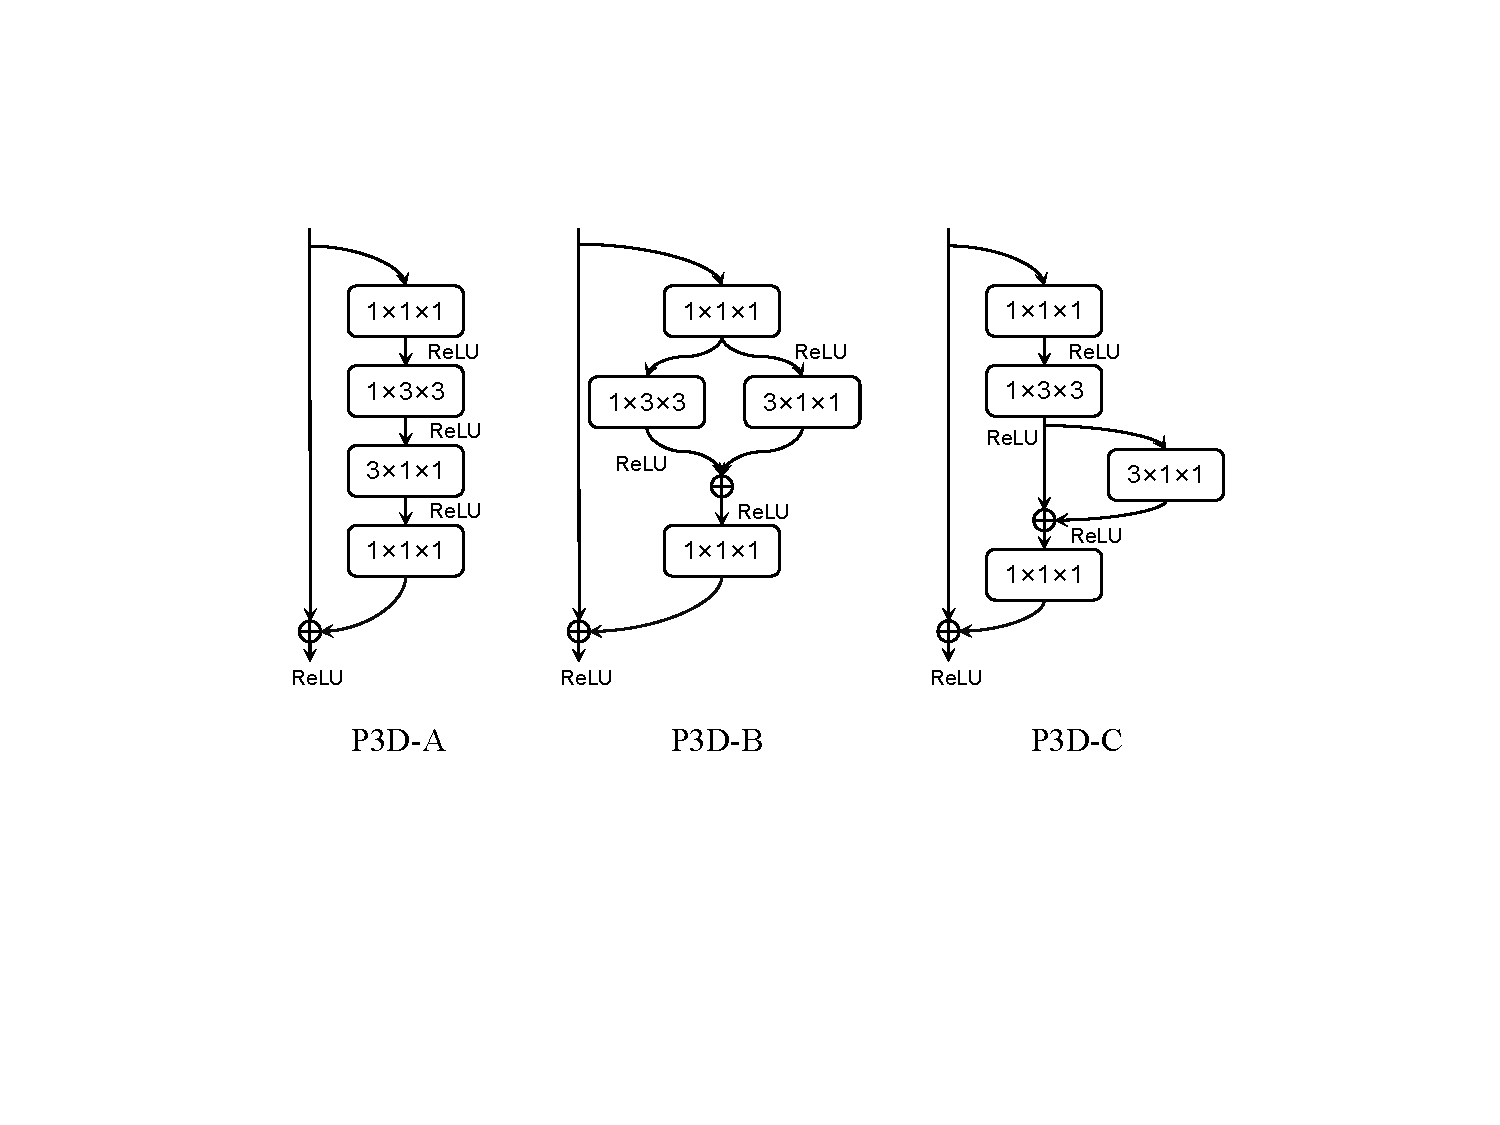
\includegraphics[width=0.75\textwidth]{P3D0}
\caption{伪3D残差网络三种设计模型}
\label{fig18}
\end{figure}

\subsection{1}

% 包含ucasthesis文档类的定义文件和配置文件,通过对它们的修改可以实现特定的模版设定。若需更新模板,一般只需用新的样式文件替换旧的即可。
%
% \begin{enumerate}
%     \item ucasthesis.cls:文档类定义文件,论文的最核心的格式即通过它来定义的。
%     \item ucasthesis.cfg:文档类配置文件,设定如目录显示为“目~录”而非“目录”。
%     \item artratex.sty: 常用宏包及文档设定,如参考文献样式、文献引用样式、页眉页脚设定等。这些功能具有开关选项,常只需在Thesis.tex中的如下命令中进行启用即可,一般无需修改artratex.sty本身。
%
%         \path{\usepackage[options]{artratex}}
%     \item artracom.sty:自定义命令以及添加宏包的推荐放置位置。
% \end{enumerate}

\subsection{2}

% 文件夹内为论文的所有实体内容,正常情况下,这也是\textbf{使用ucasthesis撰写学文论文时,主要关注和修改的一个位置,注:所有文件都必须采用UTF-8编码,否则编译后将出现乱码文本},详细分类介绍如下:
%
% \begin{itemize}
%     \item Frontpage.tex:为论文中英文封面及中英文摘要。\textbf{论文封面会根据英文学位名称如Bachelor,Master,或是Doctor自动切换为相应的格式}。
%     \item Mainmatter.tex:索引需要出现的Chapter。开始写论文时,可以只索引当前章节,以快速编译查看,当论文完成后,再对所有章节进行索引即可。
%     \item Chap{\_}xxx.tex:为论文主体的各个章节,可根据需要添加和撰写。
%     \item Appendix.tex:为附录内容
%     \item Backmatter.tex:为发表文章信息和致谢部分等。
% \end{itemize}

\subsection{3}

% 用于放置论文中所需要的图类文件,支持格式有:.jpg, .png, .pdf。其中,\verb|ucas_logo.pdf|为国科大校徽。不建议为各章节图片建子目录,即使图片众多,若命名规则合理,图片查询亦是十分方便。

\section{实验设置及分析}

\subsection{1}

% \begin{enumerate}
%     \item ref.bib:参考文献信息库。
%     \item gbt7714-xxx.bst:符合国标的文献样式定义文件。由 \href{https://github.com/zepinglee/gbt7714-bibtex-style}{zepinglee}  开发,并满足最新国标要求。与文献样式有关的问题,请查阅开发者所提供的文档,并建议适当追踪其更新。
% \end{enumerate}
\subsection{2}

\subsection{3}

\section{总结}

\chapter{系统设计}\label{chap:system}

% 为方便使用及更好地展示\LaTeX{}排版的优秀特性,ucasthesis的框架和文件体系进行了细致地处理,尽可能地对各个功能和板块进行了模块化和封装,对于初学者来说,众多的文件目录也许一开始让人觉得有些无所适从,但阅读完下面的使用说明后,会发现原来使用思路是简单而清晰的,而且,当对\LaTeX{}有一定的认识和了解后,会发现其相对Word类排版系统极具吸引力的优秀特性。所以,如果是初学者,请不要退缩,请稍加尝试和坚持,以领略到\LaTeX{}的非凡魅力,并可以通过阅读相关资料如\LaTeX{} Wikibook\citep{wikibook2014latex}来完善自己的使用知识。

\section{需求分析}

% \begin{enumerate}
%     \item 安装软件:根据所用操作系统和章节~\ref{sec:system}中的信息安装\LaTeX{}编译环境。
%     \item 获取模板:下载 \href{https://github.com/mohuangrui/ucasthesis}{ucasthesis} 模板并解压。ucasthesis模板不仅提供了相应的类文件,同时也提供了包括参考文献等在内的完成学位论文的一切要素,所以,下载时,推荐下载整个ucasthesis文件夹,而不是单独的文档类。
%     \item 编译模板:
%         \begin{enumerate}
%             \item Windows:双击运行artratex.bat脚本。
%             \item Linux或MacOS: {\scriptsize \verb|terminal| -> \verb|chmod +x ./artratex.sh| -> \verb|./artratex.sh xa|}
%             \item 任意系统:都可使用\LaTeX{}编辑器打开Thesis.tex文件并选择xelatex编译引擎进行编译。
%         \end{enumerate}
%     \item 错误处理:若编译中遇到了问题,请先查看“常见问题”(章节~\ref{sec:qa})。
% \end{enumerate}
%
% 编译完成即可获得本PDF说明文档。而这也完成了学习使用ucasthesis撰写论文的一半进程。什么?这就学成一半了,这么简单???,是的,就这么简单!

\section{功能设计}

\subsection{功能图}

% Thesis.tex为主文档,其设计和规划了论文的整体框架,通过对其的阅读可以了解整个论文框架的搭建。

\subsection{时序图}

% \begin{itemize}
%     \item Windows:双击Dos脚本artratex.bat可得全编译后的PDF文档,其存在是为了帮助不了解\LaTeX{}编译过程的初学者跨过编译这第一道坎,请勿通过邮件传播和接收此脚本,以防范Dos脚本的潜在风险。
%     \item Linux或MacOS:在terminal中运行
%         \begin{itemize}
%             \item \verb|./artratex.sh xa|:获得全编译后的PDF文档
%             \item \verb|./artratex.sh x|:快速编译模式
%         \end{itemize}
%     \item 全编译指运行 \verb|xelatex+bibtex+xelatex+xelatex| 以正确生成所有的引用链接,如目录,参考文献及引用等。在写作过程中若无添加新的引用,则可用快速编译,即只运行一遍\LaTeX{}编译引擎以减少编译时间。
% \end{itemize}

\subsection{等}

% 运行编译脚本后,编译所生成的文档皆存于Tmp文件夹内,包括编译得到的PDF文档,其存在是为了保持工作空间的整洁,因为好的心情是很重要的。

\section{界面设计}

\section{小节}

\chapter{总结与展望}\label{chap:conclusions}

The current ME studies can be continued and improved from four aspects in future work. First, about the ME database: more spontaneous ME data are still needed in order to develop more sophisticate computational models. Compared to ordinary FE databases, the size of current ME databases are not big enough. Future collection of ME data can be improved from three ways: the first is to increase the sample size; the second is to involve AU labelling; the third is to include depth information to build 3D ME models. A large 3D ME database is now under construction with collaboration of a group of UK researchers.
在今后的工作中,可以从四个方面继续和完善目前ME的研究。首先,关于ME数据库:为了开发更复杂的计算模型,仍然需要更多自发的ME数据。与普通FE数据库相比,目前ME数据库的规模还不够大。未来ME数据的收集可以通过三种方式进行改进:一是增加样本量;二是涉及AU标签;第三个是包含深度信息来构建3D ME模型。一组英国研究人员正在合作建立一个大型3D ME数据库。

Second, about ME spotting: the framework using feature difference analysis for ME spotting described in Section 2.5 was the first method proposed for spotting MEs from spontaneous long videos. One challenge of the current spotting framework is that there are other brief but non-emotional movements (e.g., eye blinks) that need to be ruled out from MEs. In future, more refined spotting method will be developed on the AU level, so that non-emotional brief movements can be ruled out to reduce the false positive rate. Besides, future ME spotting method will also try to target at providing more precise temporal information of the ME including the onset, apex and offset frames.
第二,关于ME点测:2.5节中描述的ME点测特征差异分析框架是第一个从自发长视频中提取MEs的方法。当前的识别框架的一个挑战是,需要排除MEs中其他短暂但非情绪的动作(例如眨眼)。未来将在AU水平上开发更精细的点样方法,排除非情绪短暂运动,降低假阳性率。此外,未来的ME定位方法也将致力于提供更精确的ME的时间信息,包括起始帧、顶点帧和偏移帧。

Third, about ME recognition: the latest method proposed in paper III showed advantage over previous methods by employing one extra step to magnify the subtle motions. Other video processing methods will be explored and added to the framework, if they are demonstrated to be helpful for the ME recognition task. More sophisticate machine learning models will be studied including deep learning models. It is also planned to use 3D information for ME recognition when the new 3D ME database is finished.
第三,关于ME识别:第三篇论文中提出的最新方法比之前的方法有优势,多了一步放大了细微的运动。如果其他视频处理方法被证明对ME识别任务有帮助,我们将探索并添加到该框架中。将研究更复杂的机器学习模型,包括深度学习模型。也计划在新的3D ME数据库完成后使用3D信息进行ME识别。

Fourth, about integrated ME spotting and recognition systems: after progresses are made for both ME recognition methods and ME spotting methods, it is also planned to build advanced integrated systems for more accurate ME spotting and recognition.
第四,ME点测与识别集成系统:在ME点测与识别方法取得进展后,计划构建先进的ME点测与识别集成系统,提高ME点测与识别的准确率。

\section{总结}


\section{存在的问题与展望}

\subsection{存在的问题}

\subsection{展望}

%---------------------------------------------------------------------------%
% main content
%-
%-> Appendix
%-
\cleardoublepage%
\appendix% initialize the environment
\chapter{附录}

学位论文是研究生科研工作成果的集中体现,是评判学位申请者学术水平、授予其学位的主要依据,是科研领域重要的文献资料。根据《科学技术报告、学位论文和学术论文的编写格式》(GB/T 7713-1987)、《学位论文编写规则》(GB/T 7713.1-2006)和《文后参考文献著录规则》(GB7714—87)等国家有关标准,结合中国科学院大学(以下简称“国科大”)的实际情况,特制订本规定。

\section{论文无附录者无需附录部分}

\section{测试公式编号} \label{sec:testmath}

\begin{equation} \label{eq:appedns}
    \begin{cases}
        \frac{\partial \rho}{\partial t} + \nabla\cdot(\rho\Vector{V}) = 0 \ \mathrm{times\ font\ test}\\
        \frac{\partial (\rho\Vector{V})}{\partial t} + \nabla\cdot(\rho\Vector{V}\Vector{V}) = \nabla\cdot\Tensor{\sigma} \ \text{times font test}\\
        \frac{\partial (\rho E)}{\partial t} + \nabla\cdot(\rho E\Vector{V}) = \nabla\cdot(k\nabla T) + \nabla\cdot(\Tensor{\sigma}\cdot\Vector{V})
    \end{cases}
\end{equation}
\begin{equation}
    \frac{\partial }{\partial t}\int\limits_{\Omega} u \, \mathrm{d}\Omega + \int\limits_{S} \unitVector{n}\cdot(u\Vector{V}) \, \mathrm{d}S = \dot{\phi}
\end{equation}

\section{测试生僻字}

霜蟾盥薇曜灵霜颸妙鬘虚霩淩澌菀枯菡萏泬寥窅冥毰毸濩落霅霅便嬛岧峣瀺灂姽婳愔嫕飒纚棽俪緸冤莩甲摛藻卮言倥侗椒觞期颐夜阑彬蔚倥偬澄廓簪缨陟遐迤逦缥缃鹣鲽憯懔闺闼璀错媕婀噌吰澒洞阛闠覼缕玓瓑逡巡諓諓琭琭瀌瀌踽踽叆叇氤氲瓠犀流眄蹀躞赟嬛茕頔璎珞螓首蘅皋惏悷缱绻昶皴皱颟顸愀然菡萏卑陬纯懿犇麤掱暒 墌墍墎墏墐墒墒墓墔墕墖墘墖墚墛坠墝增墠墡墢墣墤墥墦墧墨墩墪樽墬墭堕墯墰墱墲坟墴墵垯墷墸墹墺墙墼墽垦墿壀壁壂壃壄壅壆坛壈壉壊垱壌壍埙壏壐壑壒压壔壕壖壗垒圹垆壛壜壝垄壠壡坜壣壤壥壦壧壨坝塆圭嫶嫷嫸嫹嫺娴嫼嫽嫾婳妫嬁嬂嬃嬄嬅嬆嬇娆嬉嬊娇嬍嬎嬏嬐嬑嬒嬓嬔嬕嬖嬗嬘嫱嬚嬛嬜嬞嬟嬠嫒嬢嬣嬥嬦嬧嬨嬩嫔嬫嬬奶嬬嬮嬯婴嬱嬲嬳嬴嬵嬶嬷婶嬹嬺嬻嬼嬽嬾嬿孀孁孂娘孄孅孆孇孆孈孉孊娈孋孊孍孎孏嫫婿媚嵭嵮嵯嵰嵱嵲嵳嵴嵵嵶嵷嵸嵹嵺嵻嵼嵽嵾嵿嶀嵝嶂嶃崭嶅嶆岖嶈嶉嶊嶋嶌嶍嶎嶏嶐嶑嶒嶓嵚嶕嶖嶘嶙嶚嶛嶜嶝嶞嶟峤嶡峣嶣嶤嶥嶦峄峃嶩嶪嶫嶬嶭崄嶯嶰嶱嶲嶳岙嶵嶶嶷嵘嶹岭嶻屿岳帋巀巁巂巃巄巅巆巇巈巉巊岿巌巍巎巏巐巑峦巓巅巕岩巗巘巙巚帠帡帢帣帤帨帩帪帬帯帰帱帲帴帵帷帹帺帻帼帽帾帿幁幂帏幄幅幆幇幈幉幊幋幌幍幎幏幐幑幒幓幖幙幚幛幜幝幞帜幠幡幢幤幥幦幧幨幩幪幭幮幯幰幱庍庎庑庖庘庛庝庠庡庢庣庤庥庨庩庪庬庮庯庰庱庲庳庴庵庹庺庻庼庽庿廀厕廃厩廅廆廇廋廌廍庼廏廐廑廒廔廕廖廗廘廙廛廜廞庑廤廥廦廧廨廭廮廯廰痈廲廵廸廹廻廼廽廿弁弅弆弇弉弖弙弚弜弝弞弡弢弣弤弨弩弪弫弬弭弮弰弲弪弴弶弸弻弼弽弿彖彗彘彚彛彜彝彞彟彴彵彶彷彸役彺彻彽彾佛徂徃徆徇徉后徍徎徏径徒従徔徕徖徙徚徛徜徝从徟徕御徢徣徤徥徦徧徨复循徫旁徭微徯徰徱徲徳徴徵徶德徸彻徺忁忂惔愔忇忈忉忔忕忖忚忛応忝忞忟忪挣挦挧挨挩挪挫挬挭挮挰掇授掉掊掋掍掎掐掑排掓掔掕挜掚挂掜掝掞掟掠采探掣掤掦措掫掬掭掮掯掰掱掲掳掴掵掶掸掹掺掻掼掽掾掿拣揁揂揃揅揄揆揇揈揉揊揋揌揍揎揑揓揔揕揖揗揘揙揤揥揦揧揨揫捂揰揱揲揳援揵揶揷揸揻揼揾揿搀搁搂搃搄搅搇搈搉搊搋搌搎搏搐搑搒摓摔摕摖摗摙摚摛掼摝摞摠摡斫斩斮斱斲斳斴斵斶斸旪旫旮旯晒晓晔晕晖晗晘晙晛晜晞晟晠晡晰晣晤晥晦晧晪晫晬晭晰晱晲晳晴晵晷晸晹晻晼晽晾晿暀暁暂暃暄暅暆暇晕晖暊暋暌暍暎暏暐暑暒暓暔暕暖暗旸暙暚暛暜暝暞暟暠暡暣暤暥暦暧暨暩暪暬暭暮暯暰昵暲暳暴暵暶暷暸暹暺暻暼暽暾暿曀曁曂曃晔曅曈曊曋曌曍曎曏曐曑曒曓曔曕曗曘曙曚曛曜曝曞曟旷曡曢曣曤曥曦曧昽曩曪曫晒曭曮曯椗椘椙椚椛検椝椞椟椠椡椢椣椤椥椦椧椨椩椪椫椬椭椮椯椰椱椲椳椴椵椶椷椸椹椺椻椼椽椾椿楀楁楂楃楅楆楇楈楉杨楋楌楍榴榵榶榷榸榹榺榻榼榽榾桤槀槁槂盘槄槅槆槇槈槉槊构槌枪槎槏槐槑槒杠槔槕槖槗滙滛滜滝滞滟滠滢滣滦滧滪滫沪滭滮滰滱渗滳滵滶滹滺浐滼滽漀漃漄漅漈漉溇漋漌漍漎漐漑澙熹漗漘漙沤漛漜漝漞漟漡漤漥漦漧漨漪渍漭漮漯漰漱漳漴溆漶漷漹漺漻漼漽漾浆潀颍潂潃潄潅潆潇潈潉潊潋潌潍潎潏潐潒潓洁潕潖潗潘沩潚潜潝潞潟潠潡潢潣润潥潦潧潨潩潪潫潬潭浔溃潱潲潳潴潵潶滗潸潹潺潻潼潽潾涠澁澄澃澅浇涝澈澉澊澋澌澍澎澏湃澐澑澒澓澔澕澖涧澘澙澚澛澜澝澞澟渑澢澣泽浍澯澰淀澲澳澴澵澶澷澸潇潆瀡瀢瀣瀤瀥潴泷濑瀩瀪瀫瀬瀭瀮瀯弥瀱潋瀳瀴瀵瀶瀷瀸瀹瀺瀻瀼瀽澜瀿灀灁瀺灂沣滠灅灆灇灈灉灊灋灌灍灎灏灐洒灒灓漓灖灗滩灙灚灛灜灏灞灟灠灡灢湾滦灥灦灧灨灪燝燞燠燡燢燣燤燥灿燧燨燩燪燫燮燯燰燱燲燳烩燵燵燸燹燺薰燽焘燿爀爁爂爃爄爅爇爈爉爊爋爌烁爎爏爑爒爓爔爕爖爗爘爙爚烂爜爝爞爟爠爡爢爣爤爥爦爧爨爩猽猾獀犸獂獆獇獈獉獊獋獌獍獏獐獑獒獓獔獕獖獗獘獙獚獛獜獝獞獟獠獡獢獣獤獥獦獧獩狯猃獬獭狝獯狞獱獳獴獶獹獽獾獿猡玁玂玃。
% appendix content
%-
%-> Backmatter: bibliography, glossary, index
%-
\backmatter% initialize the environment
\intotoc{\bibname}% add link to contents table and bookmark
\bibliography{Biblio/ref}% bibliography
\chapter{攻读博士/硕士学位期间取得的科研成果}


\section*{1.发表学术论文}

[1] ucasthesis: A LaTeX Thesis Template for the University of Chinese Academy of Sciences, 2014.


\section*{2.申请(授权)专利}

(无专利时此项不必列出)

\section*{3.参与科研项目及科研获奖 }

可以随意添加新的条目或是结构。

% \thispagestyle{noheaderstyle}% 如果需要移除当前页的页眉
%\pagestyle{noheaderstyle}% 如果需要移除整章的页眉

\cleardoublepage[plain]% 让文档总是结束于偶数页,可根据需要设定页眉页脚样式,如 [noheaderstyle]
% other information
\chapter{作者简介}

\section*{1.基本情况}

吴凌云,福建省屏南县人,中国科学院数学与系统科学研究院博士研究生。

\section*{2.教育背景}

2008.08~2012.07西北大学,本科,专业:

2012.09~       西北大学,硕士研究生,专业:

\section*{3.攻读硕士学位期间的其它奖励}

可以随意添加新的条目或是结构。

% \thispagestyle{noheaderstyle}% 如果需要移除当前页的页眉
%\pagestyle{noheaderstyle}% 如果需要移除整章的页眉

\cleardoublepage[plain]% 让文档总是结束于偶数页,可根据需要设定页眉页脚样式,如 [noheaderstyle]
% other information
\end{document}
%---------------------------------------------------------------------------%
